\documentclass{article}
\usepackage{tikz}
\usepackage{siunitx}
\usepackage{float}

\usetikzlibrary{arrows,shapes}
\usepackage{xifthen}

%\usetikzlibrary{external}
%\tikzexternalize[prefix=figures/]

\begin{document}

\section{Basic plots}
\label{sec:basic}

\begin{figure}[H]
  \centering
  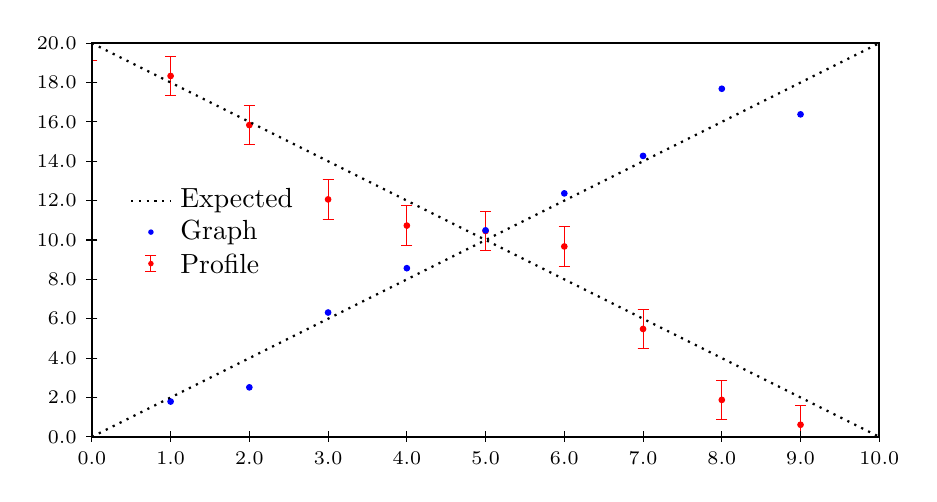
\begin{tikzpicture}
\begin{scope}[]
\clip (0,0) rectangle (10,5);
\draw[draw=red,fill=red] (0.0,4.78456024959082) -- (0.0,5.28456024959082);
\node at (0.0,5.03456024959082) [draw=red,fill=red,circle,inner sep=0pt,minimum width =2pt,minimum height=2pt] {}; 
\draw[draw=red,fill=red] (0.0cm -2pt,4.78456024959082) -- (0.0cm + 2pt,4.78456024959082);
\draw[draw=red,fill=red] (0.0cm -2pt,5.28456024959082) -- (0.0cm + 2pt,5.28456024959082);
\draw[draw=red,fill=red] (1.0,4.332848630482357) -- (1.0,4.832848630482357);
\node at (1.0,4.582848630482357) [draw=red,fill=red,circle,inner sep=0pt,minimum width =2pt,minimum height=2pt] {}; 
\draw[draw=red,fill=red] (1.0cm -2pt,4.332848630482357) -- (1.0cm + 2pt,4.332848630482357);
\draw[draw=red,fill=red] (1.0cm -2pt,4.832848630482357) -- (1.0cm + 2pt,4.832848630482357);
\draw[draw=red,fill=red] (2.0,3.709552592893971) -- (2.0,4.209552592893971);
\node at (2.0,3.959552592893971) [draw=red,fill=red,circle,inner sep=0pt,minimum width =2pt,minimum height=2pt] {}; 
\draw[draw=red,fill=red] (2.0cm -2pt,3.709552592893971) -- (2.0cm + 2pt,3.709552592893971);
\draw[draw=red,fill=red] (2.0cm -2pt,4.209552592893971) -- (2.0cm + 2pt,4.209552592893971);
\draw[draw=red,fill=red] (3.0,2.765552697658502) -- (3.0,3.265552697658502);
\node at (3.0,3.015552697658502) [draw=red,fill=red,circle,inner sep=0pt,minimum width =2pt,minimum height=2pt] {}; 
\draw[draw=red,fill=red] (3.0cm -2pt,2.765552697658502) -- (3.0cm + 2pt,2.765552697658502);
\draw[draw=red,fill=red] (3.0cm -2pt,3.265552697658502) -- (3.0cm + 2pt,3.265552697658502);
\draw[draw=red,fill=red] (4.0,2.4329549521221474) -- (4.0,2.9329549521221474);
\node at (4.0,2.6829549521221474) [draw=red,fill=red,circle,inner sep=0pt,minimum width =2pt,minimum height=2pt] {}; 
\draw[draw=red,fill=red] (4.0cm -2pt,2.4329549521221474) -- (4.0cm + 2pt,2.4329549521221474);
\draw[draw=red,fill=red] (4.0cm -2pt,2.9329549521221474) -- (4.0cm + 2pt,2.9329549521221474);
\draw[draw=red,fill=red] (5.0,2.3636993447860846) -- (5.0,2.8636993447860846);
\node at (5.0,2.6136993447860846) [draw=red,fill=red,circle,inner sep=0pt,minimum width =2pt,minimum height=2pt] {}; 
\draw[draw=red,fill=red] (5.0cm -2pt,2.3636993447860846) -- (5.0cm + 2pt,2.3636993447860846);
\draw[draw=red,fill=red] (5.0cm -2pt,2.8636993447860846) -- (5.0cm + 2pt,2.8636993447860846);
\draw[draw=red,fill=red] (6.0,2.16761501655558) -- (6.0,2.66761501655558);
\node at (6.0,2.41761501655558) [draw=red,fill=red,circle,inner sep=0pt,minimum width =2pt,minimum height=2pt] {}; 
\draw[draw=red,fill=red] (6.0cm -2pt,2.16761501655558) -- (6.0cm + 2pt,2.16761501655558);
\draw[draw=red,fill=red] (6.0cm -2pt,2.66761501655558) -- (6.0cm + 2pt,2.66761501655558);
\draw[draw=red,fill=red] (7.0,1.1199351436444471) -- (7.0,1.6199351436444471);
\node at (7.0,1.3699351436444471) [draw=red,fill=red,circle,inner sep=0pt,minimum width =2pt,minimum height=2pt] {}; 
\draw[draw=red,fill=red] (7.0cm -2pt,1.1199351436444471) -- (7.0cm + 2pt,1.1199351436444471);
\draw[draw=red,fill=red] (7.0cm -2pt,1.6199351436444471) -- (7.0cm + 2pt,1.6199351436444471);
\draw[draw=red,fill=red] (8.0,0.2189632337885813) -- (8.0,0.7189632337885813);
\node at (8.0,0.4689632337885813) [draw=red,fill=red,circle,inner sep=0pt,minimum width =2pt,minimum height=2pt] {}; 
\draw[draw=red,fill=red] (8.0cm -2pt,0.2189632337885813) -- (8.0cm + 2pt,0.2189632337885813);
\draw[draw=red,fill=red] (8.0cm -2pt,0.7189632337885813) -- (8.0cm + 2pt,0.7189632337885813);
\draw[draw=red,fill=red] (9.0,-0.09653076560809049) -- (9.0,0.4034692343919095);
\node at (9.0,0.15346923439190951) [draw=red,fill=red,circle,inner sep=0pt,minimum width =2pt,minimum height=2pt] {}; 
\draw[draw=red,fill=red] (9.0cm -2pt,-0.09653076560809049) -- (9.0cm + 2pt,-0.09653076560809049);
\draw[draw=red,fill=red] (9.0cm -2pt,0.4034692343919095) -- (9.0cm + 2pt,0.4034692343919095);
\draw[draw=red,fill=red] (10.0,-0.5605290683686137) -- (10.0,-0.060529068368613714);
\node at (10.0,-0.3105290683686137) [draw=red,fill=red,circle,inner sep=0pt,minimum width =2pt,minimum height=2pt] {}; 
\draw[draw=red,fill=red] (10.0cm -2pt,-0.5605290683686137) -- (10.0cm + 2pt,-0.5605290683686137);
\draw[draw=red,fill=red] (10.0cm -2pt,-0.060529068368613714) -- (10.0cm + 2pt,-0.060529068368613714);
\node at (0.0,-0.05786475567163176) [draw=blue,fill=blue,circle,inner sep=0pt,minimum width =2pt,minimum height=2pt] {}; 
\node at (1.0,0.44817962912642995) [draw=blue,fill=blue,circle,inner sep=0pt,minimum width =2pt,minimum height=2pt] {}; 
\node at (2.0,0.6285174095707622) [draw=blue,fill=blue,circle,inner sep=0pt,minimum width =2pt,minimum height=2pt] {}; 
\node at (3.0,1.5788589052622708) [draw=blue,fill=blue,circle,inner sep=0pt,minimum width =2pt,minimum height=2pt] {}; 
\node at (4.0,2.14191670122049) [draw=blue,fill=blue,circle,inner sep=0pt,minimum width =2pt,minimum height=2pt] {}; 
\node at (5.0,2.622516022092041) [draw=blue,fill=blue,circle,inner sep=0pt,minimum width =2pt,minimum height=2pt] {}; 
\node at (6.0,3.0919934990698654) [draw=blue,fill=blue,circle,inner sep=0pt,minimum width =2pt,minimum height=2pt] {}; 
\node at (7.0,3.5679933632252734) [draw=blue,fill=blue,circle,inner sep=0pt,minimum width =2pt,minimum height=2pt] {}; 
\node at (8.0,4.420570129968486) [draw=blue,fill=blue,circle,inner sep=0pt,minimum width =2pt,minimum height=2pt] {}; 
\node at (9.0,4.095493329047598) [draw=blue,fill=blue,circle,inner sep=0pt,minimum width =2pt,minimum height=2pt] {}; 
\node at (10.0,5.205368443582221) [draw=blue,fill=blue,circle,inner sep=0pt,minimum width =2pt,minimum height=2pt] {}; 
\draw[thick,dotted] (0.5,3.0) -- (1.0,3.0);
\node[right,] at (1.0,3.0) {Expected};
\node at (0.75,2.6) [blue,fill=blue,circle,inner sep=0pt,minimum width =2pt,minimum height=2pt] {}; 
\node[right,] at (1.0,2.6) {Graph};
\draw[red, fill=red] (0.75,2.1000001) -- (0.75,2.3);
\node at (0.75,2.2) [red, fill=red,circle,inner sep=0pt,minimum width =2pt,minimum height=2pt] {}; 
\draw[red, fill=red] (0.75cm -2pt,2.1000001) -- (0.75cm + 2pt,2.1000001);
\draw[red, fill=red] (0.75cm -2pt,2.3) -- (0.75cm + 2pt,2.3);
\node[right,] at (1.0,2.2) {Profile};
\end{scope}
\draw (0,0cm + 2pt) -- (0, 0cm -2pt) node[below] {\scriptsize{\num[round-mode=places,round-precision=1]{0}}};
\draw (1,0cm + 2pt) -- (1, 0cm -2pt) node[below] {\scriptsize{\num[round-mode=places,round-precision=1]{1}}};
\draw (2,0cm + 2pt) -- (2, 0cm -2pt) node[below] {\scriptsize{\num[round-mode=places,round-precision=1]{2}}};
\draw (3,0cm + 2pt) -- (3, 0cm -2pt) node[below] {\scriptsize{\num[round-mode=places,round-precision=1]{3}}};
\draw (4,0cm + 2pt) -- (4, 0cm -2pt) node[below] {\scriptsize{\num[round-mode=places,round-precision=1]{4}}};
\draw (5,0cm + 2pt) -- (5, 0cm -2pt) node[below] {\scriptsize{\num[round-mode=places,round-precision=1]{5}}};
\draw (6,0cm + 2pt) -- (6, 0cm -2pt) node[below] {\scriptsize{\num[round-mode=places,round-precision=1]{6}}};
\draw (7,0cm + 2pt) -- (7, 0cm -2pt) node[below] {\scriptsize{\num[round-mode=places,round-precision=1]{7}}};
\draw (8,0cm + 2pt) -- (8, 0cm -2pt) node[below] {\scriptsize{\num[round-mode=places,round-precision=1]{8}}};
\draw (9,0cm + 2pt) -- (9, 0cm -2pt) node[below] {\scriptsize{\num[round-mode=places,round-precision=1]{9}}};
\draw (10,0cm + 2pt) -- (10, 0cm -2pt) node[below] {\scriptsize{\num[round-mode=places,round-precision=1]{10}}};
\draw (0cm + 2pt,0.    ) -- (0cm-2pt,0.    ) node[left] {\scriptsize{\num[round-mode=places,round-precision=1]{0}}};
\draw (0cm + 2pt,0.5    ) -- (0cm-2pt,0.5    ) node[left] {\scriptsize{\num[round-mode=places,round-precision=1]{2}}};
\draw (0cm + 2pt,1.    ) -- (0cm-2pt,1.    ) node[left] {\scriptsize{\num[round-mode=places,round-precision=1]{4}}};
\draw (0cm + 2pt,1.5    ) -- (0cm-2pt,1.5    ) node[left] {\scriptsize{\num[round-mode=places,round-precision=1]{6}}};
\draw (0cm + 2pt,2.    ) -- (0cm-2pt,2.    ) node[left] {\scriptsize{\num[round-mode=places,round-precision=1]{8}}};
\draw (0cm + 2pt,2.5    ) -- (0cm-2pt,2.5    ) node[left] {\scriptsize{\num[round-mode=places,round-precision=1]{10}}};
\draw (0cm + 2pt,3.    ) -- (0cm-2pt,3.    ) node[left] {\scriptsize{\num[round-mode=places,round-precision=1]{12}}};
\draw (0cm + 2pt,3.5    ) -- (0cm-2pt,3.5    ) node[left] {\scriptsize{\num[round-mode=places,round-precision=1]{14}}};
\draw (0cm + 2pt,4.    ) -- (0cm-2pt,4.    ) node[left] {\scriptsize{\num[round-mode=places,round-precision=1]{16}}};
\draw (0cm + 2pt,4.5    ) -- (0cm-2pt,4.5    ) node[left] {\scriptsize{\num[round-mode=places,round-precision=1]{18}}};
\draw (0cm + 2pt,5.    ) -- (0cm-2pt,5.    ) node[left] {\scriptsize{\num[round-mode=places,round-precision=1]{20}}};
\draw[thick,dotted] (0.0,0.0) -- (10.0,5.0);
\draw[thick,dotted] (0.0,5.0) -- (10.0,0.0);
\draw[thick] (0,0) rectangle (10,5);
\end{tikzpicture}
%%% Local Variables: 
%%% mode: latex 
%%% TeX-master: "master" 
%%% End:


  \caption{Data points with and without errors}
\end{figure}

\begin{figure}[H]
  \centering
  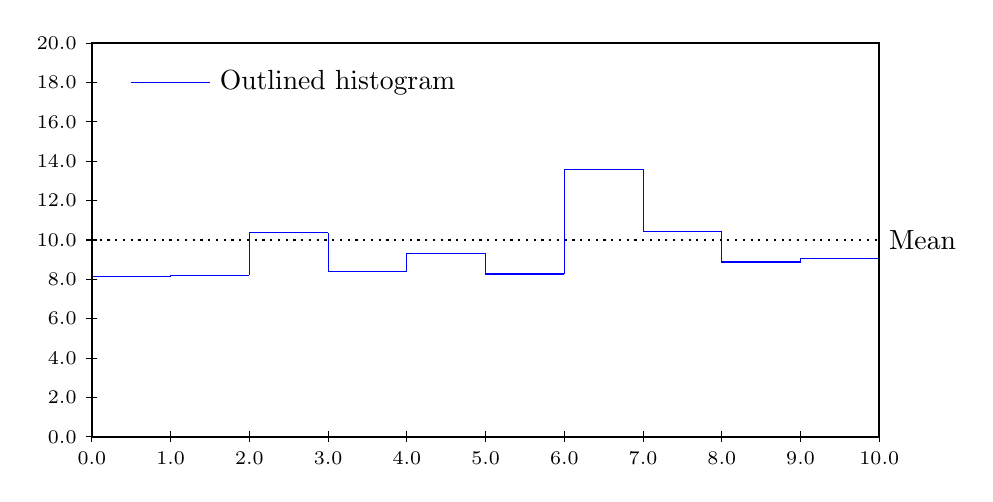
\begin{tikzpicture}
\begin{scope}[]
\clip (0,0) rectangle (10,5);
\begin{scope}[blue]
\draw[] (0.0,2.040753989729346) -- (1.0,2.040753989729346);
\draw (1.0,2.040753989729346) -- (1.0,2.0520371396851527) -- (2.0,2.0520371396851527);
\draw (2.0,2.0520371396851527) -- (2.0,2.589490136587087) -- (3.0,2.589490136587087);
\draw (3.0,2.589490136587087) -- (3.0,2.10531930397396) -- (4.0,2.10531930397396);
\draw (4.0,2.10531930397396) -- (4.0,2.328047479221825) -- (5.0,2.328047479221825);
\draw (5.0,2.328047479221825) -- (5.0,2.067390163042384) -- (6.0,2.067390163042384);
\draw (6.0,2.067390163042384) -- (6.0,3.3961419895360887) -- (7.0,3.3961419895360887);
\draw (7.0,3.3961419895360887) -- (7.0,2.6085288458106475) -- (8.0,2.6085288458106475);
\draw (8.0,2.6085288458106475) -- (8.0,2.2210174657245827) -- (9.0,2.2210174657245827);
\draw (9.0,2.2210174657245827) -- (9.0,2.2670683657782047) -- (10.0,2.2670683657782047);
\end{scope}
\end{scope}
\draw (0,0cm + 2pt) -- (0, 0cm -2pt) node[below] {\scriptsize{\num[round-mode=places,round-precision=1]{0}}};
\draw (1,0cm + 2pt) -- (1, 0cm -2pt) node[below] {\scriptsize{\num[round-mode=places,round-precision=1]{1}}};
\draw (2,0cm + 2pt) -- (2, 0cm -2pt) node[below] {\scriptsize{\num[round-mode=places,round-precision=1]{2}}};
\draw (3,0cm + 2pt) -- (3, 0cm -2pt) node[below] {\scriptsize{\num[round-mode=places,round-precision=1]{3}}};
\draw (4,0cm + 2pt) -- (4, 0cm -2pt) node[below] {\scriptsize{\num[round-mode=places,round-precision=1]{4}}};
\draw (5,0cm + 2pt) -- (5, 0cm -2pt) node[below] {\scriptsize{\num[round-mode=places,round-precision=1]{5}}};
\draw (6,0cm + 2pt) -- (6, 0cm -2pt) node[below] {\scriptsize{\num[round-mode=places,round-precision=1]{6}}};
\draw (7,0cm + 2pt) -- (7, 0cm -2pt) node[below] {\scriptsize{\num[round-mode=places,round-precision=1]{7}}};
\draw (8,0cm + 2pt) -- (8, 0cm -2pt) node[below] {\scriptsize{\num[round-mode=places,round-precision=1]{8}}};
\draw (9,0cm + 2pt) -- (9, 0cm -2pt) node[below] {\scriptsize{\num[round-mode=places,round-precision=1]{9}}};
\draw (10,0cm + 2pt) -- (10, 0cm -2pt) node[below] {\scriptsize{\num[round-mode=places,round-precision=1]{10}}};
\draw (0cm + 2pt,0.    ) -- (0cm-2pt,0.    ) node[left] {\scriptsize{\num[round-mode=places,round-precision=1]{0}}};
\draw (0cm + 2pt,0.5    ) -- (0cm-2pt,0.5    ) node[left] {\scriptsize{\num[round-mode=places,round-precision=1]{2}}};
\draw (0cm + 2pt,1.    ) -- (0cm-2pt,1.    ) node[left] {\scriptsize{\num[round-mode=places,round-precision=1]{4}}};
\draw (0cm + 2pt,1.5    ) -- (0cm-2pt,1.5    ) node[left] {\scriptsize{\num[round-mode=places,round-precision=1]{6}}};
\draw (0cm + 2pt,2.    ) -- (0cm-2pt,2.    ) node[left] {\scriptsize{\num[round-mode=places,round-precision=1]{8}}};
\draw (0cm + 2pt,2.5    ) -- (0cm-2pt,2.5    ) node[left] {\scriptsize{\num[round-mode=places,round-precision=1]{10}}};
\draw (0cm + 2pt,3.    ) -- (0cm-2pt,3.    ) node[left] {\scriptsize{\num[round-mode=places,round-precision=1]{12}}};
\draw (0cm + 2pt,3.5    ) -- (0cm-2pt,3.5    ) node[left] {\scriptsize{\num[round-mode=places,round-precision=1]{14}}};
\draw (0cm + 2pt,4.    ) -- (0cm-2pt,4.    ) node[left] {\scriptsize{\num[round-mode=places,round-precision=1]{16}}};
\draw (0cm + 2pt,4.5    ) -- (0cm-2pt,4.5    ) node[left] {\scriptsize{\num[round-mode=places,round-precision=1]{18}}};
\draw (0cm + 2pt,5.    ) -- (0cm-2pt,5.    ) node[left] {\scriptsize{\num[round-mode=places,round-precision=1]{20}}};
\draw[thick] (0,0) rectangle (10,5);
\draw[thick,dotted] (0.0,2.5) -- (10.0,2.5);
\node[right] at (10.0,2.5) {Mean};
\draw[blue] (0.5,4.5) -- (1.5,4.5);
\node[right,] at (1.5,4.5) {Outlined histogram};
\end{tikzpicture}
%%% Local Variables: 
%%% mode: latex 
%%% TeX-master: "master" 
%%% End:


  \caption{Basic histogram}
\end{figure}

\begin{figure}[H]
  \centering
  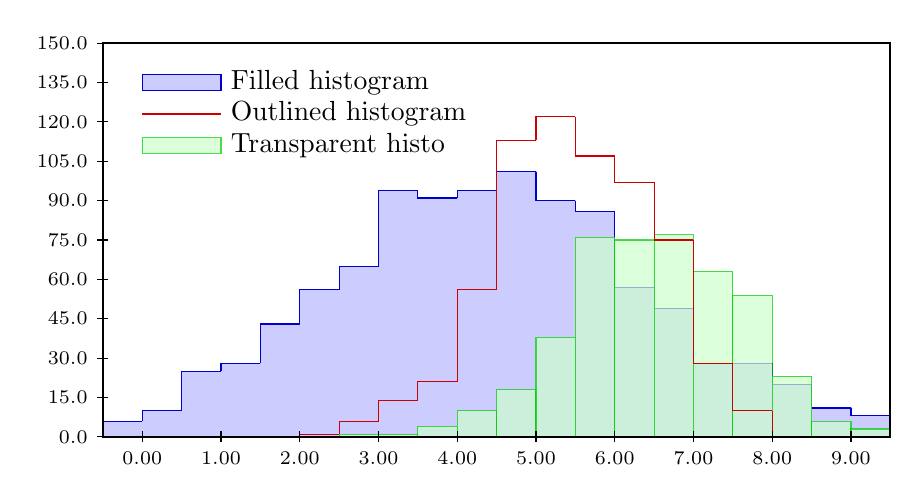
\begin{tikzpicture}
\begin{scope}[]
\clip (0,0) rectangle (10,5);
\begin{scope}[draw=blue!20,fill=blue!20]
\filldraw[] (0.0,0.0) -- (0.0,0.2) -- (0.5,0.2) -- (0.5,0.0);
\filldraw[] (0.5,0.0) -- (0.5,0.33333334) -- (1.0,0.33333334) -- (1.0,0.0);
\filldraw[] (1.0,0.0) -- (1.0,0.8333333) -- (1.5,0.8333333) -- (1.5,0.0);
\filldraw[] (1.5,0.0) -- (1.5,0.93333334) -- (2.0,0.93333334) -- (2.0,0.0);
\filldraw[] (2.0,0.0) -- (2.0,1.4333333) -- (2.5,1.4333333) -- (2.5,0.0);
\filldraw[] (2.5,0.0) -- (2.5,1.8666667) -- (3.0,1.8666667) -- (3.0,0.0);
\filldraw[] (3.0,0.0) -- (3.0,2.1666667) -- (3.5,2.1666667) -- (3.5,0.0);
\filldraw[] (3.5,0.0) -- (3.5,3.1333334) -- (4.0,3.1333334) -- (4.0,0.0);
\filldraw[] (4.0,0.0) -- (4.0,3.0333333) -- (4.5,3.0333333) -- (4.5,0.0);
\filldraw[] (4.5,0.0) -- (4.5,3.1333334) -- (5.0,3.1333334) -- (5.0,0.0);
\filldraw[] (5.0,0.0) -- (5.0,3.3666666) -- (5.5,3.3666666) -- (5.5,0.0);
\filldraw[] (5.5,0.0) -- (5.5,3.0) -- (6.0,3.0) -- (6.0,0.0);
\filldraw[] (6.0,0.0) -- (6.0,2.8666666) -- (6.5,2.8666666) -- (6.5,0.0);
\filldraw[] (6.5,0.0) -- (6.5,1.9) -- (7.0,1.9) -- (7.0,0.0);
\filldraw[] (7.0,0.0) -- (7.0,1.6333333) -- (7.5,1.6333333) -- (7.5,0.0);
\filldraw[] (7.5,0.0) -- (7.5,0.93333334) -- (8.0,0.93333334) -- (8.0,0.0);
\filldraw[] (8.0,0.0) -- (8.0,0.93333334) -- (8.5,0.93333334) -- (8.5,0.0);
\filldraw[] (8.5,0.0) -- (8.5,0.6666667) -- (9.0,0.6666667) -- (9.0,0.0);
\filldraw[] (9.0,0.0) -- (9.0,0.36666667) -- (9.5,0.36666667) -- (9.5,0.0);
\filldraw[] (9.5,0.0) -- (9.5,0.26666668) -- (10.0,0.26666668) -- (10.0,0.0);
\end{scope}
\begin{scope}[blue!80!black]
\draw[] (0.0,0.2) -- (0.5,0.2);
\draw (0.5,0.2) -- (0.5,0.33333334) -- (1.0,0.33333334);
\draw (1.0,0.33333334) -- (1.0,0.8333333) -- (1.5,0.8333333);
\draw (1.5,0.8333333) -- (1.5,0.93333334) -- (2.0,0.93333334);
\draw (2.0,0.93333334) -- (2.0,1.4333333) -- (2.5,1.4333333);
\draw (2.5,1.4333333) -- (2.5,1.8666667) -- (3.0,1.8666667);
\draw (3.0,1.8666667) -- (3.0,2.1666667) -- (3.5,2.1666667);
\draw (3.5,2.1666667) -- (3.5,3.1333334) -- (4.0,3.1333334);
\draw (4.0,3.1333334) -- (4.0,3.0333333) -- (4.5,3.0333333);
\draw (4.5,3.0333333) -- (4.5,3.1333334) -- (5.0,3.1333334);
\draw (5.0,3.1333334) -- (5.0,3.3666666) -- (5.5,3.3666666);
\draw (5.5,3.3666666) -- (5.5,3.0) -- (6.0,3.0);
\draw (6.0,3.0) -- (6.0,2.8666666) -- (6.5,2.8666666);
\draw (6.5,2.8666666) -- (6.5,1.9) -- (7.0,1.9);
\draw (7.0,1.9) -- (7.0,1.6333333) -- (7.5,1.6333333);
\draw (7.5,1.6333333) -- (7.5,0.93333334) -- (8.0,0.93333334);
\draw (8.0,0.93333334) -- (8.0,0.93333334) -- (8.5,0.93333334);
\draw (8.5,0.93333334) -- (8.5,0.6666667) -- (9.0,0.6666667);
\draw (9.0,0.6666667) -- (9.0,0.36666667) -- (9.5,0.36666667);
\draw (9.5,0.36666667) -- (9.5,0.26666668) -- (10.0,0.26666668);
\end{scope}
\begin{scope}[opacity=0.7,draw=green!80!black,fill=green!20]
\filldraw[] (0.0,0.0) -- (0.0,0.0) -- (0.5,0.0) -- (0.5,0.0);
\filldraw[] (0.5,0.0) -- (0.5,0.0) -- (1.0,0.0) -- (1.0,0.0);
\filldraw[] (1.0,0.0) -- (1.0,0.0) -- (1.5,0.0) -- (1.5,0.0);
\filldraw[] (1.5,0.0) -- (1.5,0.0) -- (2.0,0.0) -- (2.0,0.0);
\filldraw[] (2.0,0.0) -- (2.0,0.0) -- (2.5,0.0) -- (2.5,0.0);
\filldraw[] (2.5,0.0) -- (2.5,0.0) -- (3.0,0.0) -- (3.0,0.0);
\filldraw[] (3.0,0.0) -- (3.0,0.033333335) -- (3.5,0.033333335) -- (3.5,0.0);
\filldraw[] (3.5,0.0) -- (3.5,0.033333335) -- (4.0,0.033333335) -- (4.0,0.0);
\filldraw[] (4.0,0.0) -- (4.0,0.13333334) -- (4.5,0.13333334) -- (4.5,0.0);
\filldraw[] (4.5,0.0) -- (4.5,0.33333334) -- (5.0,0.33333334) -- (5.0,0.0);
\filldraw[] (5.0,0.0) -- (5.0,0.6) -- (5.5,0.6) -- (5.5,0.0);
\filldraw[] (5.5,0.0) -- (5.5,1.2666667) -- (6.0,1.2666667) -- (6.0,0.0);
\filldraw[] (6.0,0.0) -- (6.0,2.5333333) -- (6.5,2.5333333) -- (6.5,0.0);
\filldraw[] (6.5,0.0) -- (6.5,2.5) -- (7.0,2.5) -- (7.0,0.0);
\filldraw[] (7.0,0.0) -- (7.0,2.5666666) -- (7.5,2.5666666) -- (7.5,0.0);
\filldraw[] (7.5,0.0) -- (7.5,2.1) -- (8.0,2.1) -- (8.0,0.0);
\filldraw[] (8.0,0.0) -- (8.0,1.8) -- (8.5,1.8) -- (8.5,0.0);
\filldraw[] (8.5,0.0) -- (8.5,0.76666665) -- (9.0,0.76666665) -- (9.0,0.0);
\filldraw[] (9.0,0.0) -- (9.0,0.2) -- (9.5,0.2) -- (9.5,0.0);
\filldraw[] (9.5,0.0) -- (9.5,0.1) -- (10.0,0.1) -- (10.0,0.0);
\end{scope}
\begin{scope}[red!80!black]
\draw[] (0.0,0.0) -- (0.5,0.0);
\draw (0.5,0.0) -- (0.5,0.0) -- (1.0,0.0);
\draw (1.0,0.0) -- (1.0,0.0) -- (1.5,0.0);
\draw (1.5,0.0) -- (1.5,0.0) -- (2.0,0.0);
\draw (2.0,0.0) -- (2.0,0.0) -- (2.5,0.0);
\draw (2.5,0.0) -- (2.5,0.033333335) -- (3.0,0.033333335);
\draw (3.0,0.033333335) -- (3.0,0.2) -- (3.5,0.2);
\draw (3.5,0.2) -- (3.5,0.46666667) -- (4.0,0.46666667);
\draw (4.0,0.46666667) -- (4.0,0.7) -- (4.5,0.7);
\draw (4.5,0.7) -- (4.5,1.8666667) -- (5.0,1.8666667);
\draw (5.0,1.8666667) -- (5.0,3.7666667) -- (5.5,3.7666667);
\draw (5.5,3.7666667) -- (5.5,4.0666666) -- (6.0,4.0666666);
\draw (6.0,4.0666666) -- (6.0,3.5666666) -- (6.5,3.5666666);
\draw (6.5,3.5666666) -- (6.5,3.2333333) -- (7.0,3.2333333);
\draw (7.0,3.2333333) -- (7.0,2.5) -- (7.5,2.5);
\draw (7.5,2.5) -- (7.5,0.93333334) -- (8.0,0.93333334);
\draw (8.0,0.93333334) -- (8.0,0.33333334) -- (8.5,0.33333334);
\draw (8.5,0.33333334) -- (8.5,0.0) -- (9.0,0.0);
\draw (9.0,0.0) -- (9.0,0.0) -- (9.5,0.0);
\draw (9.5,0.0) -- (9.5,0.0) -- (10.0,0.0);
\end{scope}
\end{scope}
\draw (0.5,0cm + 2pt) -- (0.5, 0cm -2pt) node[below] {\scriptsize{\num[round-mode=places,round-precision=2]{0}}};
\draw (1.5,0cm + 2pt) -- (1.5, 0cm -2pt) node[below] {\scriptsize{\num[round-mode=places,round-precision=2]{1}}};
\draw (2.5,0cm + 2pt) -- (2.5, 0cm -2pt) node[below] {\scriptsize{\num[round-mode=places,round-precision=2]{2}}};
\draw (3.5,0cm + 2pt) -- (3.5, 0cm -2pt) node[below] {\scriptsize{\num[round-mode=places,round-precision=2]{3}}};
\draw (4.5,0cm + 2pt) -- (4.5, 0cm -2pt) node[below] {\scriptsize{\num[round-mode=places,round-precision=2]{4}}};
\draw (5.5,0cm + 2pt) -- (5.5, 0cm -2pt) node[below] {\scriptsize{\num[round-mode=places,round-precision=2]{5}}};
\draw (6.5,0cm + 2pt) -- (6.5, 0cm -2pt) node[below] {\scriptsize{\num[round-mode=places,round-precision=2]{6}}};
\draw (7.5,0cm + 2pt) -- (7.5, 0cm -2pt) node[below] {\scriptsize{\num[round-mode=places,round-precision=2]{7}}};
\draw (8.5,0cm + 2pt) -- (8.5, 0cm -2pt) node[below] {\scriptsize{\num[round-mode=places,round-precision=2]{8}}};
\draw (9.5,0cm + 2pt) -- (9.5, 0cm -2pt) node[below] {\scriptsize{\num[round-mode=places,round-precision=2]{9}}};
\draw (0cm + 2pt,0.    ) -- (0cm-2pt,0.    ) node[left] {\scriptsize{\num[round-mode=places,round-precision=1]{0}}};
\draw (0cm + 2pt,0.5    ) -- (0cm-2pt,0.5    ) node[left] {\scriptsize{\num[round-mode=places,round-precision=1]{15}}};
\draw (0cm + 2pt,1.    ) -- (0cm-2pt,1.    ) node[left] {\scriptsize{\num[round-mode=places,round-precision=1]{30}}};
\draw (0cm + 2pt,1.5    ) -- (0cm-2pt,1.5    ) node[left] {\scriptsize{\num[round-mode=places,round-precision=1]{45}}};
\draw (0cm + 2pt,2.    ) -- (0cm-2pt,2.    ) node[left] {\scriptsize{\num[round-mode=places,round-precision=1]{60}}};
\draw (0cm + 2pt,2.5    ) -- (0cm-2pt,2.5    ) node[left] {\scriptsize{\num[round-mode=places,round-precision=1]{75}}};
\draw (0cm + 2pt,3.    ) -- (0cm-2pt,3.    ) node[left] {\scriptsize{\num[round-mode=places,round-precision=1]{90}}};
\draw (0cm + 2pt,3.5    ) -- (0cm-2pt,3.5    ) node[left] {\scriptsize{\num[round-mode=places,round-precision=1]{105}}};
\draw (0cm + 2pt,4.    ) -- (0cm-2pt,4.    ) node[left] {\scriptsize{\num[round-mode=places,round-precision=1]{120}}};
\draw (0cm + 2pt,4.5    ) -- (0cm-2pt,4.5    ) node[left] {\scriptsize{\num[round-mode=places,round-precision=1]{135}}};
\draw (0cm + 2pt,5.    ) -- (0cm-2pt,5.    ) node[left] {\scriptsize{\num[round-mode=places,round-precision=1]{150}}};
\draw[thick] (0,0) rectangle (10,5);
\draw[draw=blue!20,fill=blue!20] (0.5,4.4) rectangle (1.5,4.6);
\draw[blue!80!black] (0.5,4.4) rectangle (1.5,4.6);
\node[right,] at (1.5,4.5) {Filled histogram};
\draw[red!80!black] (0.5,4.1) -- (1.5,4.1);
\node[right,] at (1.5,4.1) {Outlined histogram};
\draw[opacity=0.7,draw=green!80!black,fill=green!20] (0.5,3.6000001) rectangle (1.5,3.8);
\node[right,] at (1.5,3.7) {Transparent histo};
\end{tikzpicture}
%%% Local Variables: 
%%% mode: latex 
%%% TeX-master: "master" 
%%% End:


  \caption{Three histograms in the same figure}
\end{figure}

\section{Fitting with Levenberg marquart algorithm and splines}
\label{sec:LMA}

\begin{figure}[H]
  \centering
  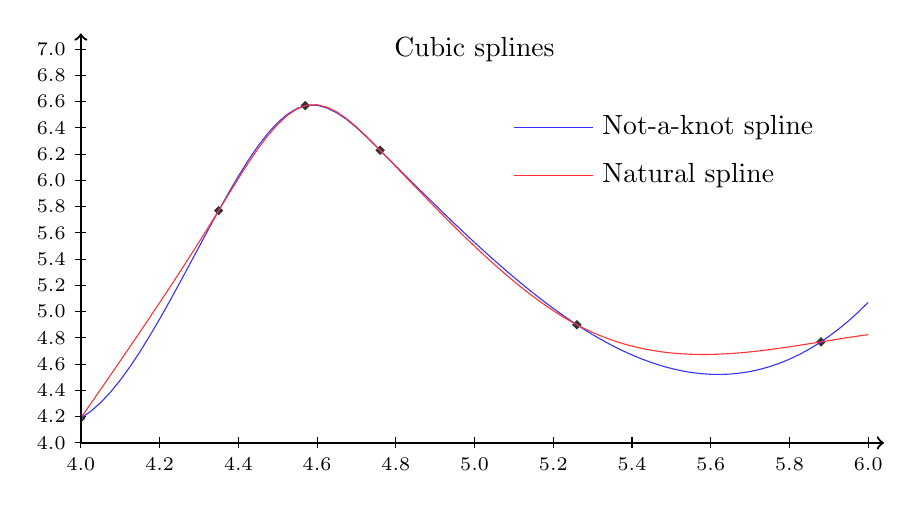
\begin{tikzpicture}
\draw (0.0,0cm + 2pt) -- (0.0, 0cm -2pt) node[below] {\scriptsize{\num[round-mode=places,round-precision=1]{4.0}}};
\draw (0.99999905,0cm + 2pt) -- (0.99999905, 0cm -2pt) node[below] {\scriptsize{\num[round-mode=places,round-precision=1]{4.2}}};
\draw (2.0000005,0cm + 2pt) -- (2.0000005, 0cm -2pt) node[below] {\scriptsize{\num[round-mode=places,round-precision=1]{4.4}}};
\draw (2.9999995,0cm + 2pt) -- (2.9999995, 0cm -2pt) node[below] {\scriptsize{\num[round-mode=places,round-precision=1]{4.6}}};
\draw (4.000001,0cm + 2pt) -- (4.000001, 0cm -2pt) node[below] {\scriptsize{\num[round-mode=places,round-precision=1]{4.8}}};
\draw (5.0,0cm + 2pt) -- (5.0, 0cm -2pt) node[below] {\scriptsize{\num[round-mode=places,round-precision=1]{5.0}}};
\draw (5.999999,0cm + 2pt) -- (5.999999, 0cm -2pt) node[below] {\scriptsize{\num[round-mode=places,round-precision=1]{5.2}}};
\draw (7.0000005,0cm + 2pt) -- (7.0000005, 0cm -2pt) node[below] {\scriptsize{\num[round-mode=places,round-precision=1]{5.4}}};
\draw (7.9999995,0cm + 2pt) -- (7.9999995, 0cm -2pt) node[below] {\scriptsize{\num[round-mode=places,round-precision=1]{5.6}}};
\draw (9.000001,0cm + 2pt) -- (9.000001, 0cm -2pt) node[below] {\scriptsize{\num[round-mode=places,round-precision=1]{5.8}}};
\draw (10.0,0cm + 2pt) -- (10.0, 0cm -2pt) node[below] {\scriptsize{\num[round-mode=places,round-precision=1]{6.0}}};
\draw (0cm + 2pt,0.    ) -- (0cm-2pt,0.    ) node[left] {\scriptsize{\num[round-mode=places,round-precision=1]{4.0}}};
\draw (0cm + 2pt,0.33333302    ) -- (0cm-2pt,0.33333302    ) node[left] {\scriptsize{\num[round-mode=places,round-precision=1]{4.2}}};
\draw (0cm + 2pt,0.6666668    ) -- (0cm-2pt,0.6666668    ) node[left] {\scriptsize{\num[round-mode=places,round-precision=1]{4.4}}};
\draw (0cm + 2pt,0.9999998    ) -- (0cm-2pt,0.9999998    ) node[left] {\scriptsize{\num[round-mode=places,round-precision=1]{4.6}}};
\draw (0cm + 2pt,1.3333336    ) -- (0cm-2pt,1.3333336    ) node[left] {\scriptsize{\num[round-mode=places,round-precision=1]{4.8}}};
\draw (0cm + 2pt,1.6666666    ) -- (0cm-2pt,1.6666666    ) node[left] {\scriptsize{\num[round-mode=places,round-precision=1]{5.0}}};
\draw (0cm + 2pt,1.9999996    ) -- (0cm-2pt,1.9999996    ) node[left] {\scriptsize{\num[round-mode=places,round-precision=1]{5.2}}};
\draw (0cm + 2pt,2.3333335    ) -- (0cm-2pt,2.3333335    ) node[left] {\scriptsize{\num[round-mode=places,round-precision=1]{5.4}}};
\draw (0cm + 2pt,2.6666665    ) -- (0cm-2pt,2.6666665    ) node[left] {\scriptsize{\num[round-mode=places,round-precision=1]{5.6}}};
\draw (0cm + 2pt,3.0000002    ) -- (0cm-2pt,3.0000002    ) node[left] {\scriptsize{\num[round-mode=places,round-precision=1]{5.8}}};
\draw (0cm + 2pt,3.3333333    ) -- (0cm-2pt,3.3333333    ) node[left] {\scriptsize{\num[round-mode=places,round-precision=1]{6.0}}};
\draw (0cm + 2pt,3.6666663    ) -- (0cm-2pt,3.6666663    ) node[left] {\scriptsize{\num[round-mode=places,round-precision=1]{6.2}}};
\draw (0cm + 2pt,4.    ) -- (0cm-2pt,4.    ) node[left] {\scriptsize{\num[round-mode=places,round-precision=1]{6.4}}};
\draw (0cm + 2pt,4.333334    ) -- (0cm-2pt,4.333334    ) node[left] {\scriptsize{\num[round-mode=places,round-precision=1]{6.6000004}}};
\draw (0cm + 2pt,4.666667    ) -- (0cm-2pt,4.666667    ) node[left] {\scriptsize{\num[round-mode=places,round-precision=1]{6.8}}};
\draw (0cm + 2pt,5.    ) -- (0cm-2pt,5.    ) node[left] {\scriptsize{\num[round-mode=places,round-precision=1]{7.0}}};
\node[] at (5.0,5.0) {Cubic splines};
\begin{scope}[]
\clip (0,0) rectangle (10,5);
\node at (0.0,0.316666654083465) [draw=black!80,fill=black!80,diamond,inner sep=0pt,minimum width =3pt,minimum height=3pt] {}; 
\node at (1.7499999739229666,2.949999882777536) [draw=black!80,fill=black!80,diamond,inner sep=0pt,minimum width =3pt,minimum height=3pt] {}; 
\node at (2.8499999575316926,4.283333163128966) [draw=black!80,fill=black!80,diamond,inner sep=0pt,minimum width =3pt,minimum height=3pt] {}; 
\node at (3.799999943375587,3.716666518979609) [draw=black!80,fill=black!80,diamond,inner sep=0pt,minimum width =3pt,minimum height=3pt] {}; 
\node at (6.299999906122685,1.4999999403953581) [draw=black!80,fill=black!80,diamond,inner sep=0pt,minimum width =3pt,minimum height=3pt] {}; 
\node at (9.399999859929085,1.2833332823382497) [draw=black!80,fill=black!80,diamond,inner sep=0pt,minimum width =3pt,minimum height=3pt] {}; 
\begin{scope}[blue!80]
\draw[] (-2.4999999627470975,7.7943914926862305) -- (-2.374999964609743,6.85271188831033);
\draw[] (-2.374999964609743,6.85271188831033) -- (-2.2499999664723886,5.985369091033453);
\draw[] (-2.2499999664723886,5.985369091033453) -- (-2.124999968335032,5.189934920066197);
\draw[] (-2.124999968335032,5.189934920066197) -- (-1.9999999701976776,4.4639811946192065);
\draw[] (-1.9999999701976776,4.4639811946192065) -- (-1.8749999720603232,3.8050797339030833);
\draw[] (-1.8749999720603232,3.8050797339030833) -- (-1.7499999739229688,3.2108023571284394);
\draw[] (-1.7499999739229688,3.2108023571284394) -- (-1.6249999757856144,2.6787208835058913);
\draw[] (-1.6249999757856144,2.6787208835058913) -- (-1.4999999776482578,2.206407132246049);
\draw[] (-1.4999999776482578,2.206407132246049) -- (-1.3749999795109031,1.7914329225595402);
\draw[] (-1.3749999795109031,1.7914329225595402) -- (-1.2499999813735487,1.431370073656974);
\draw[] (-1.2499999813735487,1.431370073656974) -- (-1.1249999832361943,1.1237904047489642);
\draw[] (-1.1249999832361943,1.1237904047489642) -- (-0.9999999850988399,0.8662657350461275);
\draw[] (-0.9999999850988399,0.8662657350461275) -- (-0.8749999869614833,0.6563678837590736);
\draw[] (-0.8749999869614833,0.6563678837590736) -- (-0.7499999888241289,0.49166867009842874);
\draw[] (-0.7499999888241289,0.49166867009842874) -- (-0.6249999906867744,0.36973991327480216);
\draw[] (-0.6249999906867744,0.36973991327480216) -- (-0.49999999254941996,0.2881534324988066);
\draw[] (-0.49999999254941996,0.2881534324988066) -- (-0.3749999944120655,0.24448104698106043);
\draw[] (-0.3749999944120655,0.24448104698106043) -- (-0.24999999627470887,0.23629457593217776);
\draw[] (-0.24999999627470887,0.23629457593217776) -- (-0.12499999813735443,0.26116583856277414);
\draw[] (-0.12499999813735443,0.26116583856277414) -- (0.0,0.316666654083465);
\draw[] (0.0,0.316666654083465) -- (0.12499999813735665,0.4003688417048675);
\draw[] (0.12499999813735665,0.4003688417048675) -- (0.24999999627470887,0.5098442206375896);
\draw[] (0.24999999627470887,0.5098442206375896) -- (0.3749999944120655,0.6426646100922557);
\draw[] (0.3749999944120655,0.6426646100922557) -- (0.49999999254941774,0.7964018292794712);
\draw[] (0.49999999254941774,0.7964018292794712) -- (0.6249999906867744,0.9686276974098632);
\draw[] (0.6249999906867744,0.9686276974098632) -- (0.749999988824131,1.1569140336940429);
\draw[] (0.749999988824131,1.1569140336940429) -- (0.8749999869614833,1.358832657342614);
\draw[] (0.8749999869614833,1.358832657342614) -- (0.9999999850988399,1.5719553875662082);
\draw[] (0.9999999850988399,1.5719553875662082) -- (1.124999983236192,1.793854043575428);
\draw[] (1.124999983236192,1.793854043575428) -- (1.2499999813735487,2.0221004445808974);
\draw[] (1.2499999813735487,2.0221004445808974) -- (1.3749999795109054,2.2542664097932303);
\draw[] (1.3749999795109054,2.2542664097932303) -- (1.4999999776482578,2.487923758423034);
\draw[] (1.4999999776482578,2.487923758423034) -- (1.6249999757856144,2.7206443096809374);
\draw[] (1.6249999757856144,2.7206443096809374) -- (1.7499999739229666,2.9499998827775373);
\draw[] (1.7499999739229666,2.9499998827775373) -- (1.8749999720603232,3.1733231579063315);
\draw[] (1.8749999720603232,3.1733231579063315) -- (1.9999999701976798,3.386990259192244);
\draw[] (1.9999999701976798,3.386990259192244) -- (2.124999968335032,3.5871381717430655);
\draw[] (2.124999968335032,3.5871381717430655) -- (2.2499999664723886,3.7699038806666065);
\draw[] (2.2499999664723886,3.7699038806666065) -- (2.374999964609741,3.931424371070651);
\draw[] (2.374999964609741,3.931424371070651) -- (2.4999999627470975,4.06783662806301);
\draw[] (2.4999999627470975,4.06783662806301) -- (2.624999960884454,4.17527763675147);
\draw[] (2.624999960884454,4.17527763675147) -- (2.7499999590218063,4.24988438224383);
\draw[] (2.7499999590218063,4.24988438224383) -- (2.874999957159163,4.287805970399012);
\draw[] (2.874999957159163,4.287805970399012) -- (2.9999999552965155,4.287761106314666);
\draw[] (2.9999999552965155,4.287761106314666) -- (3.124999953433872,4.254201610371051);
\draw[] (3.124999953433872,4.254201610371051) -- (3.249999951571229,4.192355031020499);
\draw[] (3.249999951571229,4.192355031020499) -- (3.374999949708581,4.1074489167153505);
\draw[] (3.374999949708581,4.1074489167153505) -- (3.4999999478459376,4.004710815907926);
\draw[] (3.4999999478459376,4.004710815907926) -- (3.62499994598329,3.88936827705057);
\draw[] (3.62499994598329,3.88936827705057) -- (3.7499999441206464,3.766648848595603);
\draw[] (3.7499999441206464,3.766648848595603) -- (3.874999942258003,3.641599909911412);
\draw[] (3.874999942258003,3.641599909911412) -- (3.9999999403953552,3.5165729770361955);
\draw[] (3.9999999403953552,3.5165729770361955) -- (4.124999938532712,3.3918442850782133);
\draw[] (4.124999938532712,3.3918442850782133) -- (4.249999936670064,3.2676366857134576);
\draw[] (4.249999936670064,3.2676366857134576) -- (4.374999934807421,3.144173030617912);
\draw[] (4.374999934807421,3.144173030617912) -- (4.499999932944777,3.021676171467562);
\draw[] (4.499999932944777,3.021676171467562) -- (4.6249999310821295,2.9003689599384015);
\draw[] (4.6249999310821295,2.9003689599384015) -- (4.749999929219486,2.7804742477064077);
\draw[] (4.749999929219486,2.7804742477064077) -- (4.874999927356838,2.6622148864475754);
\draw[] (4.874999927356838,2.6622148864475754) -- (4.999999925494195,2.545813727837884);
\draw[] (4.999999925494195,2.545813727837884) -- (5.1249999236315515,2.4314936235533224);
\draw[] (5.1249999236315515,2.4314936235533224) -- (5.249999921768904,2.3194774252698838);
\draw[] (5.249999921768904,2.3194774252698838) -- (5.37499991990626,2.2099879846635475);
\draw[] (5.37499991990626,2.2099879846635475) -- (5.4999999180436125,2.103248153410304);
\draw[] (5.4999999180436125,2.103248153410304) -- (5.624999916180969,1.9994807831861359);
\draw[] (5.624999916180969,1.9994807831861359) -- (5.749999914318326,1.8989087256670316);
\draw[] (5.749999914318326,1.8989087256670316) -- (5.874999912455678,1.8017548325289818);
\draw[] (5.874999912455678,1.8017548325289818) -- (5.999999910593035,1.708241955447969);
\draw[] (5.999999910593035,1.708241955447969) -- (6.124999908730388,1.6185929460999828);
\draw[] (6.124999908730388,1.6185929460999828) -- (6.249999906867744,1.533030656161004);
\draw[] (6.249999906867744,1.533030656161004) -- (6.374999905005101,1.451776384534055);
\draw[] (6.374999905005101,1.451776384534055) -- (6.499999903142453,1.3750281960377477);
\draw[] (6.499999903142453,1.3750281960377477) -- (6.62499990127981,1.3029662698464899);
\draw[] (6.62499990127981,1.3029662698464899) -- (6.749999899417162,1.2357703250538243);
\draw[] (6.749999899417162,1.2357703250538243) -- (6.874999897554519,1.173620080753285);
\draw[] (6.874999897554519,1.173620080753285) -- (6.999999895691875,1.116695256038412);
\draw[] (6.999999895691875,1.116695256038412) -- (7.124999893829227,1.0651755700027439);
\draw[] (7.124999893829227,1.0651755700027439) -- (7.249999891966584,1.0192407417398162);
\draw[] (7.249999891966584,1.0192407417398162) -- (7.374999890103936,0.9790704903431704);
\draw[] (7.374999890103936,0.9790704903431704) -- (7.499999888241293,0.944844534906336);
\draw[] (7.499999888241293,0.944844534906336) -- (7.6249998863786494,0.9167425945228603);
\draw[] (7.6249998863786494,0.9167425945228603) -- (7.749999884516006,0.8949443882862762);
\draw[] (7.749999884516006,0.8949443882862762) -- (7.874999882653358,0.879629635290119);
\draw[] (7.874999882653358,0.879629635290119) -- (7.9999998807907104,0.8709780546279331);
\draw[] (7.9999998807907104,0.8709780546279331) -- (8.124999878928067,0.8691693653932512);
\draw[] (8.124999878928067,0.8691693653932512) -- (8.249999877065424,0.8743832866796089);
\draw[] (8.249999877065424,0.8743832866796089) -- (8.37499987520278,0.8867995375805503);
\draw[] (8.37499987520278,0.8867995375805503) -- (8.499999873340133,0.9065978371896083);
\draw[] (8.499999873340133,0.9065978371896083) -- (8.624999871477485,0.9339579046003212);
\draw[] (8.624999871477485,0.9339579046003212) -- (8.749999869614841,0.9690594589062291);
\draw[] (8.749999869614841,0.9690594589062291) -- (8.874999867752198,1.0120822192008692);
\draw[] (8.874999867752198,1.0120822192008692) -- (8.999999865889555,1.0632059045777764);
\draw[] (8.999999865889555,1.0632059045777764) -- (9.124999864026908,1.12261023413049);
\draw[] (9.124999864026908,1.12261023413049) -- (9.249999862164259,1.190474926952545);
\draw[] (9.249999862164259,1.190474926952545) -- (9.374999860301616,1.2669797021374845);
\draw[] (9.374999860301616,1.2669797021374845) -- (9.499999858438972,1.3523042787788442);
\draw[] (9.499999858438972,1.3523042787788442) -- (9.624999856576329,1.4466283759701621);
\draw[] (9.624999856576329,1.4466283759701621) -- (9.749999854713682,1.5501317128049699);
\draw[] (9.749999854713682,1.5501317128049699) -- (9.874999852851033,1.6629940083768073);
\draw[] (9.874999852851033,1.6629940083768073) -- (9.99999985098839,1.7853949817792232);
\end{scope}
\begin{scope}[red!80]
\draw[] (-2.4999999627470975,-3.605941027545164) -- (-2.374999964609743,-3.38062413015895);
\draw[] (-2.374999964609743,-3.38062413015895) -- (-2.2499999664723886,-3.159797465588856);
\draw[] (-2.2499999664723886,-3.159797465588856) -- (-2.124999968335032,-2.943224705791926);
\draw[] (-2.124999968335032,-2.943224705791926) -- (-1.9999999701976776,-2.730669522725212);
\draw[] (-1.9999999701976776,-2.730669522725212) -- (-1.8749999720603232,-2.5218955883457586);
\draw[] (-1.8749999720603232,-2.5218955883457586) -- (-1.7499999739229688,-2.3166665746106103);
\draw[] (-1.7499999739229688,-2.3166665746106103) -- (-1.6249999757856144,-2.114746153476813);
\draw[] (-1.6249999757856144,-2.114746153476813) -- (-1.4999999776482578,-1.9158979969014112);
\draw[] (-1.4999999776482578,-1.9158979969014112) -- (-1.3749999795109031,-1.7198857768414577);
\draw[] (-1.3749999795109031,-1.7198857768414577) -- (-1.2499999813735487,-1.526473165253995);
\draw[] (-1.2499999813735487,-1.526473165253995) -- (-1.1249999832361943,-1.3354238340960685);
\draw[] (-1.1249999832361943,-1.3354238340960685) -- (-0.9999999850988399,-1.1465014553247257);
\draw[] (-0.9999999850988399,-1.1465014553247257) -- (-0.8749999869614833,-0.95946970089701);
\draw[] (-0.8749999869614833,-0.95946970089701) -- (-0.7499999888241289,-0.7740922427699727);
\draw[] (-0.7499999888241289,-0.7740922427699727) -- (-0.6249999906867744,-0.5901327529006577);
\draw[] (-0.6249999906867744,-0.5901327529006577) -- (-0.49999999254941996,-0.4073549032461111);
\draw[] (-0.49999999254941996,-0.4073549032461111) -- (-0.3749999944120655,-0.2255223657633807);
\draw[] (-0.3749999944120655,-0.2255223657633807) -- (-0.24999999627470887,-0.04439881240950658);
\draw[] (-0.24999999627470887,-0.04439881240950658) -- (-0.12499999813735443,0.1362520848584554);
\draw[] (-0.12499999813735443,0.1362520848584554) -- (0.0,0.316666654083465);
\draw[] (0.0,0.316666654083465) -- (0.12499999813735665,0.4970812233084776);
\draw[] (0.12499999813735665,0.4970812233084776) -- (0.24999999627470887,0.677732120576436);
\draw[] (0.24999999627470887,0.677732120576436) -- (0.3749999944120655,0.8588556739303093);
\draw[] (0.3749999944120655,0.8588556739303093) -- (0.49999999254941774,1.040688211413039);
\draw[] (0.49999999254941774,1.040688211413039) -- (0.6249999906867744,1.2234660610675885);
\draw[] (0.6249999906867744,1.2234660610675885) -- (0.749999988824131,1.4074255509369065);
\draw[] (0.749999988824131,1.4074255509369065) -- (0.8749999869614833,1.5928030090639387);
\draw[] (0.8749999869614833,1.5928030090639387) -- (0.9999999850988399,1.7798347634916558);
\draw[] (0.9999999850988399,1.7798347634916558) -- (1.124999983236192,1.9687571422629948);
\draw[] (1.124999983236192,1.9687571422629948) -- (1.2499999813735487,2.159806473420925);
\draw[] (1.2499999813735487,2.159806473420925) -- (1.3749999795109054,2.353219085008392);
\draw[] (1.3749999795109054,2.353219085008392) -- (1.4999999776482578,2.5492313050683406);
\draw[] (1.4999999776482578,2.5492313050683406) -- (1.6249999757856144,2.748079461643744);
\draw[] (1.6249999757856144,2.748079461643744) -- (1.7499999739229666,2.9499998827775373);
\draw[] (1.7499999739229666,2.9499998827775373) -- (1.8749999720603232,3.154329772046608);
\draw[] (1.8749999720603232,3.154329772046608) -- (1.9999999701976798,3.356809835163513);
\draw[] (1.9999999701976798,3.356809835163513) -- (2.124999968335032,3.552281653374717);
\draw[] (2.124999968335032,3.552281653374717) -- (2.2499999664723886,3.735586807926718);
\draw[] (2.2499999664723886,3.735586807926718) -- (2.374999964609741,3.9015668800659786);
\draw[] (2.374999964609741,3.9015668800659786) -- (2.4999999627470975,4.045063451038991);
\draw[] (2.4999999627470975,4.045063451038991) -- (2.624999960884454,4.160918102092223);
\draw[] (2.624999960884454,4.160918102092223) -- (2.7499999590218063,4.243972414472157);
\draw[] (2.7499999590218063,4.243972414472157) -- (2.874999957159163,4.289082111375187);
\draw[] (2.874999957159163,4.289082111375187) -- (2.9999999552965155,4.294101009379233);
\draw[] (2.9999999552965155,4.294101009379233) -- (3.124999953433872,4.263572067371012);
\draw[] (3.124999953433872,4.263572067371012) -- (3.249999951571229,4.202943329031665);
\draw[] (3.249999951571229,4.202943329031665) -- (3.374999949708581,4.117662838042336);
\draw[] (3.374999949708581,4.117662838042336) -- (3.4999999478459376,4.01317863808416);
\draw[] (3.4999999478459376,4.01317863808416) -- (3.62499994598329,3.8949387728382847);
\draw[] (3.62499994598329,3.8949387728382847) -- (3.7499999441206464,3.768391285985844);
\draw[] (3.7499999441206464,3.768391285985844) -- (3.874999942258003,3.6388018959505035);
\draw[] (3.874999942258003,3.6388018959505035) -- (3.9999999403953552,3.5087081950810326);
\draw[] (3.9999999403953552,3.5087081950810326) -- (4.124999938532712,3.3785476588715095);
\draw[] (4.124999938532712,3.3785476588715095) -- (4.249999936670064,3.248703740517511);
\draw[] (4.249999936670064,3.248703740517511) -- (4.374999934807421,3.1195598932146047);
\draw[] (4.374999934807421,3.1195598932146047) -- (4.499999932944777,2.9914995701583624);
\draw[] (4.499999932944777,2.9914995701583624) -- (4.6249999310821295,2.864906224544363);
\draw[] (4.6249999310821295,2.864906224544363) -- (4.749999929219486,2.740163309568167);
\draw[] (4.749999929219486,2.740163309568167) -- (4.874999927356838,2.617654278425355);
\draw[] (4.874999927356838,2.617654278425355) -- (4.999999925494195,2.497762584311492);
\draw[] (4.999999925494195,2.497762584311492) -- (5.1249999236315515,2.380871680422152);
\draw[] (5.1249999236315515,2.380871680422152) -- (5.249999921768904,2.267365019952912);
\draw[] (5.249999921768904,2.267365019952912) -- (5.37499991990626,2.157626056099335);
\draw[] (5.37499991990626,2.157626056099335) -- (5.4999999180436125,2.0520382420570016);
\draw[] (5.4999999180436125,2.0520382420570016) -- (5.624999916180969,1.9509850310214718);
\draw[] (5.624999916180969,1.9509850310214718) -- (5.749999914318326,1.8548498761883265);
\draw[] (5.749999914318326,1.8548498761883265) -- (5.874999912455678,1.764016230753138);
\draw[] (5.874999912455678,1.764016230753138) -- (5.999999910593035,1.6788675479114719);
\draw[] (5.999999910593035,1.6788675479114719) -- (6.124999908730388,1.5997872808589044);
\draw[] (6.124999908730388,1.5997872808589044) -- (6.249999906867744,1.5271588827910019);
\draw[] (6.249999906867744,1.5271588827910019) -- (6.374999905005101,1.4613418576961836);
\draw[] (6.374999905005101,1.4613418576961836) -- (6.499999903142453,1.4023373584631706);
\draw[] (6.499999903142453,1.4023373584631706) -- (6.62499990127981,1.3498706785945276);
\draw[] (6.62499990127981,1.3498706785945276) -- (6.749999899417162,1.3036600155314544);
\draw[] (6.749999899417162,1.3036600155314544) -- (6.874999897554519,1.2634235667151321);
\draw[] (6.874999897554519,1.2634235667151321) -- (6.999999895691875,1.2288795295867583);
\draw[] (6.999999895691875,1.2288795295867583) -- (7.124999893829227,1.1997461015875226);
\draw[] (7.124999893829227,1.1997461015875226) -- (7.249999891966584,1.175741480158612);
\draw[] (7.249999891966584,1.175741480158612) -- (7.374999890103936,1.1565838627412233);
\draw[] (7.374999890103936,1.1565838627412233) -- (7.499999888241293,1.1419914467765409);
\draw[] (7.499999888241293,1.1419914467765409) -- (7.6249998863786494,1.1316824297057606);
\draw[] (7.6249998863786494,1.1316824297057606) -- (7.749999884516006,1.1253750089700705);
\draw[] (7.749999884516006,1.1253750089700705) -- (7.874999882653358,1.1227873820106633);
\draw[] (7.874999882653358,1.1227873820106633) -- (7.9999998807907104,1.1236377462687277);
\draw[] (7.9999998807907104,1.1236377462687277) -- (8.124999878928067,1.127644299185455);
\draw[] (8.124999878928067,1.127644299185455) -- (8.249999877065424,1.1345252382020363);
\draw[] (8.249999877065424,1.1345252382020363) -- (8.37499987520278,1.143998760759663);
\draw[] (8.37499987520278,1.143998760759663) -- (8.499999873340133,1.155783064299525);
\draw[] (8.499999873340133,1.155783064299525) -- (8.624999871477485,1.1695963462628136);
\draw[] (8.624999871477485,1.1695963462628136) -- (8.749999869614841,1.1851568040907217);
\draw[] (8.749999869614841,1.1851568040907217) -- (8.874999867752198,1.2021826352244345);
\draw[] (8.874999867752198,1.2021826352244345) -- (8.999999865889555,1.220392037105148);
\draw[] (8.999999865889555,1.220392037105148) -- (9.124999864026908,1.2395032071740488);
\draw[] (9.124999864026908,1.2395032071740488) -- (9.249999862164259,1.2592343428723314);
\draw[] (9.249999862164259,1.2592343428723314) -- (9.374999860301616,1.2793036416411872);
\draw[] (9.374999860301616,1.2793036416411872) -- (9.499999858438972,1.2994293009218014);
\draw[] (9.499999858438972,1.2994293009218014) -- (9.624999856576329,1.3193295181553697);
\draw[] (9.624999856576329,1.3193295181553697) -- (9.749999854713682,1.3387224907830808);
\draw[] (9.749999854713682,1.3387224907830808) -- (9.874999852851033,1.3573264162461258);
\draw[] (9.874999852851033,1.3573264162461258) -- (9.99999985098839,1.3748594919856976);
\end{scope}
\end{scope}
\draw[blue!80] (5.5,4.0) -- (6.5,4.0);
\node[right,] at (6.5,4.0) {Not-a-knot spline};
\draw[red!80] (5.5,3.4) -- (6.5,3.4);
\node[right,] at (6.5,3.4) {Natural spline};
\draw[thick,->] (0.0,0.0) -- (10.2,0.0);
\draw[thick,->] (0.0,0.0) -- (0.0,5.2);
\end{tikzpicture}
%%% Local Variables: 
%%% mode: latex 
%%% TeX-master: "master" 
%%% End:


  \caption{Comparison of splines with different end point conditions.}
\end{figure}

\begin{figure}[H]
  \centering
  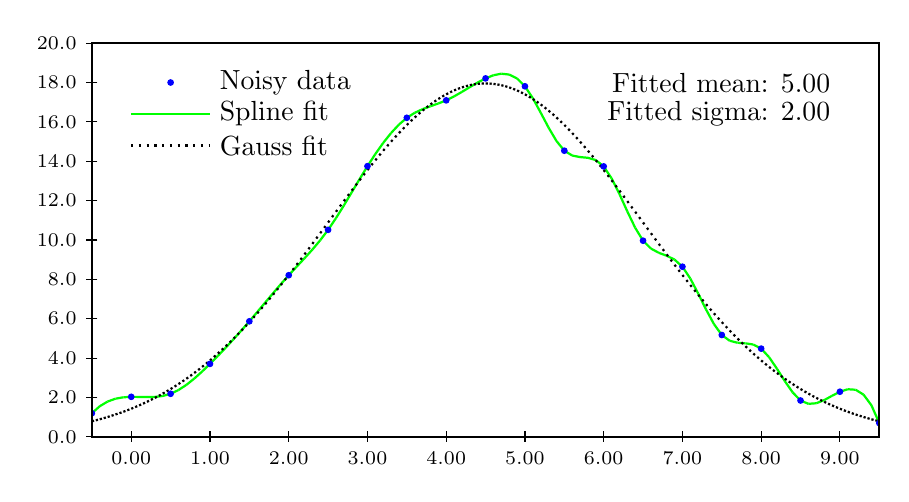
\begin{tikzpicture}
\begin{scope}[]
\clip (0,0) rectangle (10,5);
\begin{scope}[green,thick]
\draw[] (0.0,0.2998554191980206) -- (0.1,0.3886769723521621);
\draw[] (0.1,0.3886769723521621) -- (0.2,0.4483013692841718);
\draw[] (0.2,0.4483013692841718) -- (0.3,0.48433430438467895);
\draw[] (0.3,0.48433430438467895) -- (0.4,0.5023814720443124);
\draw[] (0.4,0.5023814720443124) -- (0.5,0.508048566653701);
\draw[] (0.5,0.508048566653701) -- (0.6,0.506941282603474);
\draw[] (0.6,0.506941282603474) -- (0.7,0.5046653142842601);
\draw[] (0.7,0.5046653142842601) -- (0.8,0.5068263560866882);
\draw[] (0.8,0.5068263560866882) -- (0.9,0.5190301024013876);
\draw[] (0.9,0.5190301024013876) -- (1.0,0.5468822476189868);
\draw[] (1.0,0.5468822476189868) -- (1.1,0.5944637212948228);
\draw[] (1.1,0.5944637212948228) -- (1.2,0.6597563936430622);
\draw[] (1.2,0.6597563936430622) -- (1.3,0.7392173700425795);
\draw[] (1.3,0.7392173700425795) -- (1.4,0.8293037558722491);
\draw[] (1.4,0.8293037558722491) -- (1.5,0.9264726565109458);
\draw[] (1.5,0.9264726565109458) -- (1.6,1.0277622403859983);
\draw[] (1.6,1.0277622403859983) -- (1.7,1.1325349281185535);
\draw[] (1.7,1.1325349281185535) -- (1.8,1.2407342033782138);
\draw[] (1.8,1.2407342033782138) -- (1.9,1.3523035498345806);
\draw[] (1.9,1.3523035498345806) -- (2.0,1.4671864511572559);
\draw[] (2.0,1.4671864511572559) -- (2.1,1.5850318885919035);
\draw[] (2.1,1.5850318885919035) -- (2.2,1.7043108336884367);
\draw[] (2.2,1.7043108336884367) -- (2.3,1.8231997555728292);
\draw[] (2.3,1.8231997555728292) -- (2.4,1.9398751233710578);
\draw[] (2.4,1.9398751233710578) -- (2.5,2.052513406209097);
\draw[] (2.5,2.052513406209097) -- (2.6,2.1603895447518);
\draw[] (2.6,2.1603895447518) -- (2.7,2.2671723658195386);
\draw[] (2.7,2.2671723658195386) -- (2.8,2.37762916777156);
\draw[] (2.8,2.37762916777156) -- (2.9,2.496527248967116);
\draw[] (2.9,2.496527248967116) -- (3.0,2.6286339077654537);
\draw[] (3.0,2.6286339077654537) -- (3.1,2.7769838678261562);
\draw[] (3.1,2.7769838678261562) -- (3.2,2.937681554010137);
\draw[] (3.2,2.937681554010137) -- (3.3,3.1050988164786424);
\draw[] (3.3,3.1050988164786424) -- (3.4,3.2736075053929206);
\draw[] (3.4,3.2736075053929206) -- (3.5,3.437579470914217);
\draw[] (3.5,3.437579470914217) -- (3.6,3.5918608991118726);
\draw[] (3.6,3.5918608991118726) -- (3.7,3.7331953196876033);
\draw[] (3.7,3.7331953196876033) -- (3.8,3.8588005982512175);
\draw[] (3.8,3.8588005982512175) -- (3.9,3.965894600412527);
\draw[] (3.9,3.965894600412527) -- (4.0,4.051695191781341);
\draw[] (4.0,4.051695191781341) -- (4.1,4.115095756069382);
\draw[] (4.1,4.115095756069382) -- (4.2,4.161691749396038);
\draw[] (4.2,4.161691749396038) -- (4.3,4.198754145982606);
\draw[] (4.3,4.198754145982606) -- (4.4,4.233553920050386);
\draw[] (4.4,4.233553920050386) -- (4.5,4.273362045820676);
\draw[] (4.5,4.273362045820676) -- (4.6,4.3234520701688135);
\draw[] (4.6,4.3234520701688135) -- (4.7,4.381107830586282);
\draw[] (4.7,4.381107830586282) -- (4.8,4.441615737218599);
\draw[] (4.8,4.441615737218599) -- (4.9,4.500262200211288);
\draw[] (4.9,4.500262200211288) -- (5.0,4.552333629709862);
\draw[] (5.0,4.552333629709862) -- (5.1,4.59233776594064);
\draw[] (5.1,4.59233776594064) -- (5.2,4.611667669453102);
\draw[] (5.2,4.611667669453102) -- (5.3,4.600937730877521);
\draw[] (5.3,4.600937730877521) -- (5.4,4.550762340844171);
\draw[] (5.4,4.550762340844171) -- (5.5,4.45175588998333);
\draw[] (5.5,4.45175588998333) -- (5.6,4.300437582389341);
\draw[] (5.6,4.300437582389341) -- (5.7,4.116945876012824);
\draw[] (5.7,4.116945876012824) -- (5.8,3.9273240422684816);
\draw[] (5.8,3.9273240422684816) -- (5.9,3.7576153525710008);
\draw[] (5.9,3.7576153525710008) -- (6.0,3.633863078335081);
\draw[] (6.0,3.633863078335081) -- (6.1,3.572659679395789);
\draw[] (6.1,3.572659679395789) -- (6.2,3.5527943692696895);
\draw[] (6.2,3.5527943692696895) -- (6.3,3.543605549893723);
\draw[] (6.3,3.543605549893723) -- (6.4,3.5144316232048283);
\draw[] (6.4,3.5144316232048283) -- (6.5,3.4346109911399463);
\draw[] (6.5,3.4346109911399463) -- (6.6,3.2837879915385906);
\draw[] (6.6,3.2837879915385906) -- (6.7,3.082830705850571);
\draw[] (6.7,3.082830705850571) -- (6.8,2.862913151428279);
\draw[] (6.8,2.862913151428279) -- (6.9,2.655209345624097);
\draw[] (6.9,2.655209345624097) -- (7.0,2.490893305790417);
\draw[] (7.0,2.490893305790417) -- (7.1,2.3911350529230266);
\draw[] (7.1,2.3911350529230266) -- (7.2,2.337088622591336);
\draw[] (7.2,2.337088622591336) -- (7.3,2.299904054008158);
\draw[] (7.3,2.299904054008158) -- (7.4,2.2507313863863057);
\draw[] (7.4,2.2507313863863057) -- (7.5,2.1607206589385934);
\draw[] (7.5,2.1607206589385934) -- (7.6,2.0106625992444567);
\draw[] (7.6,2.0106625992444567) -- (7.7,1.8199106883498228);
\draw[] (7.7,1.8199106883498228) -- (7.8,1.6174590956672459);
\draw[] (7.8,1.6174590956672459) -- (7.9,1.4323019906092747);
\draw[] (7.9,1.4323019906092747) -- (8.0,1.293433542588464);
\draw[] (8.0,1.293433542588464) -- (8.1,1.220344741560056);
\draw[] (8.1,1.220344741560056) -- (8.2,1.1945138596500657);
\draw[] (8.2,1.1945138596500657) -- (8.3,1.1879159895272018);
\draw[] (8.3,1.1879159895272018) -- (8.4,1.172526223860172);
\draw[] (8.4,1.172526223860172) -- (8.5,1.1203196553176844);
\draw[] (8.5,1.1203196553176844) -- (8.6,1.012354246334453);
\draw[] (8.6,1.012354246334453) -- (8.7,0.8660194384092178);
\draw[] (8.7,0.8660194384092178) -- (8.8,0.707787542806721);
\draw[] (8.8,0.707787542806721) -- (8.9,0.5641308707917143);
\draw[] (8.9,0.5641308707917143) -- (9.0,0.46152173362894033);
\draw[] (9.0,0.46152173362894033) -- (9.1,0.41909065427502007);
\draw[] (9.1,0.41909065427502007) -- (9.2,0.4266010024540752);
\draw[] (9.2,0.4266010024540752) -- (9.3,0.46647435958210365);
\draw[] (9.3,0.46647435958210365) -- (9.4,0.5211323070751007);
\draw[] (9.4,0.5211323070751007) -- (9.5,0.5729964263490639);
\draw[] (9.5,0.5729964263490639) -- (9.6,0.6044882988199899);
\draw[] (9.6,0.6044882988199899) -- (9.7,0.5980295059038759);
\draw[] (9.7,0.5980295059038759) -- (9.8,0.5360416290167176);
\draw[] (9.8,0.5360416290167176) -- (9.9,0.4009462495745133);
\draw[] (9.9,0.4009462495745133) -- (10.0,0.1751649489932598);
\end{scope}
\begin{scope}[dotted, thick]
\draw[] (0.0,0.19719338055255084) -- (0.05,0.20984567391293701);
\draw[] (0.05,0.20984567391293701) -- (0.1,0.2231702369075935);
\draw[] (0.1,0.2231702369075935) -- (0.15,0.23719257748861314);
\draw[] (0.15,0.23719257748861314) -- (0.2,0.25193846581686985);
\draw[] (0.2,0.25193846581686985) -- (0.25,0.26743388433641285);
\draw[] (0.25,0.26743388433641285) -- (0.3,0.2837049740458145);
\draw[] (0.3,0.2837049740458145) -- (0.35,0.3007779769376655);
\draw[] (0.35,0.3007779769376655) -- (0.4,0.3186791745928813);
\draw[] (0.4,0.3186791745928813) -- (0.45,0.33743482293299765);
\draw[] (0.45,0.33743482293299765) -- (0.5,0.3570710831511164);
\draw[] (0.5,0.3570710831511164) -- (0.55,0.37761394886060007);
\draw[] (0.55,0.37761394886060007) -- (0.6,0.3990891695199511);
\draw[] (0.6,0.3990891695199511) -- (0.65,0.42152217021247246);
\draw[] (0.65,0.42152217021247246) -- (0.7,0.444937967880252);
\draw[] (0.7,0.444937967880252) -- (0.75,0.46936108413364097);
\draw[] (0.75,0.46936108413364097) -- (0.8,0.49481545477963207);
\draw[] (0.8,0.49481545477963207) -- (0.85,0.5213243362352994);
\draw[] (0.85,0.5213243362352994) -- (0.9,0.5489102090156216);
\draw[] (0.9,0.5489102090156216) -- (0.95,0.5775946785084662);
\draw[] (0.95,0.5775946785084662) -- (1.0,0.60739837327317);
\draw[] (1.0,0.60739837327317) -- (1.05,0.6383408411228194);
\draw[] (1.05,0.6383408411228194) -- (1.1,0.6704404432739747);
\draw[] (1.1,0.6704404432739747) -- (1.15,0.7037142468709632);
\draw[] (1.15,0.7037142468709632) -- (1.2,0.738177916214895);
\draw[] (1.2,0.738177916214895) -- (1.25,0.7738456030500619);
\draw[] (1.25,0.7738456030500619) -- (1.3,0.8107298362822254);
\draw[] (1.3,0.8107298362822254) -- (1.35,0.8488414115242828);
\draw[] (1.35,0.8488414115242828) -- (1.4,0.8881892808848224);
\draw[] (1.4,0.8881892808848224) -- (1.45,0.9287804434339139);
\draw[] (1.45,0.9287804434339139) -- (1.5,0.9706198367980078);
\draw[] (1.5,0.9706198367980078) -- (1.55,1.0137102303518524);
\draw[] (1.55,1.0137102303518524) -- (1.6,1.0580521204897222);
\draw[] (1.6,1.0580521204897222) -- (1.65,1.1036436284708402);
\draw[] (1.65,1.1036436284708402) -- (1.7,1.1504804013444883);
\draw[] (1.7,1.1504804013444883) -- (1.75,1.1985555164688135);
\draw[] (1.75,1.1985555164688135) -- (1.8,1.2478593901436028);
\draw[] (1.8,1.2478593901436028) -- (1.85,1.2983796908811616);
\draw[] (1.85,1.2983796908811616) -- (1.9,1.350101257840809);
\draw[] (1.9,1.350101257840809) -- (1.95,1.4030060249512366);
\draw[] (1.95,1.4030060249512366) -- (2.0,1.4570729512409966);
\draw[] (2.0,1.4570729512409966) -- (2.05,1.5122779578906014);
\draw[] (2.05,1.5122779578906014) -- (2.1,1.5685938725100126);
\draw[] (2.1,1.5685938725100126) -- (2.15,1.6259903811327017);
\draw[] (2.15,1.6259903811327017) -- (2.2,1.6844339884018351);
\draw[] (2.2,1.6844339884018351) -- (2.25,1.743887986405502);
\draw[] (2.25,1.743887986405502) -- (2.3,1.8043124325962971);
\draw[] (2.3,1.8043124325962971) -- (2.35,1.865664137205879);
\draw[] (2.35,1.865664137205879) -- (2.4,1.9278966605375325);
\draw[] (2.4,1.9278966605375325) -- (2.45,1.9909603204892214);
\draw[] (2.45,1.9909603204892214) -- (2.5,2.0548022106261956);
\draw[] (2.5,2.0548022106261956) -- (2.55,2.11936622908612);
\draw[] (2.55,2.11936622908612) -- (2.6,2.184593118560845);
\draw[] (2.6,2.184593118560845) -- (2.65,2.250420517557687);
\draw[] (2.65,2.250420517557687) -- (2.7,2.3167830230994166);
\draw[] (2.7,2.3167830230994166) -- (2.75,2.3836122649763207);
\draw[] (2.75,2.3836122649763207) -- (2.8,2.4508369916158963);
\draw[] (2.8,2.4508369916158963) -- (2.85,2.5183831675861494);
\draw[] (2.85,2.5183831675861494) -- (2.9,2.586174082697328);
\draw[] (2.9,2.586174082697328) -- (2.95,2.654130472614525);
\draw[] (2.95,2.654130472614525) -- (3.0,2.722170650840074);
\draw[] (3.0,2.722170650840074) -- (3.05,2.7902106518705065);
\draw[] (3.05,2.7902106518705065) -- (3.1,2.8581643852780934);
\draw[] (3.1,2.8581643852780934) -- (3.15,2.925943800412172);
\draw[] (3.15,2.925943800412172) -- (3.2,2.9934590613607153);
\draw[] (3.2,2.9934590613607153) -- (3.25,3.0606187317583413);
\draw[] (3.25,3.0606187317583413) -- (3.3,3.127329968973441);
\draw[] (3.3,3.127329968973441) -- (3.35,3.193498727154717);
\draw[] (3.35,3.193498727154717) -- (3.4,3.2590299685664195);
\draw[] (3.4,3.2590299685664195) -- (3.45,3.323827882592326);
\draw[] (3.45,3.323827882592326) -- (3.5,3.387796111741297);
\draw[] (3.5,3.387796111741297) -- (3.55,3.450837983942451);
\draw[] (3.55,3.450837983942451) -- (3.6,3.5128567503758203);
\draw[] (3.6,3.5128567503758203) -- (3.65,3.5737558280451784);
\draw[] (3.65,3.5737558280451784) -- (3.7,3.6334390462638013);
\draw[] (3.7,3.6334390462638013) -- (3.75,3.6918108961914897);
\draw[] (3.75,3.6918108961914897) -- (3.8,3.7487767825325204);
\draw[] (3.8,3.7487767825325204) -- (3.85,3.804243276479533);
\draw[] (3.85,3.804243276479533) -- (3.9,3.858118368967853);
\draw[] (3.9,3.858118368967853) -- (3.95,3.910311723288705);
\draw[] (3.95,3.910311723288705) -- (4.0,3.9607349260981626);
\draw[] (4.0,3.9607349260981626) -- (4.05,4.009301735851859);
\draw[] (4.05,4.009301735851859) -- (4.1,4.0559283276933416);
\draw[] (4.1,4.0559283276933416) -- (4.15,4.100533533826755);
\draw[] (4.15,4.100533533826755) -- (4.2,4.143039078412198);
\draw[] (4.2,4.143039078412198) -- (4.25,4.183369806034715);
\draw[] (4.25,4.183369806034715) -- (4.3,4.2214539028153695);
\draw[] (4.3,4.2214539028153695) -- (4.35,4.257223109255291);
\draw[] (4.35,4.257223109255291) -- (4.4,4.290612923930722);
\draw[] (4.4,4.290612923930722) -- (4.45,4.321562797189007);
\draw[] (4.45,4.321562797189007) -- (4.5,4.350016314031885);
\draw[] (4.5,4.350016314031885) -- (4.55,4.375921365413266);
\draw[] (4.55,4.375921365413266) -- (4.6,4.399230307223716);
\draw[] (4.6,4.399230307223716) -- (4.65,4.4199001062828565);
\draw[] (4.65,4.4199001062828565) -- (4.7,4.4378924727135916);
\draw[] (4.7,4.4378924727135916) -- (4.75,4.453173978128275);
\draw[] (4.75,4.453173978128275) -- (4.8,4.465716159116226);
\draw[] (4.8,4.465716159116226) -- (4.85,4.475495605584188);
\draw[] (4.85,4.475495605584188) -- (4.9,4.482494033565941);
\draw[] (4.9,4.482494033565941) -- (4.95,4.486698342184142);
\draw[] (4.95,4.486698342184142) -- (5.0,4.488100654515964);
\draw[] (5.0,4.488100654515964) -- (5.05,4.486698342184142);
\draw[] (5.05,4.486698342184142) -- (5.1,4.482494033565941);
\draw[] (5.1,4.482494033565941) -- (5.15,4.475495605584188);
\draw[] (5.15,4.475495605584188) -- (5.2,4.465716159116226);
\draw[] (5.2,4.465716159116226) -- (5.25,4.453173978128275);
\draw[] (5.25,4.453173978128275) -- (5.3,4.4378924727135916);
\draw[] (5.3,4.4378924727135916) -- (5.35,4.4199001062828565);
\draw[] (5.35,4.4199001062828565) -- (5.4,4.399230307223716);
\draw[] (5.4,4.399230307223716) -- (5.45,4.375921365413266);
\draw[] (5.45,4.375921365413266) -- (5.5,4.350016314031885);
\draw[] (5.5,4.350016314031885) -- (5.55,4.321562797189007);
\draw[] (5.55,4.321562797189007) -- (5.6,4.290612923930722);
\draw[] (5.6,4.290612923930722) -- (5.65,4.257223109255291);
\draw[] (5.65,4.257223109255291) -- (5.7,4.2214539028153695);
\draw[] (5.7,4.2214539028153695) -- (5.75,4.183369806034715);
\draw[] (5.75,4.183369806034715) -- (5.8,4.143039078412198);
\draw[] (5.8,4.143039078412198) -- (5.85,4.100533533826755);
\draw[] (5.85,4.100533533826755) -- (5.9,4.0559283276933416);
\draw[] (5.9,4.0559283276933416) -- (5.95,4.009301735851859);
\draw[] (5.95,4.009301735851859) -- (6.0,3.9607349260981626);
\draw[] (6.0,3.9607349260981626) -- (6.05,3.910311723288705);
\draw[] (6.05,3.910311723288705) -- (6.1,3.8581183689678533);
\draw[] (6.1,3.8581183689678533) -- (6.15,3.8042432764795326);
\draw[] (6.15,3.8042432764795326) -- (6.2,3.7487767825325204);
\draw[] (6.2,3.7487767825325204) -- (6.25,3.6918108961914897);
\draw[] (6.25,3.6918108961914897) -- (6.3,3.6334390462638013);
\draw[] (6.3,3.6334390462638013) -- (6.35,3.573755828045179);
\draw[] (6.35,3.573755828045179) -- (6.4,3.51285675037582);
\draw[] (6.4,3.51285675037582) -- (6.45,3.450837983942451);
\draw[] (6.45,3.450837983942451) -- (6.5,3.387796111741297);
\draw[] (6.5,3.387796111741297) -- (6.55,3.323827882592326);
\draw[] (6.55,3.323827882592326) -- (6.6,3.25902996856642);
\draw[] (6.6,3.25902996856642) -- (6.65,3.1934987271547164);
\draw[] (6.65,3.1934987271547164) -- (6.7,3.127329968973441);
\draw[] (6.7,3.127329968973441) -- (6.75,3.0606187317583413);
\draw[] (6.75,3.0606187317583413) -- (6.8,2.9934590613607153);
\draw[] (6.8,2.9934590613607153) -- (6.85,2.9259438004121723);
\draw[] (6.85,2.9259438004121723) -- (6.9,2.8581643852780925);
\draw[] (6.9,2.8581643852780925) -- (6.95,2.7902106518705065);
\draw[] (6.95,2.7902106518705065) -- (7.0,2.722170650840074);
\draw[] (7.0,2.722170650840074) -- (7.05,2.654130472614525);
\draw[] (7.05,2.654130472614525) -- (7.1,2.5861740826973287);
\draw[] (7.1,2.5861740826973287) -- (7.15,2.5183831675861486);
\draw[] (7.15,2.5183831675861486) -- (7.2,2.4508369916158963);
\draw[] (7.2,2.4508369916158963) -- (7.25,2.3836122649763207);
\draw[] (7.25,2.3836122649763207) -- (7.3,2.3167830230994166);
\draw[] (7.3,2.3167830230994166) -- (7.35,2.2504205175576875);
\draw[] (7.35,2.2504205175576875) -- (7.4,2.1845931185608447);
\draw[] (7.4,2.1845931185608447) -- (7.45,2.11936622908612);
\draw[] (7.45,2.11936622908612) -- (7.5,2.0548022106261956);
\draw[] (7.5,2.0548022106261956) -- (7.55,1.9909603204892214);
\draw[] (7.55,1.9909603204892214) -- (7.6,1.927896660537533);
\draw[] (7.6,1.927896660537533) -- (7.65,1.8656641372058782);
\draw[] (7.65,1.8656641372058782) -- (7.7,1.8043124325962971);
\draw[] (7.7,1.8043124325962971) -- (7.75,1.743887986405502);
\draw[] (7.75,1.743887986405502) -- (7.8,1.6844339884018351);
\draw[] (7.8,1.6844339884018351) -- (7.85,1.6259903811327023);
\draw[] (7.85,1.6259903811327023) -- (7.9,1.5685938725100121);
\draw[] (7.9,1.5685938725100121) -- (7.95,1.5122779578906014);
\draw[] (7.95,1.5122779578906014) -- (8.0,1.4570729512409966);
\draw[] (8.0,1.4570729512409966) -- (8.05,1.4030060249512355);
\draw[] (8.05,1.4030060249512355) -- (8.1,1.3501012578408094);
\draw[] (8.1,1.3501012578408094) -- (8.15,1.298379690881161);
\draw[] (8.15,1.298379690881161) -- (8.2,1.2478593901436035);
\draw[] (8.2,1.2478593901436035) -- (8.25,1.1985555164688135);
\draw[] (8.25,1.1985555164688135) -- (8.3,1.1504804013444876);
\draw[] (8.3,1.1504804013444876) -- (8.35,1.1036436284708406);
\draw[] (8.35,1.1036436284708406) -- (8.4,1.0580521204897217);
\draw[] (8.4,1.0580521204897217) -- (8.45,1.013710230351853);
\draw[] (8.45,1.013710230351853) -- (8.5,0.9706198367980078);
\draw[] (8.5,0.9706198367980078) -- (8.55,0.9287804434339132);
\draw[] (8.55,0.9287804434339132) -- (8.6,0.8881892808848225);
\draw[] (8.6,0.8881892808848225) -- (8.65,0.8488414115242826);
\draw[] (8.65,0.8488414115242826) -- (8.7,0.8107298362822261);
\draw[] (8.7,0.8107298362822261) -- (8.75,0.7738456030500619);
\draw[] (8.75,0.7738456030500619) -- (8.8,0.7381779162148944);
\draw[] (8.8,0.7381779162148944) -- (8.85,0.7037142468709636);
\draw[] (8.85,0.7037142468709636) -- (8.9,0.6704404432739745);
\draw[] (8.9,0.6704404432739745) -- (8.95,0.63834084112282);
\draw[] (8.95,0.63834084112282) -- (9.0,0.60739837327317);
\draw[] (9.0,0.60739837327317) -- (9.05,0.5775946785084658);
\draw[] (9.05,0.5775946785084658) -- (9.1,0.5489102090156216);
\draw[] (9.1,0.5489102090156216) -- (9.15,0.5213243362352994);
\draw[] (9.15,0.5213243362352994) -- (9.2,0.4948154547796325);
\draw[] (9.2,0.4948154547796325) -- (9.25,0.46936108413364097);
\draw[] (9.25,0.46936108413364097) -- (9.3,0.4449379678802516);
\draw[] (9.3,0.4449379678802516) -- (9.35,0.42152217021247246);
\draw[] (9.35,0.42152217021247246) -- (9.4,0.3990891695199511);
\draw[] (9.4,0.3990891695199511) -- (9.45,0.37761394886060046);
\draw[] (9.45,0.37761394886060046) -- (9.5,0.3570710831511164);
\draw[] (9.5,0.3570710831511164) -- (9.55,0.3374348229329973);
\draw[] (9.55,0.3374348229329973) -- (9.6,0.3186791745928813);
\draw[] (9.6,0.3186791745928813) -- (9.65,0.3007779769376655);
\draw[] (9.65,0.3007779769376655) -- (9.7,0.2837049740458149);
\draw[] (9.7,0.2837049740458149) -- (9.75,0.26743388433641285);
\draw[] (9.75,0.26743388433641285) -- (9.8,0.25193846581686963);
\draw[] (9.8,0.25193846581686963) -- (9.85,0.23719257748861314);
\draw[] (9.85,0.23719257748861314) -- (9.9,0.2231702369075935);
\draw[] (9.9,0.2231702369075935) -- (9.95,0.2098456739129372);
\draw[] (9.95,0.2098456739129372) -- (10.0,0.19719338055255084);
\end{scope}
\draw[draw=blue,fill=blue] (0.0,0.2998554191980206) circle(1pt); 
\draw[draw=blue,fill=blue] (0.5,0.5080485666537011) circle(1pt); 
\draw[draw=blue,fill=blue] (1.0,0.5468822476189868) circle(1pt); 
\draw[draw=blue,fill=blue] (1.5,0.9264726565109457) circle(1pt); 
\draw[draw=blue,fill=blue] (2.0,1.4671864511572559) circle(1pt); 
\draw[draw=blue,fill=blue] (2.5,2.052513406209097) circle(1pt); 
\draw[draw=blue,fill=blue] (3.0,2.6286339077654537) circle(1pt); 
\draw[draw=blue,fill=blue] (3.5,3.437579470914217) circle(1pt); 
\draw[draw=blue,fill=blue] (4.0,4.051695191781341) circle(1pt); 
\draw[draw=blue,fill=blue] (4.5,4.273362045820676) circle(1pt); 
\draw[draw=blue,fill=blue] (5.0,4.552333629709863) circle(1pt); 
\draw[draw=blue,fill=blue] (5.5,4.45175588998333) circle(1pt); 
\draw[draw=blue,fill=blue] (6.0,3.633863078335081) circle(1pt); 
\draw[draw=blue,fill=blue] (6.5,3.4346109911399463) circle(1pt); 
\draw[draw=blue,fill=blue] (7.0,2.490893305790417) circle(1pt); 
\draw[draw=blue,fill=blue] (7.5,2.1607206589385934) circle(1pt); 
\draw[draw=blue,fill=blue] (8.0,1.293433542588464) circle(1pt); 
\draw[draw=blue,fill=blue] (8.5,1.1203196553176844) circle(1pt); 
\draw[draw=blue,fill=blue] (9.0,0.46152173362894033) circle(1pt); 
\draw[draw=blue,fill=blue] (9.5,0.5729964263490638) circle(1pt); 
\draw[draw=blue,fill=blue] (10.0,0.17516494899325974) circle(1pt); 
\end{scope}
\draw (0.5,0cm + 2pt) -- (0.5, 0cm -2pt) node[below] {\scriptsize{\num[round-mode=places,round-precision=2]{0}}};
\draw (1.5,0cm + 2pt) -- (1.5, 0cm -2pt) node[below] {\scriptsize{\num[round-mode=places,round-precision=2]{1}}};
\draw (2.5,0cm + 2pt) -- (2.5, 0cm -2pt) node[below] {\scriptsize{\num[round-mode=places,round-precision=2]{2}}};
\draw (3.5,0cm + 2pt) -- (3.5, 0cm -2pt) node[below] {\scriptsize{\num[round-mode=places,round-precision=2]{3}}};
\draw (4.5,0cm + 2pt) -- (4.5, 0cm -2pt) node[below] {\scriptsize{\num[round-mode=places,round-precision=2]{4}}};
\draw (5.5,0cm + 2pt) -- (5.5, 0cm -2pt) node[below] {\scriptsize{\num[round-mode=places,round-precision=2]{5}}};
\draw (6.5,0cm + 2pt) -- (6.5, 0cm -2pt) node[below] {\scriptsize{\num[round-mode=places,round-precision=2]{6}}};
\draw (7.5,0cm + 2pt) -- (7.5, 0cm -2pt) node[below] {\scriptsize{\num[round-mode=places,round-precision=2]{7}}};
\draw (8.5,0cm + 2pt) -- (8.5, 0cm -2pt) node[below] {\scriptsize{\num[round-mode=places,round-precision=2]{8}}};
\draw (9.5,0cm + 2pt) -- (9.5, 0cm -2pt) node[below] {\scriptsize{\num[round-mode=places,round-precision=2]{9}}};
\draw (0cm + 2pt,0.    ) -- (0cm-2pt,0.    ) node[left] {\scriptsize{\num[round-mode=places,round-precision=1]{0}}};
\draw (0cm + 2pt,0.5    ) -- (0cm-2pt,0.5    ) node[left] {\scriptsize{\num[round-mode=places,round-precision=1]{2}}};
\draw (0cm + 2pt,1.    ) -- (0cm-2pt,1.    ) node[left] {\scriptsize{\num[round-mode=places,round-precision=1]{4}}};
\draw (0cm + 2pt,1.5    ) -- (0cm-2pt,1.5    ) node[left] {\scriptsize{\num[round-mode=places,round-precision=1]{6}}};
\draw (0cm + 2pt,2.    ) -- (0cm-2pt,2.    ) node[left] {\scriptsize{\num[round-mode=places,round-precision=1]{8}}};
\draw (0cm + 2pt,2.5    ) -- (0cm-2pt,2.5    ) node[left] {\scriptsize{\num[round-mode=places,round-precision=1]{10}}};
\draw (0cm + 2pt,3.    ) -- (0cm-2pt,3.    ) node[left] {\scriptsize{\num[round-mode=places,round-precision=1]{12}}};
\draw (0cm + 2pt,3.5    ) -- (0cm-2pt,3.5    ) node[left] {\scriptsize{\num[round-mode=places,round-precision=1]{14}}};
\draw (0cm + 2pt,4.    ) -- (0cm-2pt,4.    ) node[left] {\scriptsize{\num[round-mode=places,round-precision=1]{16}}};
\draw (0cm + 2pt,4.5    ) -- (0cm-2pt,4.5    ) node[left] {\scriptsize{\num[round-mode=places,round-precision=1]{18}}};
\draw (0cm + 2pt,5.    ) -- (0cm-2pt,5.    ) node[left] {\scriptsize{\num[round-mode=places,round-precision=1]{20}}};
\draw[draw=blue,fill=blue] (1.0,4.5) circle(1pt); 
\node[right,] at (1.5,4.5) {Noisy data};
\draw[draw=green,thick] (0.5,4.1) -- (1.5,4.1);
\node[right,] at (1.5,4.1) {Spline fit};
\draw[thick,dotted] (0.5,3.7) -- (1.5,3.7);
\node[right,] at (1.5,3.7) {Gauss fit};
\node[left] at (9.5,4.5) {Fitted mean:  5.00};
\node[left] at (9.5,4.1) {Fitted sigma:  2.00};
\draw[thick] (0,0) rectangle (10,5);
\end{tikzpicture}
%%% Local Variables: 
%%% mode: latex 
%%% TeX-master: "master" 
%%% End:


  \caption{The Gaussian function fitted to a set of noisy measurements}
\end{figure}

\begin{figure}[H]
  \centering
  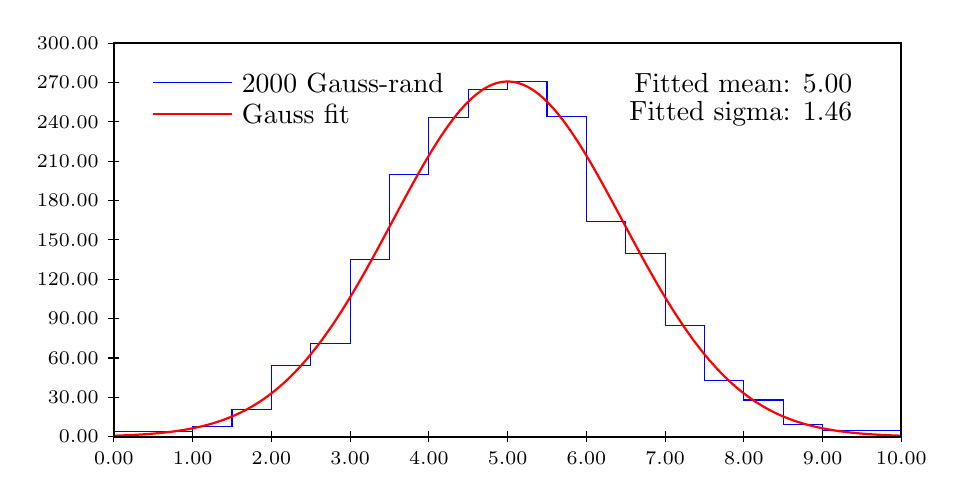
\begin{tikzpicture}[]
\begin{scope}[]
\clip (0.0,0.0) rectangle (10.0,5.0);
\begin{scope}[shift={(0.0,0.0)}]
\pgfsetxvec{\pgfpoint{1.0cm}{0cm}}
\pgfsetyvec{\pgfpoint{0cm}{0.016666668cm}}
\begin{scope}[shift={(0.0,0.0)}]
\begin{scope}[draw=blue]
\pgfpathmoveto{ \pgfpointxy {10.0} {0.0}}
\pgfpathlineto{ \pgfpointxy {10.0} {5.0}}
\pgfpathlineto{ \pgfpointxy {9.5} {5.0}}
\pgfpathlineto{ \pgfpointxy {9.5} {5.0}}
\pgfpathlineto{ \pgfpointxy {9.0} {5.0}}
\pgfpathlineto{ \pgfpointxy {9.0} {9.0}}
\pgfpathlineto{ \pgfpointxy {8.5} {9.0}}
\pgfpathlineto{ \pgfpointxy {8.5} {28.0}}
\pgfpathlineto{ \pgfpointxy {8.0} {28.0}}
\pgfpathlineto{ \pgfpointxy {8.0} {43.0}}
\pgfpathlineto{ \pgfpointxy {7.5} {43.0}}
\pgfpathlineto{ \pgfpointxy {7.5} {85.0}}
\pgfpathlineto{ \pgfpointxy {7.0} {85.0}}
\pgfpathlineto{ \pgfpointxy {7.0} {140.0}}
\pgfpathlineto{ \pgfpointxy {6.5} {140.0}}
\pgfpathlineto{ \pgfpointxy {6.5} {164.0}}
\pgfpathlineto{ \pgfpointxy {6.0} {164.0}}
\pgfpathlineto{ \pgfpointxy {6.0} {244.0}}
\pgfpathlineto{ \pgfpointxy {5.5} {244.0}}
\pgfpathlineto{ \pgfpointxy {5.5} {271.0}}
\pgfpathlineto{ \pgfpointxy {5.0} {271.0}}
\pgfpathlineto{ \pgfpointxy {5.0} {265.0}}
\pgfpathlineto{ \pgfpointxy {4.5} {265.0}}
\pgfpathlineto{ \pgfpointxy {4.5} {243.0}}
\pgfpathlineto{ \pgfpointxy {4.0} {243.0}}
\pgfpathlineto{ \pgfpointxy {4.0} {200.0}}
\pgfpathlineto{ \pgfpointxy {3.5} {200.0}}
\pgfpathlineto{ \pgfpointxy {3.5} {135.0}}
\pgfpathlineto{ \pgfpointxy {3.0} {135.0}}
\pgfpathlineto{ \pgfpointxy {3.0} {71.0}}
\pgfpathlineto{ \pgfpointxy {2.5} {71.0}}
\pgfpathlineto{ \pgfpointxy {2.5} {54.0}}
\pgfpathlineto{ \pgfpointxy {2.0} {54.0}}
\pgfpathlineto{ \pgfpointxy {2.0} {21.0}}
\pgfpathlineto{ \pgfpointxy {1.5} {21.0}}
\pgfpathlineto{ \pgfpointxy {1.5} {8.0}}
\pgfpathlineto{ \pgfpointxy {1.0} {8.0}}
\pgfpathlineto{ \pgfpointxy {1.0} {4.0}}
\pgfpathlineto{ \pgfpointxy {0.5} {4.0}}
\pgfpathlineto{ \pgfpointxy {0.5} {4.0}}
\pgfpathlineto{ \pgfpointxy {0.0} {4.0}}
\pgfpathlineto{ \pgfpointxy {0.0} {0.0}}
\pgfusepath{ stroke, }
\end{scope}
\end{scope}
\pgfsetxvec{\pgfpoint{1cm}{0cm}}
\pgfsetyvec{\pgfpoint{0cm}{1cm}}
\end{scope}
\end{scope}
\node[left] at (9.5,4.5) {Fitted mean:  5.00};
\node[left] at (9.5,4.1) {Fitted sigma:  1.46};
\begin{scope}[]
\clip (0.0,0.0) rectangle (10.0,5.0);
\begin{scope}[shift={(0.0,0.0)}]
\pgfsetxvec{\pgfpoint{1.0cm}{0cm}}
\pgfsetyvec{\pgfpoint{0cm}{0.016666668cm}}
\begin{scope}[shift={(0.0,0.0)}]
\begin{scope}[thick,red]
\pgfpathmoveto{ \pgfpointxy {0.0} {0.785533585190544}}
\pgfpathlineto{ \pgfpointxy {0.05} {0.8823944062104124}}
\pgfpathlineto{ \pgfpointxy {0.1} {0.9900410132316494}}
\pgfpathlineto{ \pgfpointxy {0.15} {1.1095224058046345}}
\pgfpathlineto{ \pgfpointxy {0.2} {1.2419708963422873}}
\pgfpathlineto{ \pgfpointxy {0.25} {1.3886065589283518}}
\pgfpathlineto{ \pgfpointxy {0.3} {1.5507416694118887}}
\pgfpathlineto{ \pgfpointxy {0.35} {1.7297851028337528}}
\pgfpathlineto{ \pgfpointxy {0.4} {1.927246650571349}}
\pgfpathlineto{ \pgfpointxy {0.45} {2.144741215868452}}
\pgfpathlineto{ \pgfpointxy {0.5} {2.383992842671168}}
\pgfpathlineto{ \pgfpointxy {0.55} {2.646838528957892}}
\pgfpathlineto{ \pgfpointxy {0.6} {2.935231772073318}}
\pgfpathlineto{ \pgfpointxy {0.65} {3.251245790000996}}
\pgfpathlineto{ \pgfpointxy {0.7} {3.5970763590868597}}
\pgfpathlineto{ \pgfpointxy {0.75} {3.9750442055123947}}
\pgfpathlineto{ \pgfpointxy {0.8} {4.387596884868998}}
\pgfpathlineto{ \pgfpointxy {0.85} {4.8373100815661525}}
\pgfpathlineto{ \pgfpointxy {0.9} {5.326888257579253}}
\pgfpathlineto{ \pgfpointxy {0.95} {5.859164578274084}}
\pgfpathlineto{ \pgfpointxy {1.0} {6.437100041802212}}
\pgfpathlineto{ \pgfpointxy {1.05} {7.063781737911131}}
\pgfpathlineto{ \pgfpointxy {1.1} {7.742420162024598}}
\pgfpathlineto{ \pgfpointxy {1.15} {8.476345511186555}}
\pgfpathlineto{ \pgfpointxy {1.2} {9.269002889991516}}
\pgfpathlineto{ \pgfpointxy {1.25} {10.12394635700542}}
\pgfpathlineto{ \pgfpointxy {1.3} {11.044831745470251}}
\pgfpathlineto{ \pgfpointxy {1.35} {12.035408196332893}}
\pgfpathlineto{ \pgfpointxy {1.4} {13.099508346888094}}
\pgfpathlineto{ \pgfpointxy {1.45} {14.241037124611898}}
\pgfpathlineto{ \pgfpointxy {1.5} {15.463959103111062}}
\pgfpathlineto{ \pgfpointxy {1.55} {16.77228438554224}}
\pgfpathlineto{ \pgfpointxy {1.6} {18.170052990364315}}
\pgfpathlineto{ \pgfpointxy {1.65} {19.661317724870088}}
\pgfpathlineto{ \pgfpointxy {1.7} {21.250125543575855}}
\pgfpathlineto{ \pgfpointxy {1.75} {22.940497401191028}}
\pgfpathlineto{ \pgfpointxy {1.8} {24.736406623493174}}
\pgfpathlineto{ \pgfpointxy {1.85} {26.64175583392414}}
\pgfpathlineto{ \pgfpointxy {1.9} {28.660352489018294}}
\pgfpathlineto{ \pgfpointxy {1.95} {30.795883091768726}}
\pgfpathlineto{ \pgfpointxy {2.0} {33.05188616861204}}
\pgfpathlineto{ \pgfpointxy {2.05} {35.431724112736475}}
\pgfpathlineto{ \pgfpointxy {2.1} {37.938554013731526}}
\pgfpathlineto{ \pgfpointxy {2.15} {40.57529761104231}}
\pgfpathlineto{ \pgfpointxy {2.2} {43.34461052608296}}
\pgfpathlineto{ \pgfpointxy {2.25} {46.248850945007725}}
\pgfpathlineto{ \pgfpointxy {2.3} {49.290047940835414}}
\pgfpathlineto{ \pgfpointxy {2.35} {52.46986963965609}}
\pgfpathlineto{ \pgfpointxy {2.4} {55.789591450800295}}
\pgfpathlineto{ \pgfpointxy {2.45} {59.25006459489787}}
\pgfpathlineto{ \pgfpointxy {2.5} {62.85168517646614}}
\pgfpathlineto{ \pgfpointxy {2.55} {66.5943640588275}}
\pgfpathlineto{ \pgfpointxy {2.6} {70.47749780853638}}
\pgfpathlineto{ \pgfpointxy {2.65} {74.49994098389061}}
\pgfpathlineto{ \pgfpointxy {2.7} {78.65998004730363}}
\pgfpathlineto{ \pgfpointxy {2.75} {82.9553091841374}}
\pgfpathlineto{ \pgfpointxy {2.8} {87.38300831087108}}
\pgfpathlineto{ \pgfpointxy {2.85} {91.93952355305386}}
\pgfpathlineto{ \pgfpointxy {2.9} {96.62065046824108}}
\pgfpathlineto{ \pgfpointxy {2.95} {101.42152028093761}}
\pgfpathlineto{ \pgfpointxy {3.0} {106.33658938540171}}
\pgfpathlineto{ \pgfpointxy {3.05} {111.35963235796345}}
\pgfpathlineto{ \pgfpointxy {3.1} {116.48373870327391}}
\pgfpathlineto{ \pgfpointxy {3.15} {121.70131353866445}}
\pgfpathlineto{ \pgfpointxy {3.2} {127.00408239762504}}
\pgfpathlineto{ \pgfpointxy {3.25} {132.38310030741803}}
\pgfpathlineto{ \pgfpointxy {3.3} {137.82876526717794}}
\pgfpathlineto{ \pgfpointxy {3.35} {143.3308362216892}}
\pgfpathlineto{ \pgfpointxy {3.4} {148.87845559261598}}
\pgfpathlineto{ \pgfpointxy {3.45} {154.4601763935346}}
\pgfpathlineto{ \pgfpointxy {3.5} {160.06399391798755}}
\pgfpathlineto{ \pgfpointxy {3.55} {165.67738195127163}}
\pgfpathlineto{ \pgfpointxy {3.6} {171.28733341714147}}
\pgfpathlineto{ \pgfpointxy {3.65} {176.88040533044696}}
\pgfpathlineto{ \pgfpointxy {3.7} {182.4427678863249}}
\pgfpathlineto{ \pgfpointxy {3.75} {187.96025747636367}}
\pgfpathlineto{ \pgfpointxy {3.8} {193.4184333825861}}
\pgfpathlineto{ \pgfpointxy {3.85} {198.8026378615926}}
\pgfpathlineto{ \pgfpointxy {3.9} {204.0980592942233}}
\pgfpathlineto{ \pgfpointxy {3.95} {209.2897980410712}}
\pgfpathlineto{ \pgfpointxy {4.0} {214.36293461154008}}
\pgfpathlineto{ \pgfpointxy {4.05} {219.30259972431023}}
\pgfpathlineto{ \pgfpointxy {4.1} {224.09404581043842}}
\pgfpathlineto{ \pgfpointxy {4.15} {228.7227194872519}}
\pgfpathlineto{ \pgfpointxy {4.2} {233.1743345120225}}
\pgfpathlineto{ \pgfpointxy {4.25} {237.43494470943358}}
\pgfpathlineto{ \pgfpointxy {4.3} {241.4910163563196}}
\pgfpathlineto{ \pgfpointxy {4.35} {245.32949950128543}}
\pgfpathlineto{ \pgfpointxy {4.4} {248.93789769574337}}
\pgfpathlineto{ \pgfpointxy {4.45} {252.30433561675085}}
\pgfpathlineto{ \pgfpointxy {4.5} {255.4176240708332}}
\pgfpathlineto{ \pgfpointxy {4.55} {258.26732188172053}}
\pgfpathlineto{ \pgfpointxy {4.6} {260.84379418355206}}
\pgfpathlineto{ \pgfpointxy {4.65} {263.13826666446903}}
\pgfpathlineto{ \pgfpointxy {4.7} {265.14287533345066}}
\pgfpathlineto{ \pgfpointxy {4.75} {266.8507114154981}}
\pgfpathlineto{ \pgfpointxy {4.8} {268.25586101655}}
\pgfpathlineto{ \pgfpointxy {4.85} {269.35343923947187}}
\pgfpathlineto{ \pgfpointxy {4.9} {270.1396184757107}}
\pgfpathlineto{ \pgfpointxy {4.95} {270.6116506433102}}
\pgfpathlineto{ \pgfpointxy {5.0} {270.76788319047864}}
\pgfpathlineto{ \pgfpointxy {5.05} {270.6077687342832}}
\pgfpathlineto{ \pgfpointxy {5.1} {270.1318682557956}}
\pgfpathlineto{ \pgfpointxy {5.15} {269.3418478255878}}
\pgfpathlineto{ \pgfpointxy {5.2} {268.24046888632785}}
\pgfpathlineto{ \pgfpointxy {5.25} {266.8315721717906}}
\pgfpathlineto{ \pgfpointxy {5.3} {265.1200553933392}}
\pgfpathlineto{ \pgfpointxy {5.35} {263.11184487529204}}
\pgfpathlineto{ \pgfpointxy {5.4} {260.81386136906104}}
\pgfpathlineto{ \pgfpointxy {5.45} {258.23398032201965}}
\pgfpathlineto{ \pgfpointxy {5.5} {255.38098692026887}}
\pgfpathlineto{ \pgfpointxy {5.55} {252.26452626438723}}
\pgfpathlineto{ \pgfpointxy {5.6} {248.89504907347904}}
\pgfpathlineto{ \pgfpointxy {5.65} {245.28375334503724}}
\pgfpathlineto{ \pgfpointxy {5.7} {241.44252242601453}}
\pgfpathlineto{ \pgfpointxy {5.75} {237.38385997380678}}
\pgfpathlineto{ \pgfpointxy {5.8} {233.12082230441845}}
\pgfpathlineto{ \pgfpointxy {5.85} {228.66694863876333}}
\pgfpathlineto{ \pgfpointxy {5.9} {224.03618976679525}}
\pgfpathlineto{ \pgfpointxy {5.95} {219.2428356529474}}
\pgfpathlineto{ \pgfpointxy {6.0} {214.3014425052294}}
\pgfpathlineto{ \pgfpointxy {6.05} {209.22675982440097}}
\pgfpathlineto{ \pgfpointxy {6.1} {204.03365793905297}}
\pgfpathlineto{ \pgfpointxy {6.15} {198.73705651739786}}
\pgfpathlineto{ \pgfpointxy {6.2} {193.35185452735166}}
\pgfpathlineto{ \pgfpointxy {6.25} {187.8928620933718}}
\pgfpathlineto{ \pgfpointxy {6.3} {182.3747346718441}}
\pgfpathlineto{ \pgfpointxy {6.35} {176.81190993693747}}
\pgfpathlineto{ \pgfpointxy {6.4} {171.21854773617946}}
\pgfpathlineto{ \pgfpointxy {6.45} {165.6084734399515}}
\pgfpathlineto{ \pgfpointxy {6.5} {159.99512497209525}}
\pgfpathlineto{ \pgfpointxy {6.55} {154.39150377030742}}
\pgfpathlineto{ \pgfpointxy {6.6} {148.81012988541192}}
\pgfpathlineto{ \pgfpointxy {6.65} {143.26300138839366}}
\pgfpathlineto{ \pgfpointxy {6.7} {137.76155821368138}}
\pgfpathlineto{ \pgfpointxy {6.75} {132.31665052700623}}
\pgfpathlineto{ \pgfpointxy {6.8} {126.93851166664665}}
\pgfpathlineto{ \pgfpointxy {6.85} {121.63673566837342}}
\pgfpathlineto{ \pgfpointxy {6.9} {116.4202593472993}}
\pgfpathlineto{ \pgfpointxy {6.95} {111.29734887443767}}
\pgfpathlineto{ \pgfpointxy {7.0} {106.27559075237848}}
\pgfpathlineto{ \pgfpointxy {7.05} {101.36188706336671}}
\pgfpathlineto{ \pgfpointxy {7.1} {96.56245483442952}}
\pgfpathlineto{ \pgfpointxy {7.15} {91.88282933824159}}
\pgfpathlineto{ \pgfpointxy {7.2} {87.32787112528398}}
\pgfpathlineto{ \pgfpointxy {7.25} {82.90177656264828}}
\pgfpathlineto{ \pgfpointxy {7.3} {78.60809163764216}}
\pgfpathlineto{ \pgfpointxy {7.35} {74.44972877018493}}
\pgfpathlineto{ \pgfpointxy {7.4} {70.4289863668524}}
\pgfpathlineto{ \pgfpointxy {7.45} {66.5475708412896}}
\pgfpathlineto{ \pgfpointxy {7.5} {62.80662082049553}}
\pgfpathlineto{ \pgfpointxy {7.55} {59.20673325409326}}
\pgfpathlineto{ \pgfpointxy {7.6} {55.74799114400455}}
\pgfpathlineto{ \pgfpointxy {7.65} {52.42999261480181}}
\pgfpathlineto{ \pgfpointxy {7.7} {49.25188105024186}}
\pgfpathlineto{ \pgfpointxy {7.75} {46.2123760289026}}
\pgfpathlineto{ \pgfpointxy {7.8} {43.30980480125177}}
\pgfpathlineto{ \pgfpointxy {7.85} {40.54213406165323}}
\pgfpathlineto{ \pgfpointxy {7.9} {37.90700178154938}}
\pgfpathlineto{ \pgfpointxy {7.95} {35.40174888411922}}
\pgfpathlineto{ \pgfpointxy {8.0} {33.02345055587413}}
\pgfpathlineto{ \pgfpointxy {8.05} {30.768947006698582}}
\pgfpathlineto{ \pgfpointxy {8.1} {28.6348735065443}}
\pgfpathlineto{ \pgfpointxy {8.15} {26.61768954413513}}
\pgfpathlineto{ \pgfpointxy {8.2} {24.713706970436572}}
\pgfpathlineto{ \pgfpointxy {8.25} {22.91911700708104}}
\pgfpathlineto{ \pgfpointxy {8.3} {21.230016017259846}}
\pgfpathlineto{ \pgfpointxy {8.35} {19.642429953603866}}
\pgfpathlineto{ \pgfpointxy {8.4} {18.152337414149354}}
\pgfpathlineto{ \pgfpointxy {8.45} {16.75569125346978}}
\pgfpathlineto{ \pgfpointxy {8.5} {15.448438711340048}}
\pgfpathlineto{ \pgfpointxy {8.55} {14.226540035781417}}
\pgfpathlineto{ \pgfpointxy {8.6} {13.08598559092523}}
\pgfpathlineto{ \pgfpointxy {8.65} {12.022811452766204}}
\pgfpathlineto{ \pgfpointxy {8.7} {11.033113507495788}}
\pgfpathlineto{ \pgfpointxy {8.75} {10.1130600776746}}
\pgfpathlineto{ \pgfpointxy {8.8} {9.258903111001242}}
\pgfpathlineto{ \pgfpointxy {8.85} {8.4669879748478}}
\pgfpathlineto{ \pgfpointxy {8.9} {7.733761907069523}}
\pgfpathlineto{ \pgfpointxy {8.95} {7.055781179870019}}
\pgfpathlineto{ \pgfpointxy {9.0} {6.429717038738498}}
\pgfpathlineto{ \pgfpointxy {9.05} {5.852360482713078}}
\pgfpathlineto{ \pgfpointxy {9.1} {5.320625955499768}}
\pgfpathlineto{ \pgfpointxy {9.15} {4.8315540193486735}}
\pgfpathlineto{ \pgfpointxy {9.2} {4.382313085107549}}
\pgfpathlineto{ \pgfpointxy {9.25} {3.9702002726017023}}
\pgfpathlineto{ \pgfpointxy {9.3} {3.5926414754922513}}
\pgfpathlineto{ \pgfpointxy {9.35} {3.2471907041067585}}
\pgfpathlineto{ \pgfpointxy {9.4} {2.931528778486455}}
\pgfpathlineto{ \pgfpointxy {9.45} {2.643461442119739}}
\pgfpathlineto{ \pgfpointxy {9.5} {2.380916964599145}}
\pgfpathlineto{ \pgfpointxy {9.55} {2.1419432988161606}}
\pgfpathlineto{ \pgfpointxy {9.6} {1.9247048553571429}}
\pgfpathlineto{ \pgfpointxy {9.65} {1.7274789535470048}}
\pgfpathlineto{ \pgfpointxy {9.7} {1.5486520051633315}}
\pgfpathlineto{ \pgfpointxy {9.75} {1.3867154832659307}}
\pgfpathlineto{ \pgfpointxy {9.8} {1.2402617249087116}}
\pgfpathlineto{ \pgfpointxy {9.85} {1.1079796127665273}}
\pgfpathlineto{ \pgfpointxy {9.9} {0.9886501769645344}}
\pgfpathlineto{ \pgfpointxy {9.95} {0.8811421546783109}}
\pgfpathlineto{ \pgfpointxy {10.0} {0.7844075414145795}}
\pgfusepath{ stroke, }
\end{scope}
\end{scope}
\pgfsetxvec{\pgfpoint{1cm}{0cm}}
\pgfsetyvec{\pgfpoint{0cm}{1cm}}
\end{scope}
\end{scope}
\begin{scope}[shift={(0.0,0.0)}]
\pgfsetxvec{\pgfpoint{1.0cm}{0cm}}
\pgfsetyvec{\pgfpoint{0cm}{0.016666668cm}}
\begin{scope}[shift={(0.0,0.0)}]
\begin{scope}[yshift=0cm]
\draw[black] [shift={(0.0,0.0)}] (0,2pt) -- (0,-2pt) node[below]{ \scriptsize{\num[round-mode=places,round-precision=2]{0}}};
\draw[black] [shift={(1.0,0.0)}] (0,2pt) -- (0,-2pt) node[below]{ \scriptsize{\num[round-mode=places,round-precision=2]{1}}};
\draw[black] [shift={(2.0,0.0)}] (0,2pt) -- (0,-2pt) node[below]{ \scriptsize{\num[round-mode=places,round-precision=2]{2}}};
\draw[black] [shift={(3.0,0.0)}] (0,2pt) -- (0,-2pt) node[below]{ \scriptsize{\num[round-mode=places,round-precision=2]{3}}};
\draw[black] [shift={(4.0,0.0)}] (0,2pt) -- (0,-2pt) node[below]{ \scriptsize{\num[round-mode=places,round-precision=2]{4}}};
\draw[black] [shift={(5.0,0.0)}] (0,2pt) -- (0,-2pt) node[below]{ \scriptsize{\num[round-mode=places,round-precision=2]{5}}};
\draw[black] [shift={(6.0,0.0)}] (0,2pt) -- (0,-2pt) node[below]{ \scriptsize{\num[round-mode=places,round-precision=2]{6}}};
\draw[black] [shift={(7.0,0.0)}] (0,2pt) -- (0,-2pt) node[below]{ \scriptsize{\num[round-mode=places,round-precision=2]{7}}};
\draw[black] [shift={(8.0,0.0)}] (0,2pt) -- (0,-2pt) node[below]{ \scriptsize{\num[round-mode=places,round-precision=2]{8}}};
\draw[black] [shift={(9.0,0.0)}] (0,2pt) -- (0,-2pt) node[below]{ \scriptsize{\num[round-mode=places,round-precision=2]{9}}};
\draw[black] [shift={(10.0,0.0)}] (0,2pt) -- (0,-2pt) node[below]{ \scriptsize{\num[round-mode=places,round-precision=2]{10}}};
\end{scope}
\begin{scope}[xshift=0cm]
\draw[black] [shift={(0.0,0.0)}] (2pt,0) -- (-2pt,0) node[left]{ \scriptsize{\num[round-mode=places,round-precision=2]{0}}};
\draw[black] [shift={(0.0,30.0)}] (2pt,0) -- (-2pt,0) node[left]{ \scriptsize{\num[round-mode=places,round-precision=2]{30}}};
\draw[black] [shift={(0.0,60.0)}] (2pt,0) -- (-2pt,0) node[left]{ \scriptsize{\num[round-mode=places,round-precision=2]{60}}};
\draw[black] [shift={(0.0,90.0)}] (2pt,0) -- (-2pt,0) node[left]{ \scriptsize{\num[round-mode=places,round-precision=2]{90}}};
\draw[black] [shift={(0.0,120.0)}] (2pt,0) -- (-2pt,0) node[left]{ \scriptsize{\num[round-mode=places,round-precision=2]{120}}};
\draw[black] [shift={(0.0,150.0)}] (2pt,0) -- (-2pt,0) node[left]{ \scriptsize{\num[round-mode=places,round-precision=2]{150}}};
\draw[black] [shift={(0.0,180.0)}] (2pt,0) -- (-2pt,0) node[left]{ \scriptsize{\num[round-mode=places,round-precision=2]{180}}};
\draw[black] [shift={(0.0,210.0)}] (2pt,0) -- (-2pt,0) node[left]{ \scriptsize{\num[round-mode=places,round-precision=2]{210}}};
\draw[black] [shift={(0.0,240.0)}] (2pt,0) -- (-2pt,0) node[left]{ \scriptsize{\num[round-mode=places,round-precision=2]{240}}};
\draw[black] [shift={(0.0,270.0)}] (2pt,0) -- (-2pt,0) node[left]{ \scriptsize{\num[round-mode=places,round-precision=2]{270}}};
\draw[black] [shift={(0.0,300.0)}] (2pt,0) -- (-2pt,0) node[left]{ \scriptsize{\num[round-mode=places,round-precision=2]{300}}};
\end{scope}
\end{scope}
\pgfsetxvec{\pgfpoint{1cm}{0cm}}
\pgfsetyvec{\pgfpoint{0cm}{1cm}}
\end{scope}
\draw[draw=blue,fill=blue] (0.5,4.5) -- (1.5,4.5);
\node[right,] at (1.5,4.5) {2000 Gauss-rand};
\draw[thick,red] (0.5,4.1) -- (1.5,4.1);
\node[right,] at (1.5,4.1) {Gauss fit};
\begin{scope}[thick,black,fill=white]
\pgfpathmoveto{ \pgfpointxy {0.0} {0.0}}
\pgfpathlineto{ \pgfpointxy {10.0} {0.0}}
\pgfpathlineto{ \pgfpointxy {10.0} {5.0}}
\pgfpathlineto{ \pgfpointxy {0.0} {5.0}}
\pgfpathclose
\pgfusepath{ stroke, }
\end{scope}
\end{tikzpicture}
%%% Local Variables: 
%%% mode: latex 
%%% TeX-master: "master" 
%%% End:


  \caption{The Gaussian function fitted to histogram made from 2000 gaussian random numbers}
\end{figure}

\begin{figure}[H]
  \centering
  %%% AUTO GENERATED CODE
\documentclass{standalone}
\ifx\HCode\UnDef\else\def\pgfsysdriver{pgfsys-tex4ht.def}\fi
\usepackage[usenames,dvipsnames,svgnames,table]{xcolor}
\usepackage{tikz}
\usepackage{color}
\usepackage{siunitx}
\usetikzlibrary{arrows,shapes}
\begin{document}
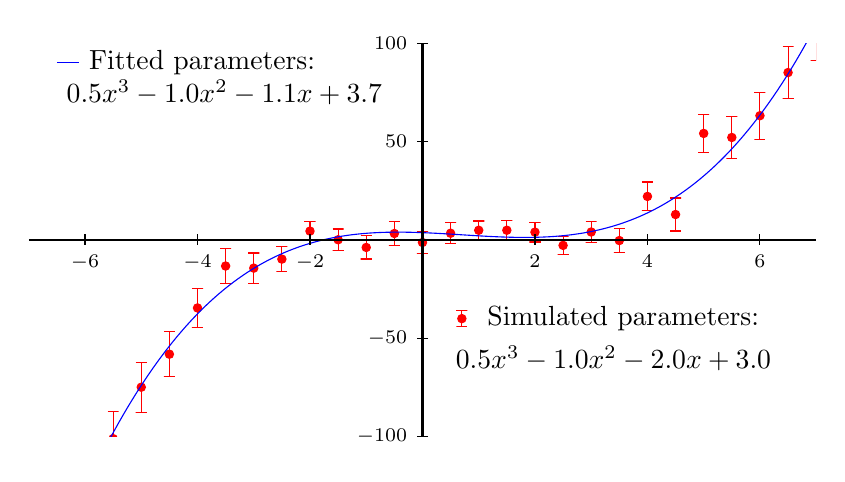
\begin{tikzpicture}
\begin{scope}[]
\pgfpathmoveto{ \pgfpointadd{\pgfpointxy {0.0} {0.0}} {\pgfpoint{0cm}{0cm}} }
\pgfpathlineto{ \pgfpointadd{\pgfpointxy {0.0} {0.0}} {\pgfpoint{10cm}{0cm}} }
\pgfpathlineto{ \pgfpointadd{\pgfpointxy {0.0} {0.0}} {\pgfpoint{10cm}{5cm}} }
\pgfpathlineto{ \pgfpointadd{\pgfpointxy {0.0} {0.0}} {\pgfpoint{0cm}{5cm}} }
\pgfpathclose
\pgfusepath{  clip, }
\begin{scope}[shift={(0.0,0.0)}]
\pgfsetxvec{\pgfpoint{0.71428573cm}{0cm}}
\pgfsetyvec{\pgfpoint{0cm}{0.025cm}}
\begin{scope}[shift={(7.0,100.0)}]
\begin{scope}[draw=red,fill=red]
\pgfpathmoveto{ \pgfpointadd{\pgfpointxy {-10.0} {-545.4404344594064}} {\pgfpoint{-2pt}{0}} }
\pgfpathlineto{ \pgfpointadd{\pgfpointxy {-10.0} {-545.4404344594064}} {\pgfpoint{2pt}{0}} }
\pgfpathlineto{ \pgfpointadd{\pgfpointxy {-10.0} {-545.4404344594064}} {\pgfpoint{0pt}{0}} }
\pgfpathlineto{ \pgfpointadd{\pgfpointxy {-10.0} {-601.4820830572636}} {\pgfpoint{0pt}{0}} }
\pgfpathlineto{ \pgfpointadd{\pgfpointxy {-10.0} {-601.4820830572636}} {\pgfpoint{-2pt}{0}} }
\pgfpathlineto{ \pgfpointadd{\pgfpointxy {-10.0} {-601.4820830572636}} {\pgfpoint{2pt}{0}} }
\pgfusepath{ stroke, }
\node at (-10.0,-573.461258758335) [draw=red,fill=red,circle,inner sep=0.0pt,minimum width =3.0pt,minimum height=3.0pt] {};
\end{scope}
\begin{scope}[draw=red,fill=red]
\pgfpathmoveto{ \pgfpointadd{\pgfpointxy {-9.5} {-447.18384020848845}} {\pgfpoint{-2pt}{0}} }
\pgfpathlineto{ \pgfpointadd{\pgfpointxy {-9.5} {-447.18384020848845}} {\pgfpoint{2pt}{0}} }
\pgfpathlineto{ \pgfpointadd{\pgfpointxy {-9.5} {-447.18384020848845}} {\pgfpoint{0pt}{0}} }
\pgfpathlineto{ \pgfpointadd{\pgfpointxy {-9.5} {-499.76803023141025}} {\pgfpoint{0pt}{0}} }
\pgfpathlineto{ \pgfpointadd{\pgfpointxy {-9.5} {-499.76803023141025}} {\pgfpoint{-2pt}{0}} }
\pgfpathlineto{ \pgfpointadd{\pgfpointxy {-9.5} {-499.76803023141025}} {\pgfpoint{2pt}{0}} }
\pgfusepath{ stroke, }
\node at (-9.5,-473.47593521994935) [draw=red,fill=red,circle,inner sep=0.0pt,minimum width =3.0pt,minimum height=3.0pt] {};
\end{scope}
\begin{scope}[draw=red,fill=red]
\pgfpathmoveto{ \pgfpointadd{\pgfpointxy {-9.0} {-393.55704978345085}} {\pgfpoint{-2pt}{0}} }
\pgfpathlineto{ \pgfpointadd{\pgfpointxy {-9.0} {-393.55704978345085}} {\pgfpoint{2pt}{0}} }
\pgfpathlineto{ \pgfpointadd{\pgfpointxy {-9.0} {-393.55704978345085}} {\pgfpoint{0pt}{0}} }
\pgfpathlineto{ \pgfpointadd{\pgfpointxy {-9.0} {-442.7638453395239}} {\pgfpoint{0pt}{0}} }
\pgfpathlineto{ \pgfpointadd{\pgfpointxy {-9.0} {-442.7638453395239}} {\pgfpoint{-2pt}{0}} }
\pgfpathlineto{ \pgfpointadd{\pgfpointxy {-9.0} {-442.7638453395239}} {\pgfpoint{2pt}{0}} }
\pgfusepath{ stroke, }
\node at (-9.0,-418.1604475614874) [draw=red,fill=red,circle,inner sep=0.0pt,minimum width =3.0pt,minimum height=3.0pt] {};
\end{scope}
\begin{scope}[draw=red,fill=red]
\pgfpathmoveto{ \pgfpointadd{\pgfpointxy {-8.5} {-308.27959989427444}} {\pgfpoint{-2pt}{0}} }
\pgfpathlineto{ \pgfpointadd{\pgfpointxy {-8.5} {-308.27959989427444}} {\pgfpoint{2pt}{0}} }
\pgfpathlineto{ \pgfpointadd{\pgfpointxy {-8.5} {-308.27959989427444}} {\pgfpoint{0pt}{0}} }
\pgfpathlineto{ \pgfpointadd{\pgfpointxy {-8.5} {-354.1906800688092}} {\pgfpoint{0pt}{0}} }
\pgfpathlineto{ \pgfpointadd{\pgfpointxy {-8.5} {-354.1906800688092}} {\pgfpoint{-2pt}{0}} }
\pgfpathlineto{ \pgfpointadd{\pgfpointxy {-8.5} {-354.1906800688092}} {\pgfpoint{2pt}{0}} }
\pgfusepath{ stroke, }
\node at (-8.5,-331.2351399815418) [draw=red,fill=red,circle,inner sep=0.0pt,minimum width =3.0pt,minimum height=3.0pt] {};
\end{scope}
\begin{scope}[draw=red,fill=red]
\pgfpathmoveto{ \pgfpointadd{\pgfpointxy {-8.0} {-239.37963398853427}} {\pgfpoint{-2pt}{0}} }
\pgfpathlineto{ \pgfpointadd{\pgfpointxy {-8.0} {-239.37963398853427}} {\pgfpoint{2pt}{0}} }
\pgfpathlineto{ \pgfpointadd{\pgfpointxy {-8.0} {-239.37963398853427}} {\pgfpoint{0pt}{0}} }
\pgfpathlineto{ \pgfpointadd{\pgfpointxy {-8.0} {-282.0783371343292}} {\pgfpoint{0pt}{0}} }
\pgfpathlineto{ \pgfpointadd{\pgfpointxy {-8.0} {-282.0783371343292}} {\pgfpoint{-2pt}{0}} }
\pgfpathlineto{ \pgfpointadd{\pgfpointxy {-8.0} {-282.0783371343292}} {\pgfpoint{2pt}{0}} }
\pgfusepath{ stroke, }
\node at (-8.0,-260.7289855614317) [draw=red,fill=red,circle,inner sep=0.0pt,minimum width =3.0pt,minimum height=3.0pt] {};
\end{scope}
\begin{scope}[draw=red,fill=red]
\pgfpathmoveto{ \pgfpointadd{\pgfpointxy {-7.5} {-197.49030193181449}} {\pgfpoint{-2pt}{0}} }
\pgfpathlineto{ \pgfpointadd{\pgfpointxy {-7.5} {-197.49030193181449}} {\pgfpoint{2pt}{0}} }
\pgfpathlineto{ \pgfpointadd{\pgfpointxy {-7.5} {-197.49030193181449}} {\pgfpoint{0pt}{0}} }
\pgfpathlineto{ \pgfpointadd{\pgfpointxy {-7.5} {-237.06164970158824}} {\pgfpoint{0pt}{0}} }
\pgfpathlineto{ \pgfpointadd{\pgfpointxy {-7.5} {-237.06164970158824}} {\pgfpoint{-2pt}{0}} }
\pgfpathlineto{ \pgfpointadd{\pgfpointxy {-7.5} {-237.06164970158824}} {\pgfpoint{2pt}{0}} }
\pgfusepath{ stroke, }
\node at (-7.5,-217.27597581670136) [draw=red,fill=red,circle,inner sep=0.0pt,minimum width =3.0pt,minimum height=3.0pt] {};
\end{scope}
\begin{scope}[draw=red,fill=red]
\pgfpathmoveto{ \pgfpointadd{\pgfpointxy {-7.0} {-205.56046021847214}} {\pgfpoint{-2pt}{0}} }
\pgfpathlineto{ \pgfpointadd{\pgfpointxy {-7.0} {-205.56046021847214}} {\pgfpoint{2pt}{0}} }
\pgfpathlineto{ \pgfpointadd{\pgfpointxy {-7.0} {-205.56046021847214}} {\pgfpoint{0pt}{0}} }
\pgfpathlineto{ \pgfpointadd{\pgfpointxy {-7.0} {-242.09114545384637}} {\pgfpoint{0pt}{0}} }
\pgfpathlineto{ \pgfpointadd{\pgfpointxy {-7.0} {-242.09114545384637}} {\pgfpoint{-2pt}{0}} }
\pgfpathlineto{ \pgfpointadd{\pgfpointxy {-7.0} {-242.09114545384637}} {\pgfpoint{2pt}{0}} }
\pgfusepath{ stroke, }
\node at (-7.0,-223.82580283615926) [draw=red,fill=red,circle,inner sep=0.0pt,minimum width =3.0pt,minimum height=3.0pt] {};
\end{scope}
\begin{scope}[draw=red,fill=red]
\pgfpathmoveto{ \pgfpointadd{\pgfpointxy {-6.5} {-139.84137726003047}} {\pgfpoint{-2pt}{0}} }
\pgfpathlineto{ \pgfpointadd{\pgfpointxy {-6.5} {-139.84137726003047}} {\pgfpoint{2pt}{0}} }
\pgfpathlineto{ \pgfpointadd{\pgfpointxy {-6.5} {-139.84137726003047}} {\pgfpoint{0pt}{0}} }
\pgfpathlineto{ \pgfpointadd{\pgfpointxy {-6.5} {-173.41968838488776}} {\pgfpoint{0pt}{0}} }
\pgfpathlineto{ \pgfpointadd{\pgfpointxy {-6.5} {-173.41968838488776}} {\pgfpoint{-2pt}{0}} }
\pgfpathlineto{ \pgfpointadd{\pgfpointxy {-6.5} {-173.41968838488776}} {\pgfpoint{2pt}{0}} }
\pgfusepath{ stroke, }
\node at (-6.5,-156.63053282245912) [draw=red,fill=red,circle,inner sep=0.0pt,minimum width =3.0pt,minimum height=3.0pt] {};
\end{scope}
\begin{scope}[draw=red,fill=red]
\pgfpathmoveto{ \pgfpointadd{\pgfpointxy {-6.0} {-137.03933110451544}} {\pgfpoint{-2pt}{0}} }
\pgfpathlineto{ \pgfpointadd{\pgfpointxy {-6.0} {-137.03933110451544}} {\pgfpoint{2pt}{0}} }
\pgfpathlineto{ \pgfpointadd{\pgfpointxy {-6.0} {-137.03933110451544}} {\pgfpoint{0pt}{0}} }
\pgfpathlineto{ \pgfpointadd{\pgfpointxy {-6.0} {-167.75496448771656}} {\pgfpoint{0pt}{0}} }
\pgfpathlineto{ \pgfpointadd{\pgfpointxy {-6.0} {-167.75496448771656}} {\pgfpoint{-2pt}{0}} }
\pgfpathlineto{ \pgfpointadd{\pgfpointxy {-6.0} {-167.75496448771656}} {\pgfpoint{2pt}{0}} }
\pgfusepath{ stroke, }
\node at (-6.0,-152.397147796116) [draw=red,fill=red,circle,inner sep=0.0pt,minimum width =3.0pt,minimum height=3.0pt] {};
\end{scope}
\begin{scope}[draw=red,fill=red]
\pgfpathmoveto{ \pgfpointadd{\pgfpointxy {-5.5} {-86.99694085231602}} {\pgfpoint{-2pt}{0}} }
\pgfpathlineto{ \pgfpointadd{\pgfpointxy {-5.5} {-86.99694085231602}} {\pgfpoint{2pt}{0}} }
\pgfpathlineto{ \pgfpointadd{\pgfpointxy {-5.5} {-86.99694085231602}} {\pgfpoint{0pt}{0}} }
\pgfpathlineto{ \pgfpointadd{\pgfpointxy {-5.5} {-114.94061152749515}} {\pgfpoint{0pt}{0}} }
\pgfpathlineto{ \pgfpointadd{\pgfpointxy {-5.5} {-114.94061152749515}} {\pgfpoint{-2pt}{0}} }
\pgfpathlineto{ \pgfpointadd{\pgfpointxy {-5.5} {-114.94061152749515}} {\pgfpoint{2pt}{0}} }
\pgfusepath{ stroke, }
\node at (-5.5,-100.96877618990558) [draw=red,fill=red,circle,inner sep=0.0pt,minimum width =3.0pt,minimum height=3.0pt] {};
\end{scope}
\begin{scope}[draw=red,fill=red]
\pgfpathmoveto{ \pgfpointadd{\pgfpointxy {-5.0} {-62.20168630127382}} {\pgfpoint{-2pt}{0}} }
\pgfpathlineto{ \pgfpointadd{\pgfpointxy {-5.0} {-62.20168630127382}} {\pgfpoint{2pt}{0}} }
\pgfpathlineto{ \pgfpointadd{\pgfpointxy {-5.0} {-62.20168630127382}} {\pgfpoint{0pt}{0}} }
\pgfpathlineto{ \pgfpointadd{\pgfpointxy {-5.0} {-87.46436280290588}} {\pgfpoint{0pt}{0}} }
\pgfpathlineto{ \pgfpointadd{\pgfpointxy {-5.0} {-87.46436280290588}} {\pgfpoint{-2pt}{0}} }
\pgfpathlineto{ \pgfpointadd{\pgfpointxy {-5.0} {-87.46436280290588}} {\pgfpoint{2pt}{0}} }
\pgfusepath{ stroke, }
\node at (-5.0,-74.83302455208985) [draw=red,fill=red,circle,inner sep=0.0pt,minimum width =3.0pt,minimum height=3.0pt] {};
\end{scope}
\begin{scope}[draw=red,fill=red]
\pgfpathmoveto{ \pgfpointadd{\pgfpointxy {-4.5} {-46.726130851753226}} {\pgfpoint{-2pt}{0}} }
\pgfpathlineto{ \pgfpointadd{\pgfpointxy {-4.5} {-46.726130851753226}} {\pgfpoint{2pt}{0}} }
\pgfpathlineto{ \pgfpointadd{\pgfpointxy {-4.5} {-46.726130851753226}} {\pgfpoint{0pt}{0}} }
\pgfpathlineto{ \pgfpointadd{\pgfpointxy {-4.5} {-69.39753160287444}} {\pgfpoint{0pt}{0}} }
\pgfpathlineto{ \pgfpointadd{\pgfpointxy {-4.5} {-69.39753160287444}} {\pgfpoint{-2pt}{0}} }
\pgfpathlineto{ \pgfpointadd{\pgfpointxy {-4.5} {-69.39753160287444}} {\pgfpoint{2pt}{0}} }
\pgfusepath{ stroke, }
\node at (-4.5,-58.06183122731383) [draw=red,fill=red,circle,inner sep=0.0pt,minimum width =3.0pt,minimum height=3.0pt] {};
\end{scope}
\begin{scope}[draw=red,fill=red]
\pgfpathmoveto{ \pgfpointadd{\pgfpointxy {-4.0} {-24.46841123687355}} {\pgfpoint{-2pt}{0}} }
\pgfpathlineto{ \pgfpointadd{\pgfpointxy {-4.0} {-24.46841123687355}} {\pgfpoint{2pt}{0}} }
\pgfpathlineto{ \pgfpointadd{\pgfpointxy {-4.0} {-24.46841123687355}} {\pgfpoint{0pt}{0}} }
\pgfpathlineto{ \pgfpointadd{\pgfpointxy {-4.0} {-44.63393629746999}} {\pgfpoint{0pt}{0}} }
\pgfpathlineto{ \pgfpointadd{\pgfpointxy {-4.0} {-44.63393629746999}} {\pgfpoint{-2pt}{0}} }
\pgfpathlineto{ \pgfpointadd{\pgfpointxy {-4.0} {-44.63393629746999}} {\pgfpoint{2pt}{0}} }
\pgfusepath{ stroke, }
\node at (-4.0,-34.55117376717177) [draw=red,fill=red,circle,inner sep=0.0pt,minimum width =3.0pt,minimum height=3.0pt] {};
\end{scope}
\begin{scope}[draw=red,fill=red]
\pgfpathmoveto{ \pgfpointadd{\pgfpointxy {-3.5} {-4.3839808804357165}} {\pgfpoint{-2pt}{0}} }
\pgfpathlineto{ \pgfpointadd{\pgfpointxy {-3.5} {-4.3839808804357165}} {\pgfpoint{2pt}{0}} }
\pgfpathlineto{ \pgfpointadd{\pgfpointxy {-3.5} {-4.3839808804357165}} {\pgfpoint{0pt}{0}} }
\pgfpathlineto{ \pgfpointadd{\pgfpointxy {-3.5} {-22.117942047401606}} {\pgfpoint{0pt}{0}} }
\pgfpathlineto{ \pgfpointadd{\pgfpointxy {-3.5} {-22.117942047401606}} {\pgfpoint{-2pt}{0}} }
\pgfpathlineto{ \pgfpointadd{\pgfpointxy {-3.5} {-22.117942047401606}} {\pgfpoint{2pt}{0}} }
\pgfusepath{ stroke, }
\node at (-3.5,-13.250961463918662) [draw=red,fill=red,circle,inner sep=0.0pt,minimum width =3.0pt,minimum height=3.0pt] {};
\end{scope}
\begin{scope}[draw=red,fill=red]
\pgfpathmoveto{ \pgfpointadd{\pgfpointxy {-3.0} {-6.647445276239654}} {\pgfpoint{-2pt}{0}} }
\pgfpathlineto{ \pgfpointadd{\pgfpointxy {-3.0} {-6.647445276239654}} {\pgfpoint{2pt}{0}} }
\pgfpathlineto{ \pgfpointadd{\pgfpointxy {-3.0} {-6.647445276239654}} {\pgfpoint{0pt}{0}} }
\pgfpathlineto{ \pgfpointadd{\pgfpointxy {-3.0} {-21.995914504589187}} {\pgfpoint{0pt}{0}} }
\pgfpathlineto{ \pgfpointadd{\pgfpointxy {-3.0} {-21.995914504589187}} {\pgfpoint{-2pt}{0}} }
\pgfpathlineto{ \pgfpointadd{\pgfpointxy {-3.0} {-21.995914504589187}} {\pgfpoint{2pt}{0}} }
\pgfusepath{ stroke, }
\node at (-3.0,-14.321679890414421) [draw=red,fill=red,circle,inner sep=0.0pt,minimum width =3.0pt,minimum height=3.0pt] {};
\end{scope}
\begin{scope}[draw=red,fill=red]
\pgfpathmoveto{ \pgfpointadd{\pgfpointxy {-2.5} {-3.2769548489061266}} {\pgfpoint{-2pt}{0}} }
\pgfpathlineto{ \pgfpointadd{\pgfpointxy {-2.5} {-3.2769548489061266}} {\pgfpoint{2pt}{0}} }
\pgfpathlineto{ \pgfpointadd{\pgfpointxy {-2.5} {-3.2769548489061266}} {\pgfpoint{0pt}{0}} }
\pgfpathlineto{ \pgfpointadd{\pgfpointxy {-2.5} {-16.20138374980418}} {\pgfpoint{0pt}{0}} }
\pgfpathlineto{ \pgfpointadd{\pgfpointxy {-2.5} {-16.20138374980418}} {\pgfpoint{-2pt}{0}} }
\pgfpathlineto{ \pgfpointadd{\pgfpointxy {-2.5} {-16.20138374980418}} {\pgfpoint{2pt}{0}} }
\pgfusepath{ stroke, }
\node at (-2.5,-9.739169299355153) [draw=red,fill=red,circle,inner sep=0.0pt,minimum width =3.0pt,minimum height=3.0pt] {};
\end{scope}
\begin{scope}[draw=red,fill=red]
\pgfpathmoveto{ \pgfpointadd{\pgfpointxy {-2.0} {9.4928432370132}} {\pgfpoint{-2pt}{0}} }
\pgfpathlineto{ \pgfpointadd{\pgfpointxy {-2.0} {9.4928432370132}} {\pgfpoint{2pt}{0}} }
\pgfpathlineto{ \pgfpointadd{\pgfpointxy {-2.0} {9.4928432370132}} {\pgfpoint{0pt}{0}} }
\pgfpathlineto{ \pgfpointadd{\pgfpointxy {-2.0} {-0.5071567629867992}} {\pgfpoint{0pt}{0}} }
\pgfpathlineto{ \pgfpointadd{\pgfpointxy {-2.0} {-0.5071567629867992}} {\pgfpoint{-2pt}{0}} }
\pgfpathlineto{ \pgfpointadd{\pgfpointxy {-2.0} {-0.5071567629867992}} {\pgfpoint{2pt}{0}} }
\pgfusepath{ stroke, }
\node at (-2.0,4.492843237013201) [draw=red,fill=red,circle,inner sep=0.0pt,minimum width =3.0pt,minimum height=3.0pt] {};
\end{scope}
\begin{scope}[draw=red,fill=red]
\pgfpathmoveto{ \pgfpointadd{\pgfpointxy {-1.5} {5.5385561325248664}} {\pgfpoint{-2pt}{0}} }
\pgfpathlineto{ \pgfpointadd{\pgfpointxy {-1.5} {5.5385561325248664}} {\pgfpoint{2pt}{0}} }
\pgfpathlineto{ \pgfpointadd{\pgfpointxy {-1.5} {5.5385561325248664}} {\pgfpoint{0pt}{0}} }
\pgfpathlineto{ \pgfpointadd{\pgfpointxy {-1.5} {-5.333725190744148}} {\pgfpoint{0pt}{0}} }
\pgfpathlineto{ \pgfpointadd{\pgfpointxy {-1.5} {-5.333725190744148}} {\pgfpoint{-2pt}{0}} }
\pgfpathlineto{ \pgfpointadd{\pgfpointxy {-1.5} {-5.333725190744148}} {\pgfpoint{2pt}{0}} }
\pgfusepath{ stroke, }
\node at (-1.5,0.10241547089035907) [draw=red,fill=red,circle,inner sep=0.0pt,minimum width =3.0pt,minimum height=3.0pt] {};
\end{scope}
\begin{scope}[draw=red,fill=red]
\pgfpathmoveto{ \pgfpointadd{\pgfpointxy {-1.0} {2.0474943682430817}} {\pgfpoint{-2pt}{0}} }
\pgfpathlineto{ \pgfpointadd{\pgfpointxy {-1.0} {2.0474943682430817}} {\pgfpoint{2pt}{0}} }
\pgfpathlineto{ \pgfpointadd{\pgfpointxy {-1.0} {2.0474943682430817}} {\pgfpoint{0pt}{0}} }
\pgfpathlineto{ \pgfpointadd{\pgfpointxy {-1.0} {-9.694163018530858}} {\pgfpoint{0pt}{0}} }
\pgfpathlineto{ \pgfpointadd{\pgfpointxy {-1.0} {-9.694163018530858}} {\pgfpoint{-2pt}{0}} }
\pgfpathlineto{ \pgfpointadd{\pgfpointxy {-1.0} {-9.694163018530858}} {\pgfpoint{2pt}{0}} }
\pgfusepath{ stroke, }
\node at (-1.0,-3.8233343251438887) [draw=red,fill=red,circle,inner sep=0.0pt,minimum width =3.0pt,minimum height=3.0pt] {};
\end{scope}
\begin{scope}[draw=red,fill=red]
\pgfpathmoveto{ \pgfpointadd{\pgfpointxy {-0.5} {9.199319361891407}} {\pgfpoint{-2pt}{0}} }
\pgfpathlineto{ \pgfpointadd{\pgfpointxy {-0.5} {9.199319361891407}} {\pgfpoint{2pt}{0}} }
\pgfpathlineto{ \pgfpointadd{\pgfpointxy {-0.5} {9.199319361891407}} {\pgfpoint{0pt}{0}} }
\pgfpathlineto{ \pgfpointadd{\pgfpointxy {-0.5} {-2.6412535120428977}} {\pgfpoint{0pt}{0}} }
\pgfpathlineto{ \pgfpointadd{\pgfpointxy {-0.5} {-2.6412535120428977}} {\pgfpoint{-2pt}{0}} }
\pgfpathlineto{ \pgfpointadd{\pgfpointxy {-0.5} {-2.6412535120428977}} {\pgfpoint{2pt}{0}} }
\pgfusepath{ stroke, }
\node at (-0.5,3.2790329249242545) [draw=red,fill=red,circle,inner sep=0.0pt,minimum width =3.0pt,minimum height=3.0pt] {};
\end{scope}
\begin{scope}[draw=red,fill=red]
\pgfpathmoveto{ \pgfpointadd{\pgfpointxy {0.0} {4.442405535239562}} {\pgfpoint{-2pt}{0}} }
\pgfpathlineto{ \pgfpointadd{\pgfpointxy {0.0} {4.442405535239562}} {\pgfpoint{2pt}{0}} }
\pgfpathlineto{ \pgfpointadd{\pgfpointxy {0.0} {4.442405535239562}} {\pgfpoint{0pt}{0}} }
\pgfpathlineto{ \pgfpointadd{\pgfpointxy {0.0} {-7.021696079898192}} {\pgfpoint{0pt}{0}} }
\pgfpathlineto{ \pgfpointadd{\pgfpointxy {0.0} {-7.021696079898192}} {\pgfpoint{-2pt}{0}} }
\pgfpathlineto{ \pgfpointadd{\pgfpointxy {0.0} {-7.021696079898192}} {\pgfpoint{2pt}{0}} }
\pgfusepath{ stroke, }
\node at (0.0,-1.2896452723293148) [draw=red,fill=red,circle,inner sep=0.0pt,minimum width =3.0pt,minimum height=3.0pt] {};
\end{scope}
\begin{scope}[draw=red,fill=red]
\pgfpathmoveto{ \pgfpointadd{\pgfpointxy {0.5} {8.757501632045631}} {\pgfpoint{-2pt}{0}} }
\pgfpathlineto{ \pgfpointadd{\pgfpointxy {0.5} {8.757501632045631}} {\pgfpoint{2pt}{0}} }
\pgfpathlineto{ \pgfpointadd{\pgfpointxy {0.5} {8.757501632045631}} {\pgfpoint{0pt}{0}} }
\pgfpathlineto{ \pgfpointadd{\pgfpointxy {0.5} {-1.93508077152162}} {\pgfpoint{0pt}{0}} }
\pgfpathlineto{ \pgfpointadd{\pgfpointxy {0.5} {-1.93508077152162}} {\pgfpoint{-2pt}{0}} }
\pgfpathlineto{ \pgfpointadd{\pgfpointxy {0.5} {-1.93508077152162}} {\pgfpoint{2pt}{0}} }
\pgfusepath{ stroke, }
\node at (0.5,3.411210430262006) [draw=red,fill=red,circle,inner sep=0.0pt,minimum width =3.0pt,minimum height=3.0pt] {};
\end{scope}
\begin{scope}[draw=red,fill=red]
\pgfpathmoveto{ \pgfpointadd{\pgfpointxy {1.0} {9.619207276103703}} {\pgfpoint{-2pt}{0}} }
\pgfpathlineto{ \pgfpointadd{\pgfpointxy {1.0} {9.619207276103703}} {\pgfpoint{2pt}{0}} }
\pgfpathlineto{ \pgfpointadd{\pgfpointxy {1.0} {9.619207276103703}} {\pgfpoint{0pt}{0}} }
\pgfpathlineto{ \pgfpointadd{\pgfpointxy {1.0} {0.20499371373060704}} {\pgfpoint{0pt}{0}} }
\pgfpathlineto{ \pgfpointadd{\pgfpointxy {1.0} {0.20499371373060704}} {\pgfpoint{-2pt}{0}} }
\pgfpathlineto{ \pgfpointadd{\pgfpointxy {1.0} {0.20499371373060704}} {\pgfpoint{2pt}{0}} }
\pgfusepath{ stroke, }
\node at (1.0,4.912100494917155) [draw=red,fill=red,circle,inner sep=0.0pt,minimum width =3.0pt,minimum height=3.0pt] {};
\end{scope}
\begin{scope}[draw=red,fill=red]
\pgfpathmoveto{ \pgfpointadd{\pgfpointxy {1.5} {9.676990570717388}} {\pgfpoint{-2pt}{0}} }
\pgfpathlineto{ \pgfpointadd{\pgfpointxy {1.5} {9.676990570717388}} {\pgfpoint{2pt}{0}} }
\pgfpathlineto{ \pgfpointadd{\pgfpointxy {1.5} {9.676990570717388}} {\pgfpoint{0pt}{0}} }
\pgfpathlineto{ \pgfpointadd{\pgfpointxy {1.5} {0.176990570717388}} {\pgfpoint{0pt}{0}} }
\pgfpathlineto{ \pgfpointadd{\pgfpointxy {1.5} {0.176990570717388}} {\pgfpoint{-2pt}{0}} }
\pgfpathlineto{ \pgfpointadd{\pgfpointxy {1.5} {0.176990570717388}} {\pgfpoint{2pt}{0}} }
\pgfusepath{ stroke, }
\node at (1.5,4.926990570717388) [draw=red,fill=red,circle,inner sep=0.0pt,minimum width =3.0pt,minimum height=3.0pt] {};
\end{scope}
\begin{scope}[draw=red,fill=red]
\pgfpathmoveto{ \pgfpointadd{\pgfpointxy {2.0} {8.978212194906977}} {\pgfpoint{-2pt}{0}} }
\pgfpathlineto{ \pgfpointadd{\pgfpointxy {2.0} {8.978212194906977}} {\pgfpoint{2pt}{0}} }
\pgfpathlineto{ \pgfpointadd{\pgfpointxy {2.0} {8.978212194906977}} {\pgfpoint{0pt}{0}} }
\pgfpathlineto{ \pgfpointadd{\pgfpointxy {2.0} {-1.0217878050930222}} {\pgfpoint{0pt}{0}} }
\pgfpathlineto{ \pgfpointadd{\pgfpointxy {2.0} {-1.0217878050930222}} {\pgfpoint{-2pt}{0}} }
\pgfpathlineto{ \pgfpointadd{\pgfpointxy {2.0} {-1.0217878050930222}} {\pgfpoint{2pt}{0}} }
\pgfusepath{ stroke, }
\node at (2.0,3.9782121949069778) [draw=red,fill=red,circle,inner sep=0.0pt,minimum width =3.0pt,minimum height=3.0pt] {};
\end{scope}
\begin{scope}[draw=red,fill=red]
\pgfpathmoveto{ \pgfpointadd{\pgfpointxy {2.5} {1.8969141840287458}} {\pgfpoint{-2pt}{0}} }
\pgfpathlineto{ \pgfpointadd{\pgfpointxy {2.5} {1.8969141840287458}} {\pgfpoint{2pt}{0}} }
\pgfpathlineto{ \pgfpointadd{\pgfpointxy {2.5} {1.8969141840287458}} {\pgfpoint{0pt}{0}} }
\pgfpathlineto{ \pgfpointadd{\pgfpointxy {2.5} {-7.425961471503549}} {\pgfpoint{0pt}{0}} }
\pgfpathlineto{ \pgfpointadd{\pgfpointxy {2.5} {-7.425961471503549}} {\pgfpoint{-2pt}{0}} }
\pgfpathlineto{ \pgfpointadd{\pgfpointxy {2.5} {-7.425961471503549}} {\pgfpoint{2pt}{0}} }
\pgfusepath{ stroke, }
\node at (2.5,-2.7645236437374017) [draw=red,fill=red,circle,inner sep=0.0pt,minimum width =3.0pt,minimum height=3.0pt] {};
\end{scope}
\begin{scope}[draw=red,fill=red]
\pgfpathmoveto{ \pgfpointadd{\pgfpointxy {3.0} {9.255509543307898}} {\pgfpoint{-2pt}{0}} }
\pgfpathlineto{ \pgfpointadd{\pgfpointxy {3.0} {9.255509543307898}} {\pgfpoint{2pt}{0}} }
\pgfpathlineto{ \pgfpointadd{\pgfpointxy {3.0} {9.255509543307898}} {\pgfpoint{0pt}{0}} }
\pgfpathlineto{ \pgfpointadd{\pgfpointxy {3.0} {-1.1939801994752797}} {\pgfpoint{0pt}{0}} }
\pgfpathlineto{ \pgfpointadd{\pgfpointxy {3.0} {-1.1939801994752797}} {\pgfpoint{-2pt}{0}} }
\pgfpathlineto{ \pgfpointadd{\pgfpointxy {3.0} {-1.1939801994752797}} {\pgfpoint{2pt}{0}} }
\pgfusepath{ stroke, }
\node at (3.0,4.03076467191631) [draw=red,fill=red,circle,inner sep=0.0pt,minimum width =3.0pt,minimum height=3.0pt] {};
\end{scope}
\begin{scope}[draw=red,fill=red]
\pgfpathmoveto{ \pgfpointadd{\pgfpointxy {3.5} {5.964258662648645}} {\pgfpoint{-2pt}{0}} }
\pgfpathlineto{ \pgfpointadd{\pgfpointxy {3.5} {5.964258662648645}} {\pgfpoint{2pt}{0}} }
\pgfpathlineto{ \pgfpointadd{\pgfpointxy {3.5} {5.964258662648645}} {\pgfpoint{0pt}{0}} }
\pgfpathlineto{ \pgfpointadd{\pgfpointxy {3.5} {-6.590958126923504}} {\pgfpoint{0pt}{0}} }
\pgfpathlineto{ \pgfpointadd{\pgfpointxy {3.5} {-6.590958126923504}} {\pgfpoint{-2pt}{0}} }
\pgfpathlineto{ \pgfpointadd{\pgfpointxy {3.5} {-6.590958126923504}} {\pgfpoint{2pt}{0}} }
\pgfusepath{ stroke, }
\node at (3.5,-0.31334973213742945) [draw=red,fill=red,circle,inner sep=0.0pt,minimum width =3.0pt,minimum height=3.0pt] {};
\end{scope}
\begin{scope}[draw=red,fill=red]
\pgfpathmoveto{ \pgfpointadd{\pgfpointxy {4.0} {29.421398911157304}} {\pgfpoint{-2pt}{0}} }
\pgfpathlineto{ \pgfpointadd{\pgfpointxy {4.0} {29.421398911157304}} {\pgfpoint{2pt}{0}} }
\pgfpathlineto{ \pgfpointadd{\pgfpointxy {4.0} {29.421398911157304}} {\pgfpoint{0pt}{0}} }
\pgfpathlineto{ \pgfpointadd{\pgfpointxy {4.0} {14.788149330446506}} {\pgfpoint{0pt}{0}} }
\pgfpathlineto{ \pgfpointadd{\pgfpointxy {4.0} {14.788149330446506}} {\pgfpoint{-2pt}{0}} }
\pgfpathlineto{ \pgfpointadd{\pgfpointxy {4.0} {14.788149330446506}} {\pgfpoint{2pt}{0}} }
\pgfusepath{ stroke, }
\node at (4.0,22.104774120801906) [draw=red,fill=red,circle,inner sep=0.0pt,minimum width =3.0pt,minimum height=3.0pt] {};
\end{scope}
\begin{scope}[draw=red,fill=red]
\pgfpathmoveto{ \pgfpointadd{\pgfpointxy {4.5} {21.306695411062467}} {\pgfpoint{-2pt}{0}} }
\pgfpathlineto{ \pgfpointadd{\pgfpointxy {4.5} {21.306695411062467}} {\pgfpoint{2pt}{0}} }
\pgfpathlineto{ \pgfpointadd{\pgfpointxy {4.5} {21.306695411062467}} {\pgfpoint{0pt}{0}} }
\pgfpathlineto{ \pgfpointadd{\pgfpointxy {4.5} {4.517497495438992}} {\pgfpoint{0pt}{0}} }
\pgfpathlineto{ \pgfpointadd{\pgfpointxy {4.5} {4.517497495438992}} {\pgfpoint{-2pt}{0}} }
\pgfpathlineto{ \pgfpointadd{\pgfpointxy {4.5} {4.517497495438992}} {\pgfpoint{2pt}{0}} }
\pgfusepath{ stroke, }
\node at (4.5,12.91209645325073) [draw=red,fill=red,circle,inner sep=0.0pt,minimum width =3.0pt,minimum height=3.0pt] {};
\end{scope}
\begin{scope}[draw=red,fill=red]
\pgfpathmoveto{ \pgfpointadd{\pgfpointxy {5.0} {63.64740104424042}} {\pgfpoint{-2pt}{0}} }
\pgfpathlineto{ \pgfpointadd{\pgfpointxy {5.0} {63.64740104424042}} {\pgfpoint{2pt}{0}} }
\pgfpathlineto{ \pgfpointadd{\pgfpointxy {5.0} {63.64740104424042}} {\pgfpoint{0pt}{0}} }
\pgfpathlineto{ \pgfpointadd{\pgfpointxy {5.0} {44.60204002705316}} {\pgfpoint{0pt}{0}} }
\pgfpathlineto{ \pgfpointadd{\pgfpointxy {5.0} {44.60204002705316}} {\pgfpoint{-2pt}{0}} }
\pgfpathlineto{ \pgfpointadd{\pgfpointxy {5.0} {44.60204002705316}} {\pgfpoint{2pt}{0}} }
\pgfusepath{ stroke, }
\node at (5.0,54.12472053564679) [draw=red,fill=red,circle,inner sep=0.0pt,minimum width =3.0pt,minimum height=3.0pt] {};
\end{scope}
\begin{scope}[draw=red,fill=red]
\pgfpathmoveto{ \pgfpointadd{\pgfpointxy {5.5} {62.77248248245576}} {\pgfpoint{-2pt}{0}} }
\pgfpathlineto{ \pgfpointadd{\pgfpointxy {5.5} {62.77248248245576}} {\pgfpoint{2pt}{0}} }
\pgfpathlineto{ \pgfpointadd{\pgfpointxy {5.5} {62.77248248245576}} {\pgfpoint{0pt}{0}} }
\pgfpathlineto{ \pgfpointadd{\pgfpointxy {5.5} {41.365394804663836}} {\pgfpoint{0pt}{0}} }
\pgfpathlineto{ \pgfpointadd{\pgfpointxy {5.5} {41.365394804663836}} {\pgfpoint{-2pt}{0}} }
\pgfpathlineto{ \pgfpointadd{\pgfpointxy {5.5} {41.365394804663836}} {\pgfpoint{2pt}{0}} }
\pgfusepath{ stroke, }
\node at (5.5,52.0689386435598) [draw=red,fill=red,circle,inner sep=0.0pt,minimum width =3.0pt,minimum height=3.0pt] {};
\end{scope}
\begin{scope}[draw=red,fill=red]
\pgfpathmoveto{ \pgfpointadd{\pgfpointxy {6.0} {75.06961524037354}} {\pgfpoint{-2pt}{0}} }
\pgfpathlineto{ \pgfpointadd{\pgfpointxy {6.0} {75.06961524037354}} {\pgfpoint{2pt}{0}} }
\pgfpathlineto{ \pgfpointadd{\pgfpointxy {6.0} {75.06961524037354}} {\pgfpoint{0pt}{0}} }
\pgfpathlineto{ \pgfpointadd{\pgfpointxy {6.0} {51.195107373985984}} {\pgfpoint{0pt}{0}} }
\pgfpathlineto{ \pgfpointadd{\pgfpointxy {6.0} {51.195107373985984}} {\pgfpoint{-2pt}{0}} }
\pgfpathlineto{ \pgfpointadd{\pgfpointxy {6.0} {51.195107373985984}} {\pgfpoint{2pt}{0}} }
\pgfusepath{ stroke, }
\node at (6.0,63.13236130717976) [draw=red,fill=red,circle,inner sep=0.0pt,minimum width =3.0pt,minimum height=3.0pt] {};
\end{scope}
\begin{scope}[draw=red,fill=red]
\pgfpathmoveto{ \pgfpointadd{\pgfpointxy {6.5} {98.27282162103023}} {\pgfpoint{-2pt}{0}} }
\pgfpathlineto{ \pgfpointadd{\pgfpointxy {6.5} {98.27282162103023}} {\pgfpoint{2pt}{0}} }
\pgfpathlineto{ \pgfpointadd{\pgfpointxy {6.5} {98.27282162103023}} {\pgfpoint{0pt}{0}} }
\pgfpathlineto{ \pgfpointadd{\pgfpointxy {6.5} {71.82695487533351}} {\pgfpoint{0pt}{0}} }
\pgfpathlineto{ \pgfpointadd{\pgfpointxy {6.5} {71.82695487533351}} {\pgfpoint{-2pt}{0}} }
\pgfpathlineto{ \pgfpointadd{\pgfpointxy {6.5} {71.82695487533351}} {\pgfpoint{2pt}{0}} }
\pgfusepath{ stroke, }
\node at (6.5,85.04988824818187) [draw=red,fill=red,circle,inner sep=0.0pt,minimum width =3.0pt,minimum height=3.0pt] {};
\end{scope}
\begin{scope}[draw=red,fill=red]
\pgfpathmoveto{ \pgfpointadd{\pgfpointxy {7.0} {120.17309324555772}} {\pgfpoint{-2pt}{0}} }
\pgfpathlineto{ \pgfpointadd{\pgfpointxy {7.0} {120.17309324555772}} {\pgfpoint{2pt}{0}} }
\pgfpathlineto{ \pgfpointadd{\pgfpointxy {7.0} {120.17309324555772}} {\pgfpoint{0pt}{0}} }
\pgfpathlineto{ \pgfpointadd{\pgfpointxy {7.0} {91.05438116361485}} {\pgfpoint{0pt}{0}} }
\pgfpathlineto{ \pgfpointadd{\pgfpointxy {7.0} {91.05438116361485}} {\pgfpoint{-2pt}{0}} }
\pgfpathlineto{ \pgfpointadd{\pgfpointxy {7.0} {91.05438116361485}} {\pgfpoint{2pt}{0}} }
\pgfusepath{ stroke, }
\node at (7.0,105.61373720458629) [draw=red,fill=red,circle,inner sep=0.0pt,minimum width =3.0pt,minimum height=3.0pt] {};
\end{scope}
\begin{scope}[draw=red,fill=red]
\pgfpathmoveto{ \pgfpointadd{\pgfpointxy {7.5} {151.1696495331387}} {\pgfpoint{-2pt}{0}} }
\pgfpathlineto{ \pgfpointadd{\pgfpointxy {7.5} {151.1696495331387}} {\pgfpoint{2pt}{0}} }
\pgfpathlineto{ \pgfpointadd{\pgfpointxy {7.5} {151.1696495331387}} {\pgfpoint{0pt}{0}} }
\pgfpathlineto{ \pgfpointadd{\pgfpointxy {7.5} {119.27927490233813}} {\pgfpoint{0pt}{0}} }
\pgfpathlineto{ \pgfpointadd{\pgfpointxy {7.5} {119.27927490233813}} {\pgfpoint{-2pt}{0}} }
\pgfpathlineto{ \pgfpointadd{\pgfpointxy {7.5} {119.27927490233813}} {\pgfpoint{2pt}{0}} }
\pgfusepath{ stroke, }
\node at (7.5,135.22446221773842) [draw=red,fill=red,circle,inner sep=0.0pt,minimum width =3.0pt,minimum height=3.0pt] {};
\end{scope}
\begin{scope}[draw=red,fill=red]
\pgfpathmoveto{ \pgfpointadd{\pgfpointxy {8.0} {174.93586539469865}} {\pgfpoint{-2pt}{0}} }
\pgfpathlineto{ \pgfpointadd{\pgfpointxy {8.0} {174.93586539469865}} {\pgfpoint{2pt}{0}} }
\pgfpathlineto{ \pgfpointadd{\pgfpointxy {8.0} {174.93586539469865}} {\pgfpoint{0pt}{0}} }
\pgfpathlineto{ \pgfpointadd{\pgfpointxy {8.0} {140.17768907417937}} {\pgfpoint{0pt}{0}} }
\pgfpathlineto{ \pgfpointadd{\pgfpointxy {8.0} {140.17768907417937}} {\pgfpoint{-2pt}{0}} }
\pgfpathlineto{ \pgfpointadd{\pgfpointxy {8.0} {140.17768907417937}} {\pgfpoint{2pt}{0}} }
\pgfusepath{ stroke, }
\node at (8.0,157.556777234439) [draw=red,fill=red,circle,inner sep=0.0pt,minimum width =3.0pt,minimum height=3.0pt] {};
\end{scope}
\begin{scope}[draw=red,fill=red]
\pgfpathmoveto{ \pgfpointadd{\pgfpointxy {8.5} {210.68882219254994}} {\pgfpoint{-2pt}{0}} }
\pgfpathlineto{ \pgfpointadd{\pgfpointxy {8.5} {210.68882219254994}} {\pgfpoint{2pt}{0}} }
\pgfpathlineto{ \pgfpointadd{\pgfpointxy {8.5} {210.68882219254994}} {\pgfpoint{0pt}{0}} }
\pgfpathlineto{ \pgfpointadd{\pgfpointxy {8.5} {172.96929998912276}} {\pgfpoint{0pt}{0}} }
\pgfpathlineto{ \pgfpointadd{\pgfpointxy {8.5} {172.96929998912276}} {\pgfpoint{-2pt}{0}} }
\pgfpathlineto{ \pgfpointadd{\pgfpointxy {8.5} {172.96929998912276}} {\pgfpoint{2pt}{0}} }
\pgfusepath{ stroke, }
\node at (8.5,191.82906109083635) [draw=red,fill=red,circle,inner sep=0.0pt,minimum width =3.0pt,minimum height=3.0pt] {};
\end{scope}
\begin{scope}[draw=red,fill=red]
\pgfpathmoveto{ \pgfpointadd{\pgfpointxy {9.0} {290.0647928672955}} {\pgfpoint{-2pt}{0}} }
\pgfpathlineto{ \pgfpointadd{\pgfpointxy {9.0} {290.0647928672955}} {\pgfpoint{2pt}{0}} }
\pgfpathlineto{ \pgfpointadd{\pgfpointxy {9.0} {290.0647928672955}} {\pgfpoint{0pt}{0}} }
\pgfpathlineto{ \pgfpointadd{\pgfpointxy {9.0} {249.29285365094765}} {\pgfpoint{0pt}{0}} }
\pgfpathlineto{ \pgfpointadd{\pgfpointxy {9.0} {249.29285365094765}} {\pgfpoint{-2pt}{0}} }
\pgfpathlineto{ \pgfpointadd{\pgfpointxy {9.0} {249.29285365094765}} {\pgfpoint{2pt}{0}} }
\pgfusepath{ stroke, }
\node at (9.0,269.6788232591216) [draw=red,fill=red,circle,inner sep=0.0pt,minimum width =3.0pt,minimum height=3.0pt] {};
\end{scope}
\begin{scope}[draw=red,fill=red]
\pgfpathmoveto{ \pgfpointadd{\pgfpointxy {9.5} {314.0828958330366}} {\pgfpoint{-2pt}{0}} }
\pgfpathlineto{ \pgfpointadd{\pgfpointxy {9.5} {314.0828958330366}} {\pgfpoint{2pt}{0}} }
\pgfpathlineto{ \pgfpointadd{\pgfpointxy {9.5} {314.0828958330366}} {\pgfpoint{0pt}{0}} }
\pgfpathlineto{ \pgfpointadd{\pgfpointxy {9.5} {270.1698062973256}} {\pgfpoint{0pt}{0}} }
\pgfpathlineto{ \pgfpointadd{\pgfpointxy {9.5} {270.1698062973256}} {\pgfpoint{-2pt}{0}} }
\pgfpathlineto{ \pgfpointadd{\pgfpointxy {9.5} {270.1698062973256}} {\pgfpoint{2pt}{0}} }
\pgfusepath{ stroke, }
\node at (9.5,292.1263510651811) [draw=red,fill=red,circle,inner sep=0.0pt,minimum width =3.0pt,minimum height=3.0pt] {};
\end{scope}
\begin{scope}[draw=red,fill=red]
\pgfpathmoveto{ \pgfpointadd{\pgfpointxy {10.0} {418.424634994198}} {\pgfpoint{-2pt}{0}} }
\pgfpathlineto{ \pgfpointadd{\pgfpointxy {10.0} {418.424634994198}} {\pgfpoint{2pt}{0}} }
\pgfpathlineto{ \pgfpointadd{\pgfpointxy {10.0} {418.424634994198}} {\pgfpoint{0pt}{0}} }
\pgfpathlineto{ \pgfpointadd{\pgfpointxy {10.0} {371.2838634126362}} {\pgfpoint{0pt}{0}} }
\pgfpathlineto{ \pgfpointadd{\pgfpointxy {10.0} {371.2838634126362}} {\pgfpoint{-2pt}{0}} }
\pgfpathlineto{ \pgfpointadd{\pgfpointxy {10.0} {371.2838634126362}} {\pgfpoint{2pt}{0}} }
\pgfusepath{ stroke, }
\node at (10.0,394.8542492034171) [draw=red,fill=red,circle,inner sep=0.0pt,minimum width =3.0pt,minimum height=3.0pt] {};
\end{scope}
\end{scope}
\pgfsetxvec{\pgfpoint{1cm}{0cm}}
\pgfsetyvec{\pgfpoint{0cm}{1cm}}
\end{scope}
\end{scope}
\begin{scope}[draw=red,fill=red]
\pgfpathmoveto{ \pgfpointadd{\pgfpointxy {5.5} {1.6}} {\pgfpoint{-2pt}{0}} }
\pgfpathlineto{ \pgfpointadd{\pgfpointxy {5.5} {1.6}} {\pgfpoint{2pt}{0}} }
\pgfpathlineto{ \pgfpointadd{\pgfpointxy {5.5} {1.6}} {\pgfpoint{0pt}{0}} }
\pgfpathlineto{ \pgfpointadd{\pgfpointxy {5.5} {1.4}} {\pgfpoint{0pt}{0}} }
\pgfpathlineto{ \pgfpointadd{\pgfpointxy {5.5} {1.4}} {\pgfpoint{-2pt}{0}} }
\pgfpathlineto{ \pgfpointadd{\pgfpointxy {5.5} {1.4}} {\pgfpoint{2pt}{0}} }
\pgfusepath{ stroke, }
\node at (5.5,1.5) [draw=red,fill=red,circle,inner sep=0.0pt,minimum width =3.0pt,minimum height=3.0pt] {};
\end{scope}
\node at (5.7000003,1.5) [right,] {Simulated parameters:};
\node at (5.3,1.0) [right,] {$0.5x^3 -1.0x^2 -2.0x +3.0$};
\begin{scope}[shift={(0.0,0.0)}]
\pgfsetxvec{\pgfpoint{0.71428573cm}{0cm}}
\pgfsetyvec{\pgfpoint{0cm}{0.025cm}}
\begin{scope}[shift={(7.0,100.0)}]
\begin{scope}[]
\pgfpathmoveto{ \pgfpointadd{\pgfpointxy {-7.0} {-100.0}} {\pgfpoint{0cm}{0cm}} }
\pgfpathlineto{ \pgfpointadd{\pgfpointxy {-7.0} {-100.0}} {\pgfpoint{10cm}{0cm}} }
\pgfpathlineto{ \pgfpointadd{\pgfpointxy {-7.0} {-100.0}} {\pgfpoint{10cm}{5cm}} }
\pgfpathlineto{ \pgfpointadd{\pgfpointxy {-7.0} {-100.0}} {\pgfpoint{0cm}{5cm}} }
\pgfpathclose
\pgfusepath{  clip, }
\begin{scope}[blue]
\pgfpathmoveto{ \pgfpointxy {-7.0} {-197.66695401534344}}
\pgfpathlineto{ \pgfpointxy {-6.93} {-192.00156064351145}}
\pgfpathlineto{ \pgfpointxy {-6.86} {-186.44155537130268}}
\pgfpathlineto{ \pgfpointxy {-6.79} {-180.9859703388876}}
\pgfpathlineto{ \pgfpointxy {-6.72} {-175.63383768643678}}
\pgfpathlineto{ \pgfpointxy {-6.65} {-170.3841895541207}}
\pgfpathlineto{ \pgfpointxy {-6.58} {-165.2360580821099}}
\pgfpathlineto{ \pgfpointxy {-6.51} {-160.18847541057488}}
\pgfpathlineto{ \pgfpointxy {-6.44} {-155.24047367968618}}
\pgfpathlineto{ \pgfpointxy {-6.37} {-150.39108502961432}}
\pgfpathlineto{ \pgfpointxy {-6.3} {-145.6393416005298}}
\pgfpathlineto{ \pgfpointxy {-6.23} {-140.98427553260316}}
\pgfpathlineto{ \pgfpointxy {-6.16} {-136.4249189660049}}
\pgfpathlineto{ \pgfpointxy {-6.09} {-131.96030404090558}}
\pgfpathlineto{ \pgfpointxy {-6.02} {-127.58946289747564}}
\pgfpathlineto{ \pgfpointxy {-5.95} {-123.31142767588568}}
\pgfpathlineto{ \pgfpointxy {-5.88} {-119.12523051630617}}
\pgfpathlineto{ \pgfpointxy {-5.81} {-115.02990355890768}}
\pgfpathlineto{ \pgfpointxy {-5.74} {-111.02447894386066}}
\pgfpathlineto{ \pgfpointxy {-5.67} {-107.1079888113357}}
\pgfpathlineto{ \pgfpointxy {-5.6} {-103.27946530150327}}
\pgfpathlineto{ \pgfpointxy {-5.53} {-99.5379405545339}}
\pgfpathlineto{ \pgfpointxy {-5.46} {-95.88244671059812}}
\pgfpathlineto{ \pgfpointxy {-5.39} {-92.31201590986646}}
\pgfpathlineto{ \pgfpointxy {-5.32} {-88.82568029250938}}
\pgfpathlineto{ \pgfpointxy {-5.25} {-85.42247199869746}}
\pgfpathlineto{ \pgfpointxy {-5.18} {-82.10142316860123}}
\pgfpathlineto{ \pgfpointxy {-5.11} {-78.86156594239115}}
\pgfpathlineto{ \pgfpointxy {-5.04} {-75.70193246023778}}
\pgfpathlineto{ \pgfpointxy {-4.97} {-72.62155486231164}}
\pgfpathlineto{ \pgfpointxy {-4.9} {-69.61946528878325}}
\pgfpathlineto{ \pgfpointxy {-4.83} {-66.69469587982309}}
\pgfpathlineto{ \pgfpointxy {-4.76} {-63.84627877560173}}
\pgfpathlineto{ \pgfpointxy {-4.69} {-61.07324611628965}}
\pgfpathlineto{ \pgfpointxy {-4.62} {-58.37463004205741}}
\pgfpathlineto{ \pgfpointxy {-4.55} {-55.7494626930755}}
\pgfpathlineto{ \pgfpointxy {-4.48} {-53.19677620951444}}
\pgfpathlineto{ \pgfpointxy {-4.41} {-50.71560273154476}}
\pgfpathlineto{ \pgfpointxy {-4.34} {-48.30497439933697}}
\pgfpathlineto{ \pgfpointxy {-4.27} {-45.96392335306161}}
\pgfpathlineto{ \pgfpointxy {-4.2} {-43.69148173288917}}
\pgfpathlineto{ \pgfpointxy {-4.13} {-41.486681678990195}}
\pgfpathlineto{ \pgfpointxy {-4.06} {-39.34855533153519}}
\pgfpathlineto{ \pgfpointxy {-3.99} {-37.27613483069468}}
\pgfpathlineto{ \pgfpointxy {-3.92} {-35.26845231663917}}
\pgfpathlineto{ \pgfpointxy {-3.85} {-33.3245399295392}}
\pgfpathlineto{ \pgfpointxy {-3.78} {-31.44342980956528}}
\pgfpathlineto{ \pgfpointxy {-3.71} {-29.624154096887935}}
\pgfpathlineto{ \pgfpointxy {-3.64} {-27.865744931677675}}
\pgfpathlineto{ \pgfpointxy {-3.57} {-26.167234454105028}}
\pgfpathlineto{ \pgfpointxy {-3.5} {-24.527654804340507}}
\pgfpathlineto{ \pgfpointxy {-3.43} {-22.94603812255464}}
\pgfpathlineto{ \pgfpointxy {-3.36} {-21.421416548917932}}
\pgfpathlineto{ \pgfpointxy {-3.29} {-19.95282222360092}}
\pgfpathlineto{ \pgfpointxy {-3.22} {-18.539287286774105}}
\pgfpathlineto{ \pgfpointxy {-3.15} {-17.17984387860802}}
\pgfpathlineto{ \pgfpointxy {-3.08} {-15.873524139273181}}
\pgfpathlineto{ \pgfpointxy {-3.01} {-14.61936020894011}}
\pgfpathlineto{ \pgfpointxy {-2.94} {-13.416384227779316}}
\pgfpathlineto{ \pgfpointxy {-2.87} {-12.263628335961334}}
\pgfpathlineto{ \pgfpointxy {-2.8} {-11.160124673656673}}
\pgfpathlineto{ \pgfpointxy {-2.73} {-10.104905381035852}}
\pgfpathlineto{ \pgfpointxy {-2.66} {-9.097002598269393}}
\pgfpathlineto{ \pgfpointxy {-2.59} {-8.13544846552782}}
\pgfpathlineto{ \pgfpointxy {-2.52} {-7.219275122981642}}
\pgfpathlineto{ \pgfpointxy {-2.45} {-6.347514710801391}}
\pgfpathlineto{ \pgfpointxy {-2.38} {-5.519199369157574}}
\pgfpathlineto{ \pgfpointxy {-2.31} {-4.73336123822072}}
\pgfpathlineto{ \pgfpointxy {-2.24} {-3.9890324581613434}}
\pgfpathlineto{ \pgfpointxy {-2.17} {-3.285245169149965}}
\pgfpathlineto{ \pgfpointxy {-2.1} {-2.6210315113571045}}
\pgfpathlineto{ \pgfpointxy {-2.03} {-1.9954236249532809}}
\pgfpathlineto{ \pgfpointxy {-1.96} {-1.407453650109014}}
\pgfpathlineto{ \pgfpointxy {-1.89} {-0.8561537269948216}}
\pgfpathlineto{ \pgfpointxy {-1.82} {-0.34055599578122653}}
\pgfpathlineto{ \pgfpointxy {-1.75} {0.14030740336125458}}
\pgfpathlineto{ \pgfpointxy {-1.68} {0.5874043302621015}}
\pgfpathlineto{ \pgfpointxy {-1.61} {1.0017026447507944}}
\pgfpathlineto{ \pgfpointxy {-1.54} {1.384170206656815}}
\pgfpathlineto{ \pgfpointxy {-1.47} {1.7357748758096423}}
\pgfpathlineto{ \pgfpointxy {-1.4} {2.0574845120387573}}
\pgfpathlineto{ \pgfpointxy {-1.33} {2.350266975173642}}
\pgfpathlineto{ \pgfpointxy {-1.26} {2.615090125043775}}
\pgfpathlineto{ \pgfpointxy {-1.19} {2.8529218214786374}}
\pgfpathlineto{ \pgfpointxy {-1.12} {3.06472992430771}}
\pgfpathlineto{ \pgfpointxy {-1.05} {3.2514822933604743}}
\pgfpathlineto{ \pgfpointxy {-0.98} {3.414146788466409}}
\pgfpathlineto{ \pgfpointxy {-0.91} {3.5536912694549967}}
\pgfpathlineto{ \pgfpointxy {-0.84} {3.6710835961557162}}
\pgfpathlineto{ \pgfpointxy {-0.77} {3.7672916283980493}}
\pgfpathlineto{ \pgfpointxy {-0.7} {3.8432832260114758}}
\pgfpathlineto{ \pgfpointxy {-0.63} {3.900026248825476}}
\pgfpathlineto{ \pgfpointxy {-0.56} {3.938488556669532}}
\pgfpathlineto{ \pgfpointxy {-0.49} {3.9596380093731223}}
\pgfpathlineto{ \pgfpointxy {-0.42} {3.9644424667657288}}
\pgfpathlineto{ \pgfpointxy {-0.35} {3.953869788676832}}
\pgfpathlineto{ \pgfpointxy {-0.28} {3.928887834935912}}
\pgfpathlineto{ \pgfpointxy {-0.21} {3.8904644653724496}}
\pgfpathlineto{ \pgfpointxy {-0.14} {3.8395675398159255}}
\pgfpathlineto{ \pgfpointxy {-0.07} {3.77716491809582}}
\pgfpathlineto{ \pgfpointxy {0.0} {3.7042244600416137}}
\pgfpathlineto{ \pgfpointxy {0.07} {3.6217140254827873}}
\pgfpathlineto{ \pgfpointxy {0.14} {3.5306014742488214}}
\pgfpathlineto{ \pgfpointxy {0.21} {3.431854666169196}}
\pgfpathlineto{ \pgfpointxy {0.28} {3.326441461073393}}
\pgfpathlineto{ \pgfpointxy {0.35} {3.2153297187908914}}
\pgfpathlineto{ \pgfpointxy {0.42} {3.099487299151172}}
\pgfpathlineto{ \pgfpointxy {0.49} {2.9798820619837167}}
\pgfpathlineto{ \pgfpointxy {0.56} {2.857481867118005}}
\pgfpathlineto{ \pgfpointxy {0.63} {2.7332545743835173}}
\pgfpathlineto{ \pgfpointxy {0.7} {2.6081680436097345}}
\pgfpathlineto{ \pgfpointxy {0.77} {2.4831901346261374}}
\pgfpathlineto{ \pgfpointxy {0.84} {2.3592887072622064}}
\pgfpathlineto{ \pgfpointxy {0.91} {2.237431621347422}}
\pgfpathlineto{ \pgfpointxy {0.98} {2.118586736711264}}
\pgfpathlineto{ \pgfpointxy {1.05} {2.0037219131832145}}
\pgfpathlineto{ \pgfpointxy {1.12} {1.893805010592753}}
\pgfpathlineto{ \pgfpointxy {1.19} {1.7898038887693608}}
\pgfpathlineto{ \pgfpointxy {1.26} {1.6926864075425176}}
\pgfpathlineto{ \pgfpointxy {1.33} {1.603420426741704}}
\pgfpathlineto{ \pgfpointxy {1.4} {1.5229738061964015}}
\pgfpathlineto{ \pgfpointxy {1.47} {1.4523144057360904}}
\pgfpathlineto{ \pgfpointxy {1.54} {1.3924100851902503}}
\pgfpathlineto{ \pgfpointxy {1.61} {1.344228704388362}}
\pgfpathlineto{ \pgfpointxy {1.68} {1.3087381231599071}}
\pgfpathlineto{ \pgfpointxy {1.75} {1.2869062013343653}}
\pgfpathlineto{ \pgfpointxy {1.82} {1.2797007987412181}}
\pgfpathlineto{ \pgfpointxy {1.89} {1.2880897752099445}}
\pgfpathlineto{ \pgfpointxy {1.96} {1.3130409905700264}}
\pgfpathlineto{ \pgfpointxy {2.03} {1.3555223046509446}}
\pgfpathlineto{ \pgfpointxy {2.1} {1.416501577282177}}
\pgfpathlineto{ \pgfpointxy {2.17} {1.4969466682932082}}
\pgfpathlineto{ \pgfpointxy {2.24} {1.5978254375135146}}
\pgfpathlineto{ \pgfpointxy {2.31} {1.7201057447725794}}
\pgfpathlineto{ \pgfpointxy {2.38} {1.8647554498998846}}
\pgfpathlineto{ \pgfpointxy {2.45} {2.032742412724906}}
\pgfpathlineto{ \pgfpointxy {2.52} {2.2250344930771297}}
\pgfpathlineto{ \pgfpointxy {2.59} {2.4425995507860314}}
\pgfpathlineto{ \pgfpointxy {2.66} {2.686405445681094}}
\pgfpathlineto{ \pgfpointxy {2.73} {2.957420037591799}}
\pgfpathlineto{ \pgfpointxy {2.8} {3.2566111863476266}}
\pgfpathlineto{ \pgfpointxy {2.87} {3.5849467517780536}}
\pgfpathlineto{ \pgfpointxy {2.94} {3.943394593712566}}
\pgfpathlineto{ \pgfpointxy {3.01} {4.332922571980639}}
\pgfpathlineto{ \pgfpointxy {3.08} {4.754498546411759}}
\pgfpathlineto{ \pgfpointxy {3.15} {5.2090903768354}}
\pgfpathlineto{ \pgfpointxy {3.22} {5.697665923081051}}
\pgfpathlineto{ \pgfpointxy {3.29} {6.221193044978186}}
\pgfpathlineto{ \pgfpointxy {3.36} {6.7806396023562865}}
\pgfpathlineto{ \pgfpointxy {3.43} {7.37697345504483}}
\pgfpathlineto{ \pgfpointxy {3.5} {8.011162462873308}}
\pgfpathlineto{ \pgfpointxy {3.57} {8.684174485671189}}
\pgfpathlineto{ \pgfpointxy {3.64} {9.396977383267963}}
\pgfpathlineto{ \pgfpointxy {3.71} {10.150539015493102}}
\pgfpathlineto{ \pgfpointxy {3.78} {10.94582724217609}}
\pgfpathlineto{ \pgfpointxy {3.85} {11.783809923146412}}
\pgfpathlineto{ \pgfpointxy {3.92} {12.665454918233545}}
\pgfpathlineto{ \pgfpointxy {3.99} {13.591730087266965}}
\pgfpathlineto{ \pgfpointxy {4.06} {14.563603290076164}}
\pgfpathlineto{ \pgfpointxy {4.13} {15.582042386490611}}
\pgfpathlineto{ \pgfpointxy {4.2} {16.648015236339788}}
\pgfpathlineto{ \pgfpointxy {4.27} {17.76248969945318}}
\pgfpathlineto{ \pgfpointxy {4.34} {18.926433635660274}}
\pgfpathlineto{ \pgfpointxy {4.41} {20.14081490479053}}
\pgfpathlineto{ \pgfpointxy {4.48} {21.40660136667345}}
\pgfpathlineto{ \pgfpointxy {4.55} {22.724760881138508}}
\pgfpathlineto{ \pgfpointxy {4.62} {24.096261308015166}}
\pgfpathlineto{ \pgfpointxy {4.69} {25.522070507132945}}
\pgfpathlineto{ \pgfpointxy {4.76} {27.00315633832129}}
\pgfpathlineto{ \pgfpointxy {4.83} {28.540486661409687}}
\pgfpathlineto{ \pgfpointxy {4.9} {30.135029336227625}}
\pgfpathlineto{ \pgfpointxy {4.97} {31.787752222604595}}
\pgfpathlineto{ \pgfpointxy {5.04} {33.49962318037005}}
\pgfpathlineto{ \pgfpointxy {5.11} {35.271610069353486}}
\pgfpathlineto{ \pgfpointxy {5.18} {37.10468074938439}}
\pgfpathlineto{ \pgfpointxy {5.25} {38.99980308029223}}
\pgfpathlineto{ \pgfpointxy {5.32} {40.9579449219065}}
\pgfpathlineto{ \pgfpointxy {5.39} {42.98007413405668}}
\pgfpathlineto{ \pgfpointxy {5.46} {45.067158576572226}}
\pgfpathlineto{ \pgfpointxy {5.53} {47.22016610928263}}
\pgfpathlineto{ \pgfpointxy {5.6} {49.440064592017414}}
\pgfpathlineto{ \pgfpointxy {5.67} {51.72782188460599}}
\pgfpathlineto{ \pgfpointxy {5.74} {54.08440584687787}}
\pgfpathlineto{ \pgfpointxy {5.81} {56.510784338662546}}
\pgfpathlineto{ \pgfpointxy {5.88} {59.00792521978949}}
\pgfpathlineto{ \pgfpointxy {5.95} {61.57679635008819}}
\pgfpathlineto{ \pgfpointxy {6.02} {64.21836558938809}}
\pgfpathlineto{ \pgfpointxy {6.09} {66.93360079751872}}
\pgfpathlineto{ \pgfpointxy {6.16} {69.72346983430954}}
\pgfpathlineto{ \pgfpointxy {6.23} {72.58894055959001}}
\pgfpathlineto{ \pgfpointxy {6.3} {75.53098083318964}}
\pgfpathlineto{ \pgfpointxy {6.37} {78.55055851493792}}
\pgfpathlineto{ \pgfpointxy {6.44} {81.6486414646643}}
\pgfpathlineto{ \pgfpointxy {6.51} {84.82619754219827}}
\pgfpathlineto{ \pgfpointxy {6.58} {88.0841946073693}}
\pgfpathlineto{ \pgfpointxy {6.65} {91.42360052000689}}
\pgfpathlineto{ \pgfpointxy {6.72} {94.84538313994051}}
\pgfpathlineto{ \pgfpointxy {6.79} {98.35051032699964}}
\pgfpathlineto{ \pgfpointxy {6.86} {101.93994994101377}}
\pgfpathlineto{ \pgfpointxy {6.93} {105.6146698418124}}
\pgfpathlineto{ \pgfpointxy {7.0} {109.37563788922496}}
\pgfusepath{ stroke, }
\end{scope}
\end{scope}
\draw[blue] (-6.5,90.1) -- (-6.1,90.1);
\draw[opacity=0.0,white] (-6.5,90.2) -- (-6.5,90.0);
\node at (-6.1,90.1) [right,] {Fitted parameters:};
\node at (-6.5,75.0) [right,] {$0.5x^3 -1.0x^2 -1.1x +3.7$};
\end{scope}
\pgfsetxvec{\pgfpoint{1cm}{0cm}}
\pgfsetyvec{\pgfpoint{0cm}{1cm}}
\end{scope}
\begin{scope}[shift={(0.0,0.0)}]
\pgfsetxvec{\pgfpoint{0.71428573cm}{0cm}}
\pgfsetyvec{\pgfpoint{0cm}{0.025cm}}
\begin{scope}[shift={(7.0,100.0)}]
\begin{scope}[thick,black,fill=white]
\pgfpathmoveto{ \pgfpointxy {-7.0} {0.0}}
\pgfpathlineto{ \pgfpointxy {7.0} {0.0}}
\pgfpathmoveto{ \pgfpointxy {0.0} {-100.0}}
\pgfpathlineto{ \pgfpointxy {0.0} {100.0}}
\pgfusepath{ stroke, }
\end{scope}
\begin{scope}[yshift=2.5cm]
\draw[] [shift={(-6.0,-100.0)}] (0,2pt) -- (0,-2pt) node[below]{ \scriptsize{\num[round-mode=places,round-precision=0]{-6}}};
\draw[] [shift={(-4.0,-100.0)}] (0,2pt) -- (0,-2pt) node[below]{ \scriptsize{\num[round-mode=places,round-precision=0]{-4}}};
\draw[] [shift={(-2.0,-100.0)}] (0,2pt) -- (0,-2pt) node[below]{ \scriptsize{\num[round-mode=places,round-precision=0]{-2}}};
\draw[] [shift={(2.0,-100.0)}] (0,2pt) -- (0,-2pt) node[below]{ \scriptsize{\num[round-mode=places,round-precision=0]{2}}};
\draw[] [shift={(4.0,-100.0)}] (0,2pt) -- (0,-2pt) node[below]{ \scriptsize{\num[round-mode=places,round-precision=0]{4}}};
\draw[] [shift={(6.0,-100.0)}] (0,2pt) -- (0,-2pt) node[below]{ \scriptsize{\num[round-mode=places,round-precision=0]{6}}};
\end{scope}
\begin{scope}[xshift=5.0cm]
\draw[] [shift={(-7.0,-100.0)}] (2pt,0) -- (-2pt,0) node[left]{ \scriptsize{\num[round-mode=places,round-precision=0]{-100}}};
\draw[] [shift={(-7.0,-50.0)}] (2pt,0) -- (-2pt,0) node[left]{ \scriptsize{\num[round-mode=places,round-precision=0]{-50}}};
\draw[] [shift={(-7.0,50.0)}] (2pt,0) -- (-2pt,0) node[left]{ \scriptsize{\num[round-mode=places,round-precision=0]{50}}};
\draw[] [shift={(-7.0,100.0)}] (2pt,0) -- (-2pt,0) node[left]{ \scriptsize{\num[round-mode=places,round-precision=0]{100}}};
\end{scope}
\end{scope}
\pgfsetxvec{\pgfpoint{1cm}{0cm}}
\pgfsetyvec{\pgfpoint{0cm}{1cm}}
\end{scope}
\end{tikzpicture}
\end{document}

  \caption{A polynomial fit to noisy data}
\end{figure}

\section{Radioactive decay}
\label{sec:decay}

\begin{figure}[H]
  \centering
  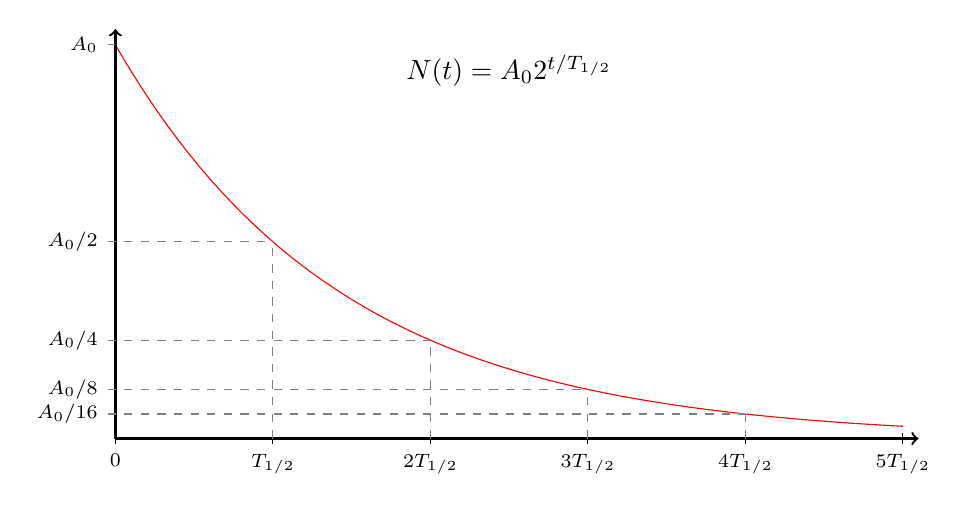
\begin{tikzpicture}
\begin{scope}[]
\clip (0,0) rectangle (10,5);
\begin{scope}[red]
\draw[] (0.0,5.0) -- (0.1,4.829681644624228);
\draw[] (0.1,4.829681644624228) -- (0.2,4.665164957684037);
\draw[] (0.2,4.665164957684037) -- (0.3,4.5062523130541505);
\draw[] (0.3,4.5062523130541505) -- (0.4,4.352752816480621);
\draw[] (0.4,4.352752816480621) -- (0.5,4.204482076268572);
\draw[] (0.5,4.204482076268572) -- (0.6,4.061261981781177);
\draw[] (0.6,4.061261981781177) -- (0.7,3.9229204894837535);
\draw[] (0.7,3.9229204894837535) -- (0.8,3.789291416275995);
\draw[] (0.8,3.789291416275995) -- (0.9,3.6602142398640636);
\draw[] (0.9,3.6602142398640636) -- (1.0,3.5355339059327378);
\draw[] (1.0,3.5355339059327378) -- (1.1,3.4151006418859886);
\draw[] (1.1,3.4151006418859886) -- (1.2,3.2987697769322355);
\draw[] (1.2,3.2987697769322355) -- (1.3,3.1864015682981552);
\draw[] (1.3,3.1864015682981552) -- (1.4,3.0778610333622907);
\draw[] (1.4,3.0778610333622907) -- (1.5,2.9730177875068025);
\draw[] (1.5,2.9730177875068025) -- (1.6,2.871745887492587);
\draw[] (1.6,2.871745887492587) -- (1.7,2.7739236801696125);
\draw[] (1.7,2.7739236801696125) -- (1.8,2.679433656340733);
\draw[] (1.8,2.679433656340733) -- (1.9,2.588162309603444);
\draw[] (1.9,2.588162309603444) -- (2.0,2.5);
\draw[] (2.0,2.5) -- (2.1,2.4148408223121134);
\draw[] (2.1,2.4148408223121134) -- (2.2,2.3325824788420184);
\draw[] (2.2,2.3325824788420184) -- (2.3,2.2531261565270757);
\draw[] (2.3,2.2531261565270757) -- (2.4,2.1763764082403103);
\draw[] (2.4,2.1763764082403103) -- (2.5,2.102241038134286);
\draw[] (2.5,2.102241038134286) -- (2.6,2.0306309908905886);
\draw[] (2.6,2.0306309908905886) -- (2.7,1.9614602447418765);
\draw[] (2.7,1.9614602447418765) -- (2.8,1.8946457081379977);
\draw[] (2.8,1.8946457081379977) -- (2.9,1.8301071199320318);
\draw[] (2.9,1.8301071199320318) -- (3.0,1.7677669529663689);
\draw[] (3.0,1.7677669529663689) -- (3.1,1.7075503209429943);
\draw[] (3.1,1.7075503209429943) -- (3.2,1.6493848884661177);
\draw[] (3.2,1.6493848884661177) -- (3.3,1.5932007841490776);
\draw[] (3.3,1.5932007841490776) -- (3.4,1.5389305166811453);
\draw[] (3.4,1.5389305166811453) -- (3.5,1.4865088937534012);
\draw[] (3.5,1.4865088937534012) -- (3.6,1.4358729437462936);
\draw[] (3.6,1.4358729437462936) -- (3.7,1.386961840084806);
\draw[] (3.7,1.386961840084806) -- (3.8,1.3397168281703664);
\draw[] (3.8,1.3397168281703664) -- (3.9,1.294081154801722);
\draw[] (3.9,1.294081154801722) -- (4.0,1.25);
\draw[] (4.0,1.25) -- (4.1,1.2074204111560571);
\draw[] (4.1,1.2074204111560571) -- (4.2,1.1662912394210092);
\draw[] (4.2,1.1662912394210092) -- (4.3,1.1265630782635379);
\draw[] (4.3,1.1265630782635379) -- (4.4,1.088188204120155);
\draw[] (4.4,1.088188204120155) -- (4.5,1.051120519067143);
\draw[] (4.5,1.051120519067143) -- (4.6,1.0153154954452943);
\draw[] (4.6,1.0153154954452943) -- (4.7,0.9807301223709383);
\draw[] (4.7,0.9807301223709383) -- (4.8,0.9473228540689989);
\draw[] (4.8,0.9473228540689989) -- (4.9,0.9150535599660157);
\draw[] (4.9,0.9150535599660157) -- (5.0,0.8838834764831844);
\draw[] (5.0,0.8838834764831844) -- (5.1,0.8537751604714973);
\draw[] (5.1,0.8537751604714973) -- (5.2,0.8246924442330589);
\draw[] (5.2,0.8246924442330589) -- (5.3,0.7966003920745388);
\draw[] (5.3,0.7966003920745388) -- (5.4,0.7694652583405726);
\draw[] (5.4,0.7694652583405726) -- (5.5,0.7432544468767006);
\draw[] (5.5,0.7432544468767006) -- (5.6,0.7179364718731469);
\draw[] (5.6,0.7179364718731469) -- (5.7,0.693480920042403);
\draw[] (5.7,0.693480920042403) -- (5.8,0.6698584140851832);
\draw[] (5.8,0.6698584140851832) -- (5.9,0.6470405774008609);
\draw[] (5.9,0.6470405774008609) -- (6.0,0.625);
\draw[] (6.0,0.625) -- (6.1,0.6037102055780286);
\draw[] (6.1,0.6037102055780286) -- (6.2,0.5831456197105046);
\draw[] (6.2,0.5831456197105046) -- (6.3,0.5632815391317689);
\draw[] (6.3,0.5632815391317689) -- (6.4,0.5440941020600775);
\draw[] (6.4,0.5440941020600775) -- (6.5,0.5255602595335715);
\draw[] (6.5,0.5255602595335715) -- (6.6,0.5076577477226472);
\draw[] (6.6,0.5076577477226472) -- (6.7,0.49036506118546913);
\draw[] (6.7,0.49036506118546913) -- (6.8,0.4736614270344994);
\draw[] (6.8,0.4736614270344994) -- (6.9,0.45752677998300784);
\draw[] (6.9,0.45752677998300784) -- (7.0,0.4419417382415922);
\draw[] (7.0,0.4419417382415922) -- (7.1,0.42688758023574863);
\draw[] (7.1,0.42688758023574863) -- (7.2,0.41234622211652944);
\draw[] (7.2,0.41234622211652944) -- (7.3,0.3983001960372694);
\draw[] (7.3,0.3983001960372694) -- (7.4,0.3847326291702863);
\draw[] (7.4,0.3847326291702863) -- (7.5,0.3716272234383503);
\draw[] (7.5,0.3716272234383503) -- (7.6,0.35896823593657345);
\draw[] (7.6,0.35896823593657345) -- (7.7,0.3467404600212015);
\draw[] (7.7,0.3467404600212015) -- (7.8,0.3349292070425916);
\draw[] (7.8,0.3349292070425916) -- (7.9,0.3235202887004304);
\draw[] (7.9,0.3235202887004304) -- (8.0,0.3125);
\draw[] (8.0,0.3125) -- (8.1,0.3018551027890143);
\draw[] (8.1,0.3018551027890143) -- (8.2,0.29157280985525236);
\draw[] (8.2,0.29157280985525236) -- (8.3,0.28164076956588435);
\draw[] (8.3,0.28164076956588435) -- (8.4,0.27204705103003873);
\draw[] (8.4,0.27204705103003873) -- (8.5,0.2627801297667858);
\draw[] (8.5,0.2627801297667858) -- (8.6,0.2538288738613236);
\draw[] (8.6,0.2538288738613236) -- (8.7,0.24518253059273465);
\draw[] (8.7,0.24518253059273465) -- (8.8,0.23683071351724963);
\draw[] (8.8,0.23683071351724963) -- (8.9,0.22876338999150392);
\draw[] (8.9,0.22876338999150392) -- (9.0,0.2209708691207961);
\draw[] (9.0,0.2209708691207961) -- (9.1,0.21344379011787432);
\draw[] (9.1,0.21344379011787432) -- (9.2,0.20617311105826477);
\draw[] (9.2,0.20617311105826477) -- (9.3,0.19915009801863465);
\draw[] (9.3,0.19915009801863465) -- (9.4,0.19236631458514314);
\draw[] (9.4,0.19236631458514314) -- (9.5,0.18581361171917515);
\draw[] (9.5,0.18581361171917515) -- (9.6,0.17948411796828673);
\draw[] (9.6,0.17948411796828673) -- (9.7,0.1733702300106008);
\draw[] (9.7,0.1733702300106008) -- (9.8,0.16746460352129575);
\draw[] (9.8,0.16746460352129575) -- (9.9,0.1617601443502152);
\draw[] (9.9,0.1617601443502152) -- (10.0,0.15625);
\end{scope}
\end{scope}
\draw (0,0cm + 2pt) -- (0, 0cm-2pt) node[below] {\scriptsize $0$};
\draw (2,0cm + 2pt) -- (2, 0cm-2pt) node[below] {\scriptsize $T_{1/2}$};
\draw (4,0cm + 2pt) -- (4, 0cm-2pt) node[below] {\scriptsize $2T_{1/2}$};
\draw (6,0cm + 2pt) -- (6, 0cm-2pt) node[below] {\scriptsize $3T_{1/2}$};
\draw (8,0cm + 2pt) -- (8, 0cm-2pt) node[below] {\scriptsize $4T_{1/2}$};
\draw (10,0cm + 2pt) -- (10, 0cm-2pt) node[below] {\scriptsize $5T_{1/2}$};
\node[below] at (5.0,5.0) {$N(t) = A_0 2^{t/T_{1/2}}$};
\draw[thick,->] (0.0,0.0) -- (0.0,5.2);
\draw[thick,->] (0.0,0.0) -- (10.2,0.0);
\draw[thin,gray,dashed] (-0.1,5.0) -- (0.0,5.0);
\node[left] at (-0.1,5.0) {\scriptsize{$A_0$}};
\draw[thin,gray,dashed] (-0.1,2.5) -- (2.0,2.5);
\draw[thin,gray,dashed] (2.0,0.0) -- (2.0,2.5);
\node[left] at (-0.1,2.5) {\scriptsize{$A_0/2$}};
\draw[thin,gray,dashed] (-0.1,1.25) -- (4.0,1.25);
\draw[thin,gray,dashed] (4.0,0.0) -- (4.0,1.25);
\node[left] at (-0.1,1.25) {\scriptsize{$A_0/4$}};
\draw[thin,gray,dashed] (-0.1,0.625) -- (6.0,0.625);
\draw[thin,gray,dashed] (6.0,0.0) -- (6.0,0.625);
\node[left] at (-0.1,0.625) {\scriptsize{$A_0/8$}};
\draw[thin,gray,dashed] (-0.1,0.3125) -- (8.0,0.3125);
\draw[thin,gray,dashed] (8.0,0.0) -- (8.0,0.3125);
\node[left] at (-0.1,0.3125) {\scriptsize{$A_0/16$}};
\end{tikzpicture}
%%% Local Variables: 
%%% mode: latex 
%%% TeX-master: "master" 
%%% End:


  \caption{Graph of radioactive decay.}
\end{figure}

\begin{figure}[H]
  \centering
  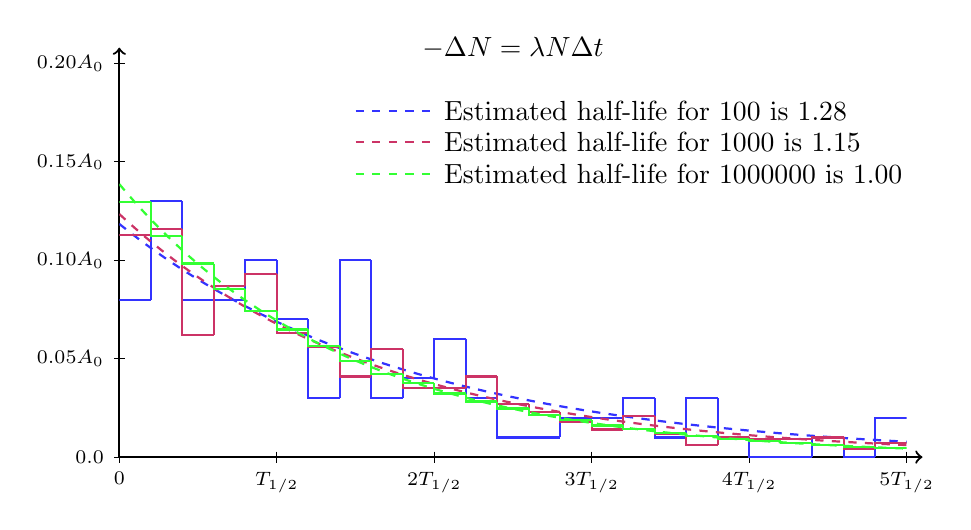
\begin{tikzpicture}
\node[] at (5.0,5.2) {$-\Delta N = \lambda N \Delta t$};
\draw[thick,->] (0.0,0.0) -- (0.0,5.2);
\draw[thick,->] (0.0,0.0) -- (10.2,0.0);
\draw (0,0cm + 2pt) -- (0, 0cm-2pt) node[below] {\scriptsize $0$};
\draw (2,0cm + 2pt) -- (2, 0cm-2pt) node[below] {\scriptsize $T_{1/2}$};
\draw (4,0cm + 2pt) -- (4, 0cm-2pt) node[below] {\scriptsize $2T_{1/2}$};
\draw (6,0cm + 2pt) -- (6, 0cm-2pt) node[below] {\scriptsize $3T_{1/2}$};
\draw (8,0cm + 2pt) -- (8, 0cm-2pt) node[below] {\scriptsize $4T_{1/2}$};
\draw (10,0cm + 2pt) -- (10, 0cm-2pt) node[below] {\scriptsize $5T_{1/2}$};
\draw (0cm+2pt,0.    ) -- (0cm-2pt,0.    ) node[left] {\scriptsize $0.0$};
\draw (0cm+2pt,1.25    ) -- (0cm-2pt,1.25    ) node[left] {\scriptsize $0.05 A_0$};
\draw (0cm+2pt,2.5    ) -- (0cm-2pt,2.5    ) node[left] {\scriptsize $0.10 A_0$};
\draw (0cm+2pt,3.750000093132256    ) -- (0cm-2pt,3.750000093132256    ) node[left] {\scriptsize $0.15 A_0$};
\draw (0cm+2pt,5.    ) -- (0cm-2pt,5.    ) node[left] {\scriptsize $0.20 A_0$};
\begin{scope}[]
\clip (0,0) rectangle (10,5);
\draw[dashed,blue!80,thick] (3.0,4.4) -- (4.0,4.4);
\node[right,] at (4.0,4.4) {Estimated half-life for 100 is  1.28};
\begin{scope}[blue!80,thick]
\draw[] (0.0,1.999999970197678) -- (0.4,1.999999970197678);
\draw (0.4,1.999999970197678) -- (0.4,3.249999951571227) -- (0.8,3.249999951571227);
\draw (0.8,3.249999951571227) -- (0.8,1.999999970197678) -- (1.2,1.999999970197678);
\draw (1.2,1.999999970197678) -- (1.2,1.999999970197678) -- (1.6,1.999999970197678);
\draw (1.6,1.999999970197678) -- (1.6,2.4999999627470975) -- (2.0,2.4999999627470975);
\draw (2.0,2.4999999627470975) -- (2.0,1.7499999739229684) -- (2.4,1.7499999739229684);
\draw (2.4,1.7499999739229684) -- (2.4,0.7499999888241292) -- (2.8,0.7499999888241292);
\draw (2.8,0.7499999888241292) -- (2.8,2.4999999627470975) -- (3.2,2.4999999627470975);
\draw (3.2,2.4999999627470975) -- (3.2,0.7499999888241292) -- (3.6000001,0.7499999888241292);
\draw (3.6000001,0.7499999888241292) -- (3.6000001,0.999999985098839) -- (4.0,0.999999985098839);
\draw (4.0,0.999999985098839) -- (4.0,1.4999999776482584) -- (4.4,1.4999999776482584);
\draw (4.4,1.4999999776482584) -- (4.4,0.7499999888241292) -- (4.8,0.7499999888241292);
\draw (4.8,0.7499999888241292) -- (4.8,0.24999999627470976) -- (5.2000003,0.24999999627470976);
\draw (5.2000003,0.24999999627470976) -- (5.2000003,0.24999999627470976) -- (5.6,0.24999999627470976);
\draw (5.6,0.24999999627470976) -- (5.6,0.4999999925494195) -- (6.0,0.4999999925494195);
\draw (6.0,0.4999999925494195) -- (6.0,0.4999999925494195) -- (6.4,0.4999999925494195);
\draw (6.4,0.4999999925494195) -- (6.4,0.7499999888241292) -- (6.8,0.7499999888241292);
\draw (6.8,0.7499999888241292) -- (6.8,0.24999999627470976) -- (7.2000003,0.24999999627470976);
\draw (7.2000003,0.24999999627470976) -- (7.2000003,0.7499999888241292) -- (7.6,0.7499999888241292);
\draw (7.6,0.7499999888241292) -- (7.6,0.24999999627470976) -- (8.0,0.24999999627470976);
\draw (8.0,0.24999999627470976) -- (8.0,0.0) -- (8.400001,0.0);
\draw (8.400001,0.0) -- (8.400001,0.0) -- (8.8,0.0);
\draw (8.8,0.0) -- (8.8,0.24999999627470976) -- (9.2,0.24999999627470976);
\draw (9.2,0.24999999627470976) -- (9.2,0.0) -- (9.6,0.0);
\draw (9.6,0.0) -- (9.6,0.4999999925494195) -- (10.0,0.4999999925494195);
\end{scope}
\begin{scope}[dashed,blue!80,thick]
\pgfpathmoveto{ \pgfqpoint {0.0cm} {2.961035269001679cm}}
\pgfpathlineto{ \pgfqpoint {0.1cm} {2.8816374412713213cm}}
\pgfpathlineto{ \pgfqpoint {0.2cm} {2.8043686037337845cm}}
\pgfpathlineto{ \pgfqpoint {0.3cm} {2.7291716691944843cm}}
\pgfpathlineto{ \pgfqpoint {0.4cm} {2.6559910812069814cm}}
\pgfpathlineto{ \pgfqpoint {0.5cm} {2.5847727730271752cm}}
\pgfpathlineto{ \pgfqpoint {0.6cm} {2.515464127668107cm}}
\pgfpathlineto{ \pgfqpoint {0.7cm} {2.448013939025868cm}}
\pgfpathlineto{ \pgfqpoint {0.8cm} {2.382372374047879cm}}
\pgfpathlineto{ \pgfqpoint {0.9cm} {2.318490935915604cm}}
\pgfpathlineto{ \pgfqpoint {1.0cm} {2.2563224282144825cm}}
\pgfpathlineto{ \pgfqpoint {1.1cm} {2.1958209200646266cm}}
\pgfpathlineto{ \pgfqpoint {1.2cm} {2.136941712186503cm}}
\pgfpathlineto{ \pgfqpoint {1.3cm} {2.0796413038765396cm}}
\pgfpathlineto{ \pgfqpoint {1.4cm} {2.0238773608682563cm}}
\pgfpathlineto{ \pgfqpoint {1.5cm} {1.9696086840551748cm}}
\pgfpathlineto{ \pgfqpoint {1.6cm} {1.9167951790523947cm}}
\pgfpathlineto{ \pgfqpoint {1.7cm} {1.8653978265743565cm}}
\pgfpathlineto{ \pgfqpoint {1.8cm} {1.8153786536069cm}}
\pgfpathlineto{ \pgfqpoint {1.9cm} {1.7667007053523203cm}}
\pgfpathlineto{ \pgfqpoint {2.0cm} {1.7193280179266968cm}}
\pgfpathlineto{ \pgfqpoint {2.1cm} {1.6732255917893186cm}}
\pgfpathlineto{ \pgfqpoint {2.2cm} {1.6283593658845843cm}}
\pgfpathlineto{ \pgfqpoint {2.3cm} {1.5846961924772622cm}}
\pgfpathlineto{ \pgfqpoint {2.4cm} {1.5422038126625208cm}}
\pgfpathlineto{ \pgfqpoint {2.5cm} {1.5008508325326482cm}}
\pgfpathlineto{ \pgfqpoint {2.6cm} {1.4606066999828298cm}}
\pgfpathlineto{ \pgfqpoint {2.7cm} {1.4214416821388707cm}}
\pgfpathlineto{ \pgfqpoint {2.8cm} {1.383326843390171cm}}
\pgfpathlineto{ \pgfqpoint {2.9cm} {1.3462340240117303cm}}
\pgfpathlineto{ \pgfqpoint {3.0cm} {1.3101358193593868cm}}
\pgfpathlineto{ \pgfqpoint {3.1cm} {1.2750055596229204cm}}
\pgfpathlineto{ \pgfqpoint {3.2cm} {1.2408172901220575cm}}
\pgfpathlineto{ \pgfqpoint {3.3cm} {1.207545752130828cm}}
\pgfpathlineto{ \pgfqpoint {3.4cm} {1.175166364216096cm}}
\pgfpathlineto{ \pgfqpoint {3.5cm} {1.1436552040764874cm}}
\pgfpathlineto{ \pgfqpoint {3.6cm} {1.1129889908682922cm}}
\pgfpathlineto{ \pgfqpoint {3.7cm} {1.0831450680052797cm}}
\pgfpathlineto{ \pgfqpoint {3.8cm} {1.0541013864197295cm}}
\pgfpathlineto{ \pgfqpoint {3.9cm} {1.0258364882722981cm}}
\pgfpathlineto{ \pgfqpoint {4.0cm} {0.9983294910986982cm}}
\pgfpathlineto{ \pgfqpoint {4.1cm} {0.9715600723814687cm}}
\pgfpathlineto{ \pgfqpoint {4.2cm} {0.9455084545354424cm}}
\pgfpathlineto{ \pgfqpoint {4.3cm} {0.9201553902958152cm}}
\pgfpathlineto{ \pgfqpoint {4.4cm} {0.8954821484980237cm}}
\pgfpathlineto{ \pgfqpoint {4.5cm} {0.8714705002389241cm}}
\pgfpathlineto{ \pgfqpoint {4.6cm} {0.848102705409048cm}}
\pgfpathlineto{ \pgfqpoint {4.7cm} {0.8253614995859841cm}}
\pgfpathlineto{ \pgfqpoint {4.8cm} {0.8032300812792068cm}}
\pgfpathlineto{ \pgfqpoint {4.9cm} {0.7816920995169194cm}}
\pgfpathlineto{ \pgfqpoint {5.0cm} {0.7607316417657523cm}}
\pgfpathlineto{ \pgfqpoint {5.1cm} {0.7403332221743797cm}}
\pgfpathlineto{ \pgfqpoint {5.2cm} {0.7204817701323781cm}}
\pgfpathlineto{ \pgfqpoint {5.3cm} {0.7011626191358686cm}}
\pgfpathlineto{ \pgfqpoint {5.4cm} {0.6823614959517176cm}}
\pgfpathlineto{ \pgfqpoint {5.5cm} {0.6640645100722925cm}}
\pgfpathlineto{ \pgfqpoint {5.6cm} {0.6462581434529782cm}}
\pgfpathlineto{ \pgfqpoint {5.7cm} {0.6289292405248749cm}}
\pgfpathlineto{ \pgfqpoint {5.8cm} {0.612064998475298cm}}
\pgfpathlineto{ \pgfqpoint {5.9cm} {0.595652957788897cm}}
\pgfpathlineto{ \pgfqpoint {6.0cm} {0.5796809930424096cm}}
\pgfpathlineto{ \pgfqpoint {6.1cm} {0.5641373039462438cm}}
\pgfpathlineto{ \pgfqpoint {6.2cm} {0.5490104066262759cm}}
\pgfpathlineto{ \pgfqpoint {6.3cm} {0.5342891251394184cm}}
\pgfpathlineto{ \pgfqpoint {6.4cm} {0.5199625832166923cm}}
\pgfpathlineto{ \pgfqpoint {6.5cm} {0.506020196227702cm}}
\pgfpathlineto{ \pgfqpoint {6.6cm} {0.4924516633605759cm}}
\pgfpathlineto{ \pgfqpoint {6.7cm} {0.47924696001159706cm}}
\pgfpathlineto{ \pgfqpoint {6.8cm} {0.46639633037889855cm}}
\pgfpathlineto{ \pgfqpoint {6.9cm} {0.45389028025475403cm}}
\pgfpathlineto{ \pgfqpoint {7.0cm} {0.4417195700111368cm}}
\pgfpathlineto{ \pgfqpoint {7.1cm} {0.4298752077733657cm}}
\pgfpathlineto{ \pgfqpoint {7.2cm} {0.4183484427767946cm}}
\pgfpathlineto{ \pgfqpoint {7.3cm} {0.40713075890163625cm}}
\pgfpathlineto{ \pgfqpoint {7.4cm} {0.3962138683811458cm}}
\pgfpathlineto{ \pgfqpoint {7.5cm} {0.38558970567851414cm}}
\pgfpathlineto{ \pgfqpoint {7.6cm} {0.37525042152794624cm}}
\pgfpathlineto{ \pgfqpoint {7.7cm} {0.3651883771355249cm}}
\pgfpathlineto{ \pgfqpoint {7.8cm} {0.3553961385355737cm}}
\pgfpathlineto{ \pgfqpoint {7.9cm} {0.3458664710983481cm}}
\pgfpathlineto{ \pgfqpoint {8.0cm} {0.3365923341850003cm}}
\pgfpathlineto{ \pgfqpoint {8.1cm} {0.3275668759458656cm}}
\pgfpathlineto{ \pgfqpoint {8.2cm} {0.3187834282582297cm}}
\pgfpathlineto{ \pgfqpoint {8.3cm} {0.3102355017998348cm}}
\pgfpathlineto{ \pgfqpoint {8.4cm} {0.30191678125448684cm}}
\pgfpathlineto{ \pgfqpoint {8.5cm} {0.29382112064621935cm}}
\pgfpathlineto{ \pgfqpoint {8.6cm} {0.285942538798569cm}}
\pgfpathlineto{ \pgfqpoint {8.7cm} {0.27827521491560686cm}}
\pgfpathlineto{ \pgfqpoint {8.8cm} {0.2708134842814604cm}}
\pgfpathlineto{ \pgfqpoint {8.9cm} {0.2635518340751504cm}}
\pgfpathlineto{ \pgfqpoint {9.0cm} {0.2564848992976483cm}}
\pgfpathlineto{ \pgfqpoint {9.1cm} {0.24960745880814725cm}}
\pgfpathlineto{ \pgfqpoint {9.2cm} {0.2429144314666177cm}}
\pgfpathlineto{ \pgfqpoint {9.3cm} {0.23640087237979632cm}}
\pgfpathlineto{ \pgfqpoint {9.4cm} {0.23006196924783684cm}}
\pgfpathlineto{ \pgfqpoint {9.5cm} {0.22389303880892142cm}}
\pgfpathlineto{ \pgfqpoint {9.6cm} {0.2178895233792081cm}}
\pgfpathlineto{ \pgfqpoint {9.7cm} {0.212046987485556cm}}
\pgfpathlineto{ \pgfqpoint {9.8cm} {0.2063611145885419cm}}
\pgfpathlineto{ \pgfqpoint {9.9cm} {0.20082770389334617cm}}
\pgfpathlineto{ \pgfqpoint {10.0cm} {0.1954426672461525cm}}
\pgfusepath{ stroke }
\end{scope}
\draw[dashed,purple!80,thick] (3.0,4.0) -- (4.0,4.0);
\node[right,] at (4.0,4.0) {Estimated half-life for 1000 is  1.15};
\begin{scope}[purple!80,thick]
\draw[] (0.0,2.8249999579042204) -- (0.4,2.8249999579042204);
\draw (0.4,2.8249999579042204) -- (0.4,2.8999999567866332) -- (0.8,2.8999999567866332);
\draw (0.8,2.8999999567866332) -- (0.8,1.5499999769032005) -- (1.2,1.5499999769032005);
\draw (1.2,1.5499999769032005) -- (1.2,2.1749999675899745) -- (1.6,2.1749999675899745);
\draw (1.6,2.1749999675899745) -- (1.6,2.3249999653548006) -- (2.0,2.3249999653548006);
\draw (2.0,2.3249999653548006) -- (2.0,1.5749999765306715) -- (2.4,1.5749999765306715);
\draw (2.4,1.5749999765306715) -- (2.4,1.3999999791383746) -- (2.8,1.3999999791383746);
\draw (2.8,1.3999999791383746) -- (2.8,1.02499998472631) -- (3.2,1.02499998472631);
\draw (3.2,1.02499998472631) -- (3.2,1.3749999795109036) -- (3.6000001,1.3749999795109036);
\draw (3.6000001,1.3749999795109036) -- (3.6000001,0.8749999869614842) -- (4.0,0.8749999869614842);
\draw (4.0,0.8749999869614842) -- (4.0,0.8749999869614842) -- (4.4,0.8749999869614842);
\draw (4.4,0.8749999869614842) -- (4.4,1.02499998472631) -- (4.8,1.02499998472631);
\draw (4.8,1.02499998472631) -- (4.8,0.6749999899417163) -- (5.2000003,0.6749999899417163);
\draw (5.2000003,0.6749999899417163) -- (5.2000003,0.5749999914318324) -- (5.6,0.5749999914318324);
\draw (5.6,0.5749999914318324) -- (5.6,0.44999999329447754) -- (6.0,0.44999999329447754);
\draw (6.0,0.44999999329447754) -- (6.0,0.34999999478459365) -- (6.4,0.34999999478459365);
\draw (6.4,0.34999999478459365) -- (6.4,0.5249999921768905) -- (6.8,0.5249999921768905);
\draw (6.8,0.5249999921768905) -- (6.8,0.29999999552965173) -- (7.2000003,0.29999999552965173);
\draw (7.2000003,0.29999999552965173) -- (7.2000003,0.14999999776482587) -- (7.6,0.14999999776482587);
\draw (7.6,0.14999999776482587) -- (7.6,0.24999999627470976) -- (8.0,0.24999999627470976);
\draw (8.0,0.24999999627470976) -- (8.0,0.22499999664723877) -- (8.400001,0.22499999664723877);
\draw (8.400001,0.22499999664723877) -- (8.400001,0.22499999664723877) -- (8.8,0.22499999664723877);
\draw (8.8,0.22499999664723877) -- (8.8,0.24999999627470976) -- (9.2,0.24999999627470976);
\draw (9.2,0.24999999627470976) -- (9.2,0.0999999985098839) -- (9.6,0.0999999985098839);
\draw (9.6,0.0999999985098839) -- (9.6,0.17499999739229682) -- (10.0,0.17499999739229682);
\end{scope}
\begin{scope}[dashed,purple!80,thick]
\pgfpathmoveto{ \pgfqpoint {0.0cm} {3.086841841736368cm}}
\pgfpathlineto{ \pgfqpoint {0.1cm} {2.9954103434620447cm}}
\pgfpathlineto{ \pgfqpoint {0.2cm} {2.9066870237421454cm}}
\pgfpathlineto{ \pgfqpoint {0.3cm} {2.820591666992095cm}}
\pgfpathlineto{ \pgfqpoint {0.4cm} {2.7370464335932585cm}}
\pgfpathlineto{ \pgfqpoint {0.5cm} {2.6559757895174174cm}}
\pgfpathlineto{ \pgfqpoint {0.6cm} {2.5773064380357407cm}}
\pgfpathlineto{ \pgfqpoint {0.7cm} {2.5009672534505296cm}}
\pgfpathlineto{ \pgfqpoint {0.8cm} {2.4268892167898066cm}}
\pgfpathlineto{ \pgfqpoint {0.9cm} {2.355005353406617cm}}
\pgfpathlineto{ \pgfqpoint {1.0cm} {2.2852506724266233cm}}
\pgfpathlineto{ \pgfqpoint {1.1cm} {2.217562107989244cm}}
\pgfpathlineto{ \pgfqpoint {1.2cm} {2.1518784622292233cm}}
\pgfpathlineto{ \pgfqpoint {1.3cm} {2.0881403499470625cm}}
\pgfpathlineto{ \pgfqpoint {1.4cm} {2.0262901449183093cm}}
\pgfpathlineto{ \pgfqpoint {1.5cm} {1.9662719277931449cm}}
\pgfpathlineto{ \pgfqpoint {1.6cm} {1.9080314355391774cm}}
\pgfpathlineto{ \pgfqpoint {1.7cm} {1.8515160123817274cm}}
\pgfpathlineto{ \pgfqpoint {1.8cm} {1.796674562197245cm}}
\pgfpathlineto{ \pgfqpoint {1.9cm} {1.7434575023168293cm}}
\pgfpathlineto{ \pgfqpoint {2.0cm} {1.691816718698071cm}}
\pgfpathlineto{ \pgfqpoint {2.1cm} {1.6417055224246973cm}}
\pgfpathlineto{ \pgfqpoint {2.2cm} {1.593078607494684cm}}
\pgfpathlineto{ \pgfqpoint {2.3cm} {1.5458920098586757cm}}
\pgfpathlineto{ \pgfqpoint {2.4cm} {1.5001030676716742cm}}
\pgfpathlineto{ \pgfqpoint {2.5cm} {1.4556703827220696cm}}
\pgfpathlineto{ \pgfqpoint {2.6cm} {1.4125537830031254cm}}
\pgfpathlineto{ \pgfqpoint {2.7cm} {1.3707142863930917cm}}
\pgfpathlineto{ \pgfqpoint {2.8cm} {1.3301140654111052cm}}
\pgfpathlineto{ \pgfqpoint {2.9cm} {1.2907164130170066cm}}
\pgfpathlineto{ \pgfqpoint {3.0cm} {1.2524857094241648cm}}
\pgfpathlineto{ \pgfqpoint {3.1cm} {1.2153873898952923cm}}
\pgfpathlineto{ \pgfqpoint {3.2cm} {1.179387913492142cm}}
\pgfpathlineto{ \pgfqpoint {3.3cm} {1.1444547327508323cm}}
\pgfpathlineto{ \pgfqpoint {3.4cm} {1.1105562642553786cm}}
\pgfpathlineto{ \pgfqpoint {3.5cm} {1.077661860082832cm}}
\pgfpathlineto{ \pgfqpoint {3.6cm} {1.0457417800942046cm}}
\pgfpathlineto{ \pgfqpoint {3.7cm} {1.014767165046131cm}}
\pgfpathlineto{ \pgfqpoint {3.8cm} {0.9847100104989565cm}}
\pgfpathlineto{ \pgfqpoint {3.9cm} {0.9555431414976606cm}}
\pgfpathlineto{ \pgfqpoint {4.0cm} {0.9272401880027255cm}}
\pgfpathlineto{ \pgfqpoint {4.1cm} {0.8997755610487362cm}}
\pgfpathlineto{ \pgfqpoint {4.2cm} {0.8731244296091581cm}}
\pgfpathlineto{ \pgfqpoint {4.3cm} {0.8472626981463717cm}}
\pgfpathlineto{ \pgfqpoint {4.4cm} {0.8221669848266726cm}}
\pgfpathlineto{ \pgfqpoint {4.5cm} {0.7978146003805356cm}}
\pgfpathlineto{ \pgfqpoint {4.6cm} {0.7741835275890351cm}}
\pgfpathlineto{ \pgfqpoint {4.7cm} {0.7512524013778684cm}}
\pgfpathlineto{ \pgfqpoint {4.8cm} {0.7290004895009958cm}}
\pgfpathlineto{ \pgfqpoint {4.9cm} {0.7074076737964186cm}}
\pgfpathlineto{ \pgfqpoint {5.0cm} {0.6864544319971635cm}}
\pgfpathlineto{ \pgfqpoint {5.1cm} {0.6661218200810166cm}}
\pgfpathlineto{ \pgfqpoint {5.2cm} {0.6463914551430555cm}}
\pgfpathlineto{ \pgfqpoint {5.3cm} {0.6272454987754936cm}}
\pgfpathlineto{ \pgfqpoint {5.4cm} {0.608666640939807cm}}
\pgfpathlineto{ \pgfqpoint {5.5cm} {0.5906380843165687cm}}
\pgfpathlineto{ \pgfqpoint {5.6cm} {0.5731435291188322cm}}
\pgfpathlineto{ \pgfqpoint {5.7cm} {0.556167158355343cm}}
\pgfpathlineto{ \pgfqpoint {5.8cm} {0.539693623530249cm}}
\pgfpathlineto{ \pgfqpoint {5.9cm} {0.52370803076638cm}}
\pgfpathlineto{ \pgfqpoint {6.0cm} {0.5081959273395551cm}}
\pgfpathlineto{ \pgfqpoint {6.1cm} {0.4931432886117389cm}}
\pgfpathlineto{ \pgfqpoint {6.2cm} {0.4785365053512349cm}}
\pgfpathlineto{ \pgfqpoint {6.3cm} {0.4643623714284517cm}}
\pgfpathlineto{ \pgfqpoint {6.4cm} {0.45060807187611746cm}}
\pgfpathlineto{ \pgfqpoint {6.5cm} {0.437261171303148cm}}
\pgfpathlineto{ \pgfqpoint {6.6cm} {0.4243096026516932cm}}
\pgfpathlineto{ \pgfqpoint {6.7cm} {0.4117416562871964cm}}
\pgfpathlineto{ \pgfqpoint {6.8cm} {0.39954596941160536cm}}
\pgfpathlineto{ \pgfqpoint {6.9cm} {0.3877115157901588cm}}
\pgfpathlineto{ \pgfqpoint {7.0cm} {0.37622759578246484cm}}
\pgfpathlineto{ \pgfqpoint {7.1cm} {0.3650838266688561cm}}
\pgfpathlineto{ \pgfqpoint {7.2cm} {0.3542701332632748cm}}
\pgfpathlineto{ \pgfqpoint {7.3cm} {0.3437767388042038cm}}
\pgfpathlineto{ \pgfqpoint {7.4cm} {0.3335941561154035cm}}
\pgfpathlineto{ \pgfqpoint {7.5cm} {0.32371317902846836cm}}
\pgfpathlineto{ \pgfqpoint {7.6cm} {0.3141248740594428cm}}
\pgfpathlineto{ \pgfqpoint {7.7cm} {0.30482057233197496cm}}
\pgfpathlineto{ \pgfqpoint {7.8cm} {0.29579186173970434cm}}
\pgfpathlineto{ \pgfqpoint {7.9cm} {0.28703057934079795cm}}
\pgfpathlineto{ \pgfqpoint {8.0cm} {0.2785288039777578cm}}
\pgfpathlineto{ \pgfqpoint {8.1cm} {0.27027884911582795cm}}
\pgfpathlineto{ \pgfqpoint {8.2cm} {0.2622732558935269cm}}
\pgfpathlineto{ \pgfqpoint {8.3cm} {0.254504786379021cm}}
\pgfpathlineto{ \pgfqpoint {8.4cm} {0.24696641702624234cm}}
\pgfpathlineto{ \pgfqpoint {8.5cm} {0.2396513323248347cm}}
\pgfpathlineto{ \pgfqpoint {8.6cm} {0.23255291863818733cm}}
\pgfpathlineto{ \pgfqpoint {8.7cm} {0.22566475822398363cm}}
\pgfpathlineto{ \pgfqpoint {8.8cm} {0.21898062343186042cm}}
\pgfpathlineto{ \pgfqpoint {8.9cm} {0.21249447107293098cm}}
\pgfpathlineto{ \pgfqpoint {9.0cm} {0.2062004369560813cm}}
\pgfpathlineto{ \pgfqpoint {9.1cm} {0.20009283058609992cm}}
\pgfpathlineto{ \pgfqpoint {9.2cm} {0.19416613001884753cm}}
\pgfpathlineto{ \pgfqpoint {9.3cm} {0.18841497686881623cm}}
\pgfpathlineto{ \pgfqpoint {9.4cm} {0.18283417146456282cm}}
\pgfpathlineto{ \pgfqpoint {9.5cm} {0.17741866814763682cm}}
\pgfpathlineto{ \pgfqpoint {9.6cm} {0.17216357071075347cm}}
\pgfpathlineto{ \pgfqpoint {9.7cm} {0.16706412797108683cm}}
\pgfpathlineto{ \pgfqpoint {9.8cm} {0.16211572947468136cm}}
\pgfpathlineto{ \pgfqpoint {9.9cm} {0.15731390132809664cm}}
\pgfpathlineto{ \pgfqpoint {10.0cm} {0.15265430215351894cm}}
\pgfusepath{ stroke }
\end{scope}
\draw[dashed,green!80,thick] (3.0,3.6) -- (4.0,3.6);
\node[right,] at (4.0,3.6) {Estimated half-life for 1000000 is  1.00};
\begin{scope}[green!80,thick]
\draw[] (0.0,3.24324995167181) -- (0.4,3.24324995167181);
\draw (0.4,3.24324995167181) -- (0.4,2.803499958224595) -- (0.8,2.803499958224595);
\draw (0.8,2.803499958224595) -- (0.8,2.4576499633781617) -- (1.2,2.4576499633781617);
\draw (1.2,2.4576499633781617) -- (1.2,2.1366749681610617) -- (1.6,2.1366749681610617);
\draw (1.6,2.1366749681610617) -- (1.6,1.8505749724242841) -- (2.0,1.8505749724242841);
\draw (2.0,1.8505749724242841) -- (2.0,1.6215999758362774) -- (2.4,1.6215999758362774);
\draw (2.4,1.6215999758362774) -- (2.4,1.412174978956953) -- (2.8,1.412174978956953);
\draw (2.8,1.412174978956953) -- (2.8,1.2185999818414452) -- (3.2,1.2185999818414452);
\draw (3.2,1.2185999818414452) -- (3.2,1.0593749842140827) -- (3.6000001,1.0593749842140827);
\draw (3.6000001,1.0593749842140827) -- (3.6000001,0.9370249860372396) -- (4.0,0.9370249860372396);
\draw (4.0,0.9370249860372396) -- (4.0,0.8068999879762532) -- (4.4,0.8068999879762532);
\draw (4.4,0.8068999879762532) -- (4.4,0.7056249894853682) -- (4.8,0.7056249894853682);
\draw (4.8,0.7056249894853682) -- (4.8,0.6178499907933177) -- (5.2000003,0.6178499907933177);
\draw (5.2000003,0.6178499907933177) -- (5.2000003,0.5375749919895084) -- (5.6,0.5375749919895084);
\draw (5.6,0.5375749919895084) -- (5.6,0.46742499303482477) -- (6.0,0.46742499303482477);
\draw (6.0,0.46742499303482477) -- (6.0,0.4023249940048904) -- (6.4,0.4023249940048904);
\draw (6.4,0.4023249940048904) -- (6.4,0.3524499947480858) -- (6.8,0.3524499947480858);
\draw (6.8,0.3524499947480858) -- (6.8,0.30812499540857974) -- (7.2000003,0.30812499540857974);
\draw (7.2000003,0.30812499540857974) -- (7.2000003,0.2634999960735441) -- (7.6,0.2634999960735441);
\draw (7.6,0.2634999960735441) -- (7.6,0.23042499656639998) -- (8.0,0.23042499656639998);
\draw (8.0,0.23042499656639998) -- (8.0,0.20917499688304964) -- (8.400001,0.20917499688304964);
\draw (8.400001,0.20917499688304964) -- (8.400001,0.17444999740049247) -- (8.8,0.17444999740049247);
\draw (8.8,0.17444999740049247) -- (8.8,0.1550249976899475) -- (9.2,0.1550249976899475);
\draw (9.2,0.1550249976899475) -- (9.2,0.1326249980237335) -- (9.6,0.1326249980237335);
\draw (9.6,0.1326249980237335) -- (9.6,0.11359999830722811) -- (10.0,0.11359999830722811);
\end{scope}
\begin{scope}[dashed,green!80,thick]
\pgfpathmoveto{ \pgfqpoint {0.0cm} {3.467170414395642cm}}
\pgfpathlineto{ \pgfqpoint {0.1cm} {3.349093928616908cm}}
\pgfpathlineto{ \pgfqpoint {0.2cm} {3.2350386055811327cm}}
\pgfpathlineto{ \pgfqpoint {0.3cm} {3.1248675022746526cm}}
\pgfpathlineto{ \pgfqpoint {0.4cm} {3.018448339357021cm}}
\pgfpathlineto{ \pgfqpoint {0.5cm} {2.915653342336934cm}}
\pgfpathlineto{ \pgfqpoint {0.6cm} {2.8163590881569953cm}}
\pgfpathlineto{ \pgfqpoint {0.7cm} {2.7204463570031265cm}}
\pgfpathlineto{ \pgfqpoint {0.8cm} {2.627799989160697cm}}
\pgfpathlineto{ \pgfqpoint {0.9cm} {2.538308746745497cm}}
\pgfpathlineto{ \pgfqpoint {1.0cm} {2.451865180143544cm}}
\pgfpathlineto{ \pgfqpoint {1.1cm} {2.3683654989993577cm}}
\pgfpathlineto{ \pgfqpoint {1.2cm} {2.287709447597804cm}}
\pgfpathlineto{ \pgfqpoint {1.3cm} {2.2098001844898802cm}}
\pgfpathlineto{ \pgfqpoint {1.4cm} {2.134544166217919cm}}
\pgfpathlineto{ \pgfqpoint {1.5cm} {2.061851035000588cm}}
\pgfpathlineto{ \pgfqpoint {1.6cm} {1.9916335102428526cm}}
\pgfpathlineto{ \pgfqpoint {1.7cm} {1.9238072837406195cm}}
\pgfpathlineto{ \pgfqpoint {1.8cm} {1.8582909184542544cm}}
\pgfpathlineto{ \pgfqpoint {1.9cm} {1.795005750729419cm}}
\pgfpathlineto{ \pgfqpoint {2.0cm} {1.733875795847841cm}}
\pgfpathlineto{ \pgfqpoint {2.1cm} {1.6748276567945994cm}}
\pgfpathlineto{ \pgfqpoint {2.2cm} {1.6177904361323991cm}}
\pgfpathlineto{ \pgfqpoint {2.3cm} {1.5626956508770122cm}}
\pgfpathlineto{ \pgfqpoint {2.4cm} {1.5094771502716904cm}}
\pgfpathlineto{ \pgfqpoint {2.5cm} {1.4580710363618128cm}}
\pgfpathlineto{ \pgfqpoint {2.6cm} {1.4084155872744135cm}}
\pgfpathlineto{ \pgfqpoint {2.7cm} {1.3604511831104658cm}}
\pgfpathlineto{ \pgfqpoint {2.8cm} {1.3141202343609497cm}}
\pgfpathlineto{ \pgfqpoint {2.9cm} {1.2693671127607487cm}}
\pgfpathlineto{ \pgfqpoint {3.0cm} {1.2261380844973617cm}}
\pgfpathlineto{ \pgfqpoint {3.1cm} {1.184381245694227cm}}
\pgfpathlineto{ \pgfqpoint {3.2cm} {1.1440464600911981cm}}
\pgfpathlineto{ \pgfqpoint {3.3cm} {1.1050852988473499cm}}
\pgfpathlineto{ \pgfqpoint {3.4cm} {1.067450982393833cm}}
\pgfpathlineto{ \pgfqpoint {3.5cm} {1.0310983242669634cm}}
\pgfpathlineto{ \pgfqpoint {3.6cm} {0.9959836768541087cm}}
\pgfpathlineto{ \pgfqpoint {3.7cm} {0.9620648789872278cm}}
\pgfpathlineto{ \pgfqpoint {3.8cm} {0.9293012053211455cm}}
\pgfpathlineto{ \pgfqpoint {3.9cm} {0.8976533174357761cm}}
\pgfpathlineto{ \pgfqpoint {4.0cm} {0.8670832166035926cm}}
\pgfpathlineto{ \pgfqpoint {4.1cm} {0.8375541981656225cm}}
\pgfpathlineto{ \pgfqpoint {4.2cm} {0.8090308074611997cm}}
\pgfpathlineto{ \pgfqpoint {4.3cm} {0.7814787972585514cm}}
\pgfpathlineto{ \pgfqpoint {4.4cm} {0.7548650866351102cm}}
\pgfpathlineto{ \pgfqpoint {4.5cm} {0.7291577212581852cm}}
\pgfpathlineto{ \pgfqpoint {4.6cm} {0.7043258350182924cm}}
\pgfpathlineto{ \pgfqpoint {4.7cm} {0.6803396129690857cm}}
\pgfpathlineto{ \pgfqpoint {4.8cm} {0.657170255529395cm}}
\pgfpathlineto{ \pgfqpoint {4.9cm} {0.634789943904375cm}}
\pgfpathlineto{ \pgfqpoint {5.0cm} {0.6131718066842659cm}}
\pgfpathlineto{ \pgfqpoint {5.1cm} {0.5922898875806458cm}}
\pgfpathlineto{ \pgfqpoint {5.2cm} {0.5721191142614477cm}}
\pgfpathlineto{ \pgfqpoint {5.3cm} {0.5526352682473172cm}}
\pgfpathlineto{ \pgfqpoint {5.4cm} {0.5338149558331651cm}}
\pgfpathlineto{ \pgfqpoint {5.5cm} {0.5156355800000055cm}}
\pgfpathlineto{ \pgfqpoint {5.6cm} {0.4980753132833515cm}}
\pgfpathlineto{ \pgfqpoint {5.7cm} {0.48111307156559274cm}}
\pgfpathlineto{ \pgfqpoint {5.8cm} {0.464728488760891cm}}
\pgfpathlineto{ \pgfqpoint {5.9cm} {0.44890189236219247cm}}
\pgfpathlineto{ \pgfqpoint {6.0cm} {0.4336142798210044cm}}
\pgfpathlineto{ \pgfqpoint {6.1cm} {0.41884729573156937cm}}
\pgfpathlineto{ \pgfqpoint {6.2cm} {0.4045832097920466cm}}
\pgfpathlineto{ \pgfqpoint {6.3cm} {0.3908048955162391cm}}
\pgfpathlineto{ \pgfqpoint {6.4cm} {0.37749580967030255cm}}
\pgfpathlineto{ \pgfqpoint {6.5cm} {0.36463997240975166cm}}
\pgfpathlineto{ \pgfqpoint {6.6cm} {0.3522219480929104cm}}
\pgfpathlineto{ \pgfqpoint {6.7cm} {0.3402268267477717cm}}
\pgfpathlineto{ \pgfqpoint {6.8cm} {0.3286402061700146cm}}
\pgfpathlineto{ \pgfqpoint {6.9cm} {0.31744817463068287cm}}
\pgfpathlineto{ \pgfqpoint {7.0cm} {0.3066372941727638cm}}
\pgfpathlineto{ \pgfqpoint {7.1cm} {0.2961945844766122cm}}
\pgfpathlineto{ \pgfqpoint {7.2cm} {0.28610750727484535cm}}
\pgfpathlineto{ \pgfqpoint {7.3cm} {0.27636395129799957cm}}
\pgfpathlineto{ \pgfqpoint {7.4cm} {0.26695221773286965cm}}
\pgfpathlineto{ \pgfqpoint {7.5cm} {0.25786100617607316cm}}
\pgfpathlineto{ \pgfqpoint {7.6cm} {0.24907940106597465cm}}
\pgfpathlineto{ \pgfqpoint {7.7cm} {0.24059685857667834cm}}
\pgfpathlineto{ \pgfqpoint {7.8cm} {0.23240319395835315cm}}
\pgfpathlineto{ \pgfqpoint {7.9cm} {0.22448856930869082cm}}
\pgfpathlineto{ \pgfqpoint {8.0cm} {0.2168434817608132cm}}
\pgfpathlineto{ \pgfqpoint {8.1cm} {0.209458752073448cm}}
\pgfpathlineto{ \pgfqpoint {8.2cm} {0.20232551360967238cm}}
\pgfpathlineto{ \pgfqpoint {8.3cm} {0.1954352016909916cm}}
\pgfpathlineto{ \pgfqpoint {8.4cm} {0.188779543313971cm}}
\pgfpathlineto{ \pgfqpoint {8.5cm} {0.18235054721707353cm}}
\pgfpathlineto{ \pgfqpoint {8.6cm} {0.17614049428577744cm}}
\pgfpathlineto{ \pgfqpoint {8.7cm} {0.17014192828445235cm}}
\pgfpathlineto{ \pgfqpoint {8.8cm} {0.1643476469038679cm}}
\pgfpathlineto{ \pgfqpoint {8.9cm} {0.1587506931135838cm}}
\pgfpathlineto{ \pgfqpoint {9.0cm} {0.15334434680883843cm}}
\pgfpathlineto{ \pgfqpoint {9.1cm} {0.14812211674190962cm}}
\pgfpathlineto{ \pgfqpoint {9.2cm} {0.14307773272825552cm}}
\pgfpathlineto{ \pgfqpoint {9.3cm} {0.13820513811808074cm}}
\pgfpathlineto{ \pgfqpoint {9.4cm} {0.1334984825242881cm}}
\pgfpathlineto{ \pgfqpoint {9.5cm} {0.12895211479808297cm}}
\pgfpathlineto{ \pgfqpoint {9.6cm} {0.1245605762437984cm}}
\pgfpathlineto{ \pgfqpoint {9.7cm} {0.12031859406479278cm}}
\pgfpathlineto{ \pgfqpoint {9.8cm} {0.11622107503255177cm}}
\pgfpathlineto{ \pgfqpoint {9.9cm} {0.11226309937139237cm}}
\pgfpathlineto{ \pgfqpoint {10.0cm} {0.10843991485142598cm}}
\pgfusepath{ stroke }
\end{scope}
\end{scope}
\end{tikzpicture}
%%% Local Variables: 
%%% mode: latex 
%%% TeX-master: "master" 
%%% End:


  \caption{Simulated number of decays per time.  Estimated half-widths from LMA.}
\end{figure}

\begin{figure}[H]
  \centering
  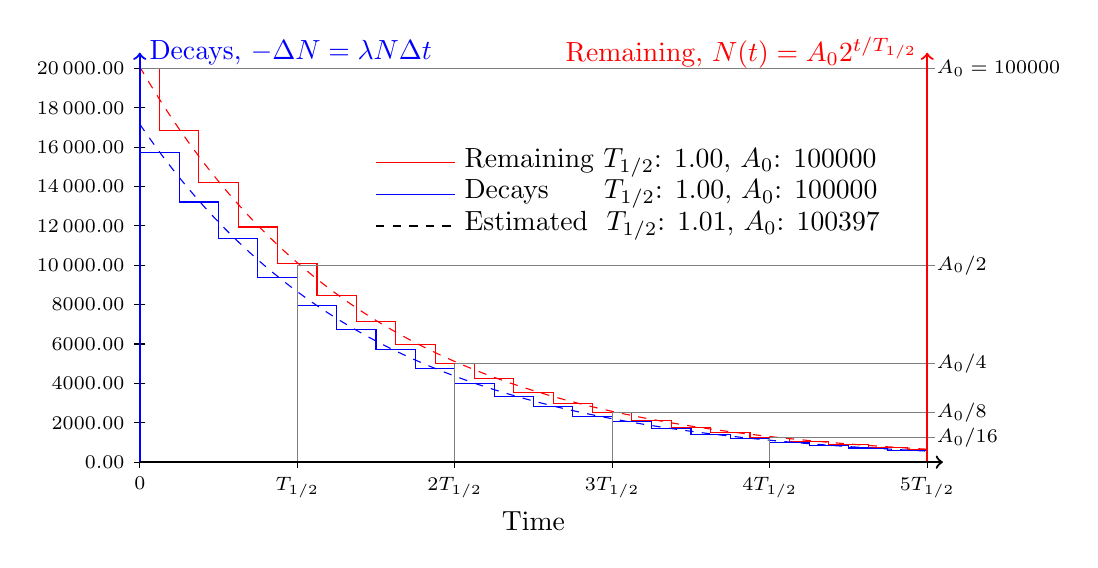
\begin{tikzpicture}
\begin{scope}[]
\clip (0,0) rectangle (10,5);
\begin{scope}[draw=blue]
\pgfpathmoveto{ \pgfqpoint {12.5cm} {0.0cm}}
\pgfpathlineto{ \pgfqpoint {12.5cm} {0.0645cm}}
\pgfpathlineto{ \pgfqpoint {12.0cm} {0.0645cm}}
\pgfpathlineto{ \pgfqpoint {12.0cm} {0.0705cm}}
\pgfpathlineto{ \pgfqpoint {11.5cm} {0.0705cm}}
\pgfpathlineto{ \pgfqpoint {11.5cm} {0.0785cm}}
\pgfpathlineto{ \pgfqpoint {11.0cm} {0.0785cm}}
\pgfpathlineto{ \pgfqpoint {11.0cm} {0.1065cm}}
\pgfpathlineto{ \pgfqpoint {10.5cm} {0.1065cm}}
\pgfpathlineto{ \pgfqpoint {10.5cm} {0.12675cm}}
\pgfpathlineto{ \pgfqpoint {10.0cm} {0.12675cm}}
\pgfpathlineto{ \pgfqpoint {10.0cm} {0.14275cm}}
\pgfpathlineto{ \pgfqpoint {9.5cm} {0.14275cm}}
\pgfpathlineto{ \pgfqpoint {9.5cm} {0.179cm}}
\pgfpathlineto{ \pgfqpoint {9.0cm} {0.179cm}}
\pgfpathlineto{ \pgfqpoint {9.0cm} {0.208cm}}
\pgfpathlineto{ \pgfqpoint {8.5cm} {0.208cm}}
\pgfpathlineto{ \pgfqpoint {8.5cm} {0.2525cm}}
\pgfpathlineto{ \pgfqpoint {8.0cm} {0.2525cm}}
\pgfpathlineto{ \pgfqpoint {8.0cm} {0.29925cm}}
\pgfpathlineto{ \pgfqpoint {7.5cm} {0.29925cm}}
\pgfpathlineto{ \pgfqpoint {7.5cm} {0.355cm}}
\pgfpathlineto{ \pgfqpoint {7.0cm} {0.355cm}}
\pgfpathlineto{ \pgfqpoint {7.0cm} {0.426cm}}
\pgfpathlineto{ \pgfqpoint {6.5cm} {0.426cm}}
\pgfpathlineto{ \pgfqpoint {6.5cm} {0.51525cm}}
\pgfpathlineto{ \pgfqpoint {6.0cm} {0.51525cm}}
\pgfpathlineto{ \pgfqpoint {6.0cm} {0.584cm}}
\pgfpathlineto{ \pgfqpoint {5.5cm} {0.584cm}}
\pgfpathlineto{ \pgfqpoint {5.5cm} {0.708cm}}
\pgfpathlineto{ \pgfqpoint {5.0cm} {0.708cm}}
\pgfpathlineto{ \pgfqpoint {5.0cm} {0.83375cm}}
\pgfpathlineto{ \pgfqpoint {4.5cm} {0.83375cm}}
\pgfpathlineto{ \pgfqpoint {4.5cm} {1.00275cm}}
\pgfpathlineto{ \pgfqpoint {4.0cm} {1.00275cm}}
\pgfpathlineto{ \pgfqpoint {4.0cm} {1.185cm}}
\pgfpathlineto{ \pgfqpoint {3.5cm} {1.185cm}}
\pgfpathlineto{ \pgfqpoint {3.5cm} {1.43475cm}}
\pgfpathlineto{ \pgfqpoint {3.0cm} {1.43475cm}}
\pgfpathlineto{ \pgfqpoint {3.0cm} {1.689cm}}
\pgfpathlineto{ \pgfqpoint {2.5cm} {1.689cm}}
\pgfpathlineto{ \pgfqpoint {2.5cm} {1.9935cm}}
\pgfpathlineto{ \pgfqpoint {2.0cm} {1.9935cm}}
\pgfpathlineto{ \pgfqpoint {2.0cm} {2.33975cm}}
\pgfpathlineto{ \pgfqpoint {1.5cm} {2.33975cm}}
\pgfpathlineto{ \pgfqpoint {1.5cm} {2.83525cm}}
\pgfpathlineto{ \pgfqpoint {1.0cm} {2.83525cm}}
\pgfpathlineto{ \pgfqpoint {1.0cm} {3.30425cm}}
\pgfpathlineto{ \pgfqpoint {0.5cm} {3.30425cm}}
\pgfpathlineto{ \pgfqpoint {0.5cm} {3.93175cm}}
\pgfpathlineto{ \pgfqpoint {0.0cm} {3.93175cm}}
\pgfpathlineto{ \pgfqpoint {0.0cm} {0.0cm}}
\pgfusepath{ stroke }
\end{scope}
\begin{scope}[draw=red]
\pgfpathmoveto{ \pgfqpoint {12.25cm} {0.0cm}}
\pgfpathlineto{ \pgfqpoint {12.25cm} {0.07965000152587891cm}}
\pgfpathlineto{ \pgfqpoint {11.75cm} {0.07965000152587891cm}}
\pgfpathlineto{ \pgfqpoint {11.75cm} {0.09375cm}}
\pgfpathlineto{ \pgfqpoint {11.25cm} {0.09375cm}}
\pgfpathlineto{ \pgfqpoint {11.25cm} {0.10945000457763672cm}}
\pgfpathlineto{ \pgfqpoint {10.75cm} {0.10945000457763672cm}}
\pgfpathlineto{ \pgfqpoint {10.75cm} {0.13075cm}}
\pgfpathlineto{ \pgfqpoint {10.25cm} {0.13075cm}}
\pgfpathlineto{ \pgfqpoint {10.25cm} {0.15610000610351563cm}}
\pgfpathlineto{ \pgfqpoint {9.75cm} {0.15610000610351563cm}}
\pgfpathlineto{ \pgfqpoint {9.75cm} {0.18465000915527344cm}}
\pgfpathlineto{ \pgfqpoint {9.25cm} {0.18465000915527344cm}}
\pgfpathlineto{ \pgfqpoint {9.25cm} {0.2204499969482422cm}}
\pgfpathlineto{ \pgfqpoint {8.75cm} {0.2204499969482422cm}}
\pgfpathlineto{ \pgfqpoint {8.75cm} {0.26205001831054686cm}}
\pgfpathlineto{ \pgfqpoint {8.25cm} {0.26205001831054686cm}}
\pgfpathlineto{ \pgfqpoint {8.25cm} {0.31255001831054685cm}}
\pgfpathlineto{ \pgfqpoint {7.75cm} {0.31255001831054685cm}}
\pgfpathlineto{ \pgfqpoint {7.75cm} {0.37239999389648437cm}}
\pgfpathlineto{ \pgfqpoint {7.25cm} {0.37239999389648437cm}}
\pgfpathlineto{ \pgfqpoint {7.25cm} {0.4433999938964844cm}}
\pgfpathlineto{ \pgfqpoint {6.75cm} {0.4433999938964844cm}}
\pgfpathlineto{ \pgfqpoint {6.75cm} {0.5286000366210938cm}}
\pgfpathlineto{ \pgfqpoint {6.25cm} {0.5286000366210938cm}}
\pgfpathlineto{ \pgfqpoint {6.25cm} {0.6316500244140625cm}}
\pgfpathlineto{ \pgfqpoint {5.75cm} {0.6316500244140625cm}}
\pgfpathlineto{ \pgfqpoint {5.75cm} {0.7484500122070312cm}}
\pgfpathlineto{ \pgfqpoint {5.25cm} {0.7484500122070312cm}}
\pgfpathlineto{ \pgfqpoint {5.25cm} {0.8900499877929687cm}}
\pgfpathlineto{ \pgfqpoint {4.75cm} {0.8900499877929687cm}}
\pgfpathlineto{ \pgfqpoint {4.75cm} {1.056800048828125cm}}
\pgfpathlineto{ \pgfqpoint {4.25cm} {1.056800048828125cm}}
\pgfpathlineto{ \pgfqpoint {4.25cm} {1.2573499755859374cm}}
\pgfpathlineto{ \pgfqpoint {3.75cm} {1.2573499755859374cm}}
\pgfpathlineto{ \pgfqpoint {3.75cm} {1.4943499755859375cm}}
\pgfpathlineto{ \pgfqpoint {3.25cm} {1.4943499755859375cm}}
\pgfpathlineto{ \pgfqpoint {3.25cm} {1.781300048828125cm}}
\pgfpathlineto{ \pgfqpoint {2.75cm} {1.781300048828125cm}}
\pgfpathlineto{ \pgfqpoint {2.75cm} {2.11910009765625cm}}
\pgfpathlineto{ \pgfqpoint {2.25cm} {2.11910009765625cm}}
\pgfpathlineto{ \pgfqpoint {2.25cm} {2.517800048828125cm}}
\pgfpathlineto{ \pgfqpoint {1.75cm} {2.517800048828125cm}}
\pgfpathlineto{ \pgfqpoint {1.75cm} {2.98575cm}}
\pgfpathlineto{ \pgfqpoint {1.25cm} {2.98575cm}}
\pgfpathlineto{ \pgfqpoint {1.25cm} {3.552800048828125cm}}
\pgfpathlineto{ \pgfqpoint {0.75cm} {3.552800048828125cm}}
\pgfpathlineto{ \pgfqpoint {0.75cm} {4.21364990234375cm}}
\pgfpathlineto{ \pgfqpoint {0.25cm} {4.21364990234375cm}}
\pgfpathlineto{ \pgfqpoint {0.25cm} {5.0cm}}
\pgfpathlineto{ \pgfqpoint {-0.25cm} {5.0cm}}
\pgfpathlineto{ \pgfqpoint {-0.25cm} {0.0cm}}
\pgfusepath{ stroke }
\end{scope}
\begin{scope}[blue,dashed]
\pgfpathmoveto{ \pgfqpoint {0.0cm} {4.291669184266502cm}}
\pgfpathlineto{ \pgfqpoint {0.1cm} {4.14738628976011cm}}
\pgfpathlineto{ \pgfqpoint {0.2cm} {4.007954084520137cm}}
\pgfpathlineto{ \pgfqpoint {0.3cm} {3.8732094917907434cm}}
\pgfpathlineto{ \pgfqpoint {0.4cm} {3.7429949173417323cm}}
\pgfpathlineto{ \pgfqpoint {0.5cm} {3.6171580651499013cm}}
\pgfpathlineto{ \pgfqpoint {0.6cm} {3.4955517592770584cm}}
\pgfpathlineto{ \pgfqpoint {0.7cm} {3.3780337717363658cm}}
\pgfpathlineto{ \pgfqpoint {0.8cm} {3.264466656145706cm}}
\pgfpathlineto{ \pgfqpoint {0.9cm} {3.1547175869734967cm}}
\pgfpathlineto{ \pgfqpoint {1.0cm} {3.0486582041889516cm}}
\pgfpathlineto{ \pgfqpoint {1.1cm} {2.946164463135092cm}}
\pgfpathlineto{ \pgfqpoint {1.2cm} {2.8471164894489163cm}}
\pgfpathlineto{ \pgfqpoint {1.3cm} {2.7513984388590553cm}}
\pgfpathlineto{ \pgfqpoint {1.4cm} {2.6588983616969335cm}}
\pgfpathlineto{ \pgfqpoint {1.5cm} {2.5695080719629626cm}}
\pgfpathlineto{ \pgfqpoint {1.6cm} {2.483123020794645cm}}
\pgfpathlineto{ \pgfqpoint {1.7cm} {2.399642174188585cm}}
\pgfpathlineto{ \pgfqpoint {1.8cm} {2.318967894833403cm}}
\pgfpathlineto{ \pgfqpoint {1.9cm} {2.241005827915344cm}}
\pgfpathlineto{ \pgfqpoint {2.0cm} {2.1656647907630173cm}}
\pgfpathlineto{ \pgfqpoint {2.1cm} {2.0928566662022066cm}}
\pgfpathlineto{ \pgfqpoint {2.2cm} {2.0224962994960154cm}}
\pgfpathlineto{ \pgfqpoint {2.3cm} {1.9545013987498094cm}}
\pgfpathlineto{ \pgfqpoint {2.4cm} {1.8887924386644783cm}}
\pgfpathlineto{ \pgfqpoint {2.5cm} {1.8252925675254414cm}}
\pgfpathlineto{ \pgfqpoint {2.6cm} {1.7639275173186217cm}}
\pgfpathlineto{ \pgfqpoint {2.7cm} {1.7046255168682534cm}}
\pgfpathlineto{ \pgfqpoint {2.8cm} {1.6473172078949372cm}}
\pgfpathlineto{ \pgfqpoint {2.9cm} {1.5919355638957637cm}}
\pgfpathlineto{ \pgfqpoint {3.0cm} {1.5384158117516333cm}}
\pgfpathlineto{ \pgfqpoint {3.1cm} {1.4866953559700764cm}}
\pgfpathlineto{ \pgfqpoint {3.2cm} {1.4367137054749826cm}}
\pgfpathlineto{ \pgfqpoint {3.3cm} {1.388412402857604cm}}
\pgfpathlineto{ \pgfqpoint {3.4cm} {1.3417349560060927cm}}
\pgfpathlineto{ \pgfqpoint {3.5cm} {1.296626772033601cm}}
\pgfpathlineto{ \pgfqpoint {3.6cm} {1.2530350934276786cm}}
\pgfpathlineto{ \pgfqpoint {3.7cm} {1.2109089363462744cm}}
\pgfpathlineto{ \pgfqpoint {3.8cm} {1.1701990309881898cm}}
\pgfpathlineto{ \pgfqpoint {3.9cm} {1.130857763968233cm}}
\pgfpathlineto{ \pgfqpoint {4.0cm} {1.0928391226296763cm}}
\pgfpathlineto{ \pgfqpoint {4.1cm} {1.0560986412288984cm}}
\pgfpathlineto{ \pgfqpoint {4.2cm} {1.0205933489292507cm}}
\pgfpathlineto{ \pgfqpoint {4.3cm} {0.9862817195433402cm}}
\pgfpathlineto{ \pgfqpoint {4.4cm} {0.9531236229649396cm}}
\pgfpathlineto{ \pgfqpoint {4.5cm} {0.9210802782337211cm}}
\pgfpathlineto{ \pgfqpoint {4.6cm} {0.8901142081779211cm}}
\pgfpathlineto{ \pgfqpoint {4.7cm} {0.8601891955818896cm}}
\pgfpathlineto{ \pgfqpoint {4.8cm} {0.8312702408272509cm}}
\pgfpathlineto{ \pgfqpoint {4.9cm} {0.8033235209581423cm}}
\pgfpathlineto{ \pgfqpoint {5.0cm} {0.7763163501226493cm}}
\pgfpathlineto{ \pgfqpoint {5.1cm} {0.7502171413441711cm}}
\pgfpathlineto{ \pgfqpoint {5.2cm} {0.724995369578007cm}}
\pgfpathlineto{ \pgfqpoint {5.3cm} {0.700621536009956cm}}
\pgfpathlineto{ \pgfqpoint {5.4cm} {0.6770671335551663cm}}
\pgfpathlineto{ \pgfqpoint {5.5cm} {0.6543046135168983cm}}
\pgfpathlineto{ \pgfqpoint {5.6cm} {0.6323073533661862cm}}
\pgfpathlineto{ \pgfqpoint {5.7cm} {0.6110496256047343cm}}
\pgfpathlineto{ \pgfqpoint {5.8cm} {0.5905065676746142cm}}
\pgfpathlineto{ \pgfqpoint {5.9cm} {0.5706541528795792cm}}
\pgfpathlineto{ \pgfqpoint {6.0cm} {0.5514691622839839cm}}
\pgfpathlineto{ \pgfqpoint {6.1cm} {0.532929157556442cm}}
\pgfpathlineto{ \pgfqpoint {6.2cm} {0.5150124547264592cm}}
\pgfpathlineto{ \pgfqpoint {6.3cm} {0.497698098823355cm}}
\pgfpathlineto{ \pgfqpoint {6.4cm} {0.48096583936779874cm}}
\pgfpathlineto{ \pgfqpoint {6.5cm} {0.46479610668730975cm}}
\pgfpathlineto{ \pgfqpoint {6.6cm} {0.4491699890280082cm}}
\pgfpathlineto{ \pgfqpoint {6.7cm} {0.43406921043585733cm}}
\pgfpathlineto{ \pgfqpoint {6.8cm} {0.4194761093815194cm}}
\pgfpathlineto{ \pgfqpoint {6.9cm} {0.4053736181038302cm}}
\pgfpathlineto{ \pgfqpoint {7.0cm} {0.39174524264773236cm}}
\pgfpathlineto{ \pgfqpoint {7.1cm} {0.37857504357331695cm}}
\pgfpathlineto{ \pgfqpoint {7.2cm} {0.365847617313416cm}}
\pgfpathlineto{ \pgfqpoint {7.3cm} {0.3535480781579374cm}}
\pgfpathlineto{ \pgfqpoint {7.4cm} {0.34166204084387597cm}}
\pgfpathlineto{ \pgfqpoint {7.5cm} {0.330175603730634cm}}
\pgfpathlineto{ \pgfqpoint {7.6cm} {0.3190753325409773cm}}
\pgfpathlineto{ \pgfqpoint {7.7cm} {0.3083482446486074cm}}
\pgfpathlineto{ \pgfqpoint {7.8cm} {0.29798179389397655cm}}
\pgfpathlineto{ \pgfqpoint {7.9cm} {0.28796385591058116cm}}
\pgfpathlineto{ \pgfqpoint {8.0cm} {0.27828271394457926cm}}
\pgfpathlineto{ \pgfqpoint {8.1cm} {0.2689270451511374cm}}
\pgfpathlineto{ \pgfqpoint {8.2cm} {0.2598859073514892cm}}
\pgfpathlineto{ \pgfqpoint {8.3cm} {0.25114872623520945cm}}
\pgfpathlineto{ \pgfqpoint {8.4cm} {0.24270528299274cm}}
\pgfpathlineto{ \pgfqpoint {8.5cm} {0.23454570236370076cm}}
\pgfpathlineto{ \pgfqpoint {8.6cm} {0.22666044108700867cm}}
\pgfpathlineto{ \pgfqpoint {8.7cm} {0.21904027673929508cm}}
\pgfpathlineto{ \pgfqpoint {8.8cm} {0.21167629694856746cm}}
\pgfpathlineto{ \pgfqpoint {8.9cm} {0.2045598889705015cm}}
\pgfpathlineto{ \pgfqpoint {9.0cm} {0.19768272961516925cm}}
\pgfpathlineto{ \pgfqpoint {9.1cm} {0.19103677551242404cm}}
\pgfpathlineto{ \pgfqpoint {9.2cm} {0.1846142537045575cm}}
\pgfpathlineto{ \pgfqpoint {9.3cm} {0.17840765255522312cm}}
\pgfpathlineto{ \pgfqpoint {9.4cm} {0.17240971296399685cm}}
\pgfpathlineto{ \pgfqpoint {9.5cm} {0.16661341987629624cm}}
\pgfpathlineto{ \pgfqpoint {9.6cm} {0.16101199407873223cm}}
\pgfpathlineto{ \pgfqpoint {9.7cm} {0.1555988842702939cm}}
\pgfpathlineto{ \pgfqpoint {9.8cm} {0.15036775940009495cm}}
\pgfpathlineto{ \pgfqpoint {9.9cm} {0.14531250126271952cm}}
\pgfpathlineto{ \pgfqpoint {10.0cm} {0.1404271973425078cm}}
\pgfusepath{ stroke }
\end{scope}
\begin{scope}[red,dashed]
\pgfpathmoveto{ \pgfqpoint {0.0cm} {5.019875113962694cm}}
\pgfpathlineto{ \pgfqpoint {0.1cm} {4.851110449118908cm}}
\pgfpathlineto{ \pgfqpoint {0.2cm} {4.688019533412946cm}}
\pgfpathlineto{ \pgfqpoint {0.3cm} {4.530411619395937cm}}
\pgfpathlineto{ \pgfqpoint {0.4cm} {4.3781023724138555cm}}
\pgfpathlineto{ \pgfqpoint {0.5cm} {4.230913655013882cm}}
\pgfpathlineto{ \pgfqpoint {0.6cm} {4.088673318598868cm}}
\pgfpathlineto{ \pgfqpoint {0.7cm} {3.9512150020862165cm}}
\pgfpathlineto{ \pgfqpoint {0.8cm} {3.8183779373357294cm}}
\pgfpathlineto{ \pgfqpoint {0.9cm} {3.690006761118823cm}}
\pgfpathlineto{ \pgfqpoint {1.0cm} {3.5659513334092017cm}}
\pgfpathlineto{ \pgfqpoint {1.1cm} {3.446066561782485cm}}
\pgfpathlineto{ \pgfqpoint {1.2cm} {3.3302122317193805cm}}
\pgfpathlineto{ \pgfqpoint {1.3cm} {3.2182528426139534cm}}
\pgfpathlineto{ \pgfqpoint {1.4cm} {3.1100574492951822cm}}
\pgfpathlineto{ \pgfqpoint {1.5cm} {3.0054995088764436cm}}
\pgfpathlineto{ \pgfqpoint {1.6cm} {2.904456732753813cm}}
\pgfpathlineto{ \pgfqpoint {1.7cm} {2.8068109435800794cm}}
\pgfpathlineto{ \pgfqpoint {1.8cm} {2.7124479370471866cm}}
\pgfpathlineto{ \pgfqpoint {1.9cm} {2.6212573483154635cm}}
\pgfpathlineto{ \pgfqpoint {2.0cm} {2.533132522933391cm}}
\pgfpathlineto{ \pgfqpoint {2.1cm} {2.4479703920969778cm}}
\pgfpathlineto{ \pgfqpoint {2.2cm} {2.3656713521028068cm}}
\pgfpathlineto{ \pgfqpoint {2.3cm} {2.286139147853802cm}}
\pgfpathlineto{ \pgfqpoint {2.4cm} {2.2092807602814393cm}}
\pgfpathlineto{ \pgfqpoint {2.5cm} {2.135006297552745cm}}
\pgfpathlineto{ \pgfqpoint {2.6cm} {2.0632288899348428cm}}
\pgfpathlineto{ \pgfqpoint {2.7cm} {1.9938645881940769cm}}
\pgfpathlineto{ \pgfqpoint {2.8cm} {1.9268322654108838cm}}
\pgfpathlineto{ \pgfqpoint {2.9cm} {1.8620535220955816cm}}
\pgfpathlineto{ \pgfqpoint {3.0cm} {1.7994525944941013cm}}
\pgfpathlineto{ \pgfqpoint {3.1cm} {1.7389562659764084cm}}
\pgfpathlineto{ \pgfqpoint {3.2cm} {1.6804937814039902cm}}
\pgfpathlineto{ \pgfqpoint {3.3cm} {1.6239967643762436cm}}
\pgfpathlineto{ \pgfqpoint {3.4cm} {1.5693991372589837cm}}
\pgfpathlineto{ \pgfqpoint {3.5cm} {1.5166370439015335cm}}
\pgfpathlineto{ \pgfqpoint {3.6cm} {1.4656487749520175cm}}
\pgfpathlineto{ \pgfqpoint {3.7cm} {1.4163746956834946cm}}
\pgfpathlineto{ \pgfqpoint {3.8cm} {1.3687571762465318cm}}
\pgfpathlineto{ \pgfqpoint {3.9cm} {1.3227405242666337cm}}
\pgfpathlineto{ \pgfqpoint {4.0cm} {1.2782709197077cm}}
\pgfpathlineto{ \pgfqpoint {4.1cm} {1.235296351925329cm}}
\pgfpathlineto{ \pgfqpoint {4.2cm} {1.193766558836341cm}}
\pgfpathlineto{ \pgfqpoint {4.3cm} {1.1536329681333846cm}}
\pgfpathlineto{ \pgfqpoint {4.4cm} {1.1148486404758622cm}}
\pgfpathlineto{ \pgfqpoint {4.5cm} {1.0773682145907377cm}}
\pgfpathlineto{ \pgfqpoint {4.6cm} {1.0411478542190187cm}}
\pgfpathlineto{ \pgfqpoint {4.7cm} {1.0061451968458563cm}}
\pgfpathlineto{ \pgfqpoint {4.8cm} {0.9723193041543079cm}}
\pgfpathlineto{ \pgfqpoint {4.9cm} {0.9396306141448049cm}}
\pgfpathlineto{ \pgfqpoint {5.0cm} {0.9080408948643329cm}}
\pgfpathlineto{ \pgfqpoint {5.1cm} {0.8775131996912039cm}}
\pgfpathlineto{ \pgfqpoint {5.2cm} {0.848011824123121cm}}
\pgfpathlineto{ \pgfqpoint {5.3cm} {0.8195022640180032cm}}
\pgfpathlineto{ \pgfqpoint {5.4cm} {0.7919511752387154cm}}
\pgfpathlineto{ \pgfqpoint {5.5cm} {0.7653263346545247cm}}
\pgfpathlineto{ \pgfqpoint {5.6cm} {0.7395966024536501cm}}
\pgfpathlineto{ \pgfqpoint {5.7cm} {0.7147318857228464cm}}
\pgfpathlineto{ \pgfqpoint {5.8cm} {0.6907031032514106cm}}
\pgfpathlineto{ \pgfqpoint {5.9cm} {0.667482151518456cm}}
\pgfpathlineto{ \pgfqpoint {6.0cm} {0.6450418718236695cm}}
\pgfpathlineto{ \pgfqpoint {6.1cm} {0.6233560185231092cm}}
\pgfpathlineto{ \pgfqpoint {6.2cm} {0.6023992283328915cm}}
\pgfpathlineto{ \pgfqpoint {6.3cm} {0.5821469906648709cm}}
\pgfpathlineto{ \pgfqpoint {6.4cm} {0.5625756189596052cm}}
\pgfpathlineto{ \pgfqpoint {6.5cm} {0.5436622229830956cm}}
\pgfpathlineto{ \pgfqpoint {6.6cm} {0.5253846820548829cm}}
\pgfpathlineto{ \pgfqpoint {6.7cm} {0.5077216191762013cm}}
\pgfpathlineto{ \pgfqpoint {6.8cm} {0.49065237602792405cm}}
\pgfpathlineto{ \pgfqpoint {6.9cm} {0.4741569888090587cm}}
\pgfpathlineto{ \pgfqpoint {7.0cm} {0.45821616488753875cm}}
\pgfpathlineto{ \pgfqpoint {7.1cm} {0.44281126023599543cm}}
\pgfpathlineto{ \pgfqpoint {7.2cm} {0.4279242576261258cm}}
\pgfpathlineto{ \pgfqpoint {7.3cm} {0.4135377455561492cm}}
\pgfpathlineto{ \pgfqpoint {7.4cm} {0.39963489788670875cm}}
\pgfpathlineto{ \pgfqpoint {7.5cm} {0.38619945416139856cm}}
\pgfpathlineto{ \pgfqpoint {7.6cm} {0.3732157005889017cm}}
\pgfpathlineto{ \pgfqpoint {7.7cm} {0.36066845166449474cm}}
\pgfpathlineto{ \pgfqpoint {7.8cm} {0.34854303240942575cm}}
\pgfpathlineto{ \pgfqpoint {7.9cm} {0.33682526120738876cm}}
\pgfpathlineto{ \pgfqpoint {8.0cm} {0.3255014332180282cm}}
\pgfpathlineto{ \pgfqpoint {8.1cm} {0.3145583043480655cm}}
\pgfpathlineto{ \pgfqpoint {8.2cm} {0.30398307576130795cm}}
\pgfpathlineto{ \pgfqpoint {8.3cm} {0.29376337890941895cm}}
\pgfpathlineto{ \pgfqpoint {8.4cm} {0.2838872610659433cm}}
\pgfpathlineto{ \pgfqpoint {8.5cm} {0.27434317134666864cm}}
\pgfpathlineto{ \pgfqpoint {8.6cm} {0.26511994719997206cm}}
\pgfpathlineto{ \pgfqpoint {8.7cm} {0.2562068013513525cm}}
\pgfpathlineto{ \pgfqpoint {8.8cm} {0.24759330918687764cm}}
\pgfpathlineto{ \pgfqpoint {8.9cm} {0.23926939656079196cm}}
\pgfpathlineto{ \pgfqpoint {9.0cm} {0.2312253280130228cm}}
\pgfpathlineto{ \pgfqpoint {9.1cm} {0.2234516953828063cm}}
\pgfpathlineto{ \pgfqpoint {9.2cm} {0.21593940680511567cm}}
\pgfpathlineto{ \pgfqpoint {9.3cm} {0.20867967607702115cm}}
\pgfpathlineto{ \pgfqpoint {9.4cm} {0.2016640123815459cm}}
\pgfpathlineto{ \pgfqpoint {9.5cm} {0.19488421035699746cm}}
\pgfpathlineto{ \pgfqpoint {9.6cm} {0.1883323405001632cm}}
\pgfpathlineto{ \pgfqpoint {9.7cm} {0.1820007398921422cm}}
\pgfpathlineto{ \pgfqpoint {9.8cm} {0.1758820032359683cm}}
\pgfpathlineto{ \pgfqpoint {9.9cm} {0.16996897419554255cm}}
\pgfpathlineto{ \pgfqpoint {10.0cm} {0.1642547370257439cm}}
\pgfusepath{ stroke }
\end{scope}
\draw[blue] (3.0,3.4) -- (4.0,3.4);
\node[right,] at (4.0,3.4) {Decays\ \ \ \ \ \ $T_{1/2}$:  1.00, $A_0$: 100000};
\draw[black,thick,dashed] (3.0,3.0) -- (4.0,3.0);
\node[right,] at (4.0,3.0) {Estimated \ $T_{1/2}$:  1.01, $A_0$: 100397};
\draw[red] (3.0,3.8) -- (4.0,3.8);
\node[right,] at (4.0,3.8) {Remaining $T_{1/2}$:  1.00, $A_0$: 100000};
\end{scope}
\draw (0.0,0.0cm + 2pt) -- (0.0, 0.0cm-2pt) node[below] {\scriptsize $0$};
\draw (2.0,0.0cm + 2pt) -- (2.0, 0.0cm-2pt) node[below] {\scriptsize $T_{1/2}$};
\draw (4.0,0.0cm + 2pt) -- (4.0, 0.0cm-2pt) node[below] {\scriptsize $2T_{1/2}$};
\draw (6.0,0.0cm + 2pt) -- (6.0, 0.0cm-2pt) node[below] {\scriptsize $3T_{1/2}$};
\draw (8.0,0.0cm + 2pt) -- (8.0, 0.0cm-2pt) node[below] {\scriptsize $4T_{1/2}$};
\draw (10.0,0.0cm + 2pt) -- (10.0, 0.0cm-2pt) node[below] {\scriptsize $5T_{1/2}$};
\draw (0.0cm + 2pt,0.0) -- (0.0cm-2pt,0.0) node[left] {\scriptsize{\num[round-mode=places,round-precision=2]{0}}};
\draw (0.0cm + 2pt,0.5) -- (0.0cm-2pt,0.5) node[left] {\scriptsize{\num[round-mode=places,round-precision=2]{2000}}};
\draw (0.0cm + 2pt,1.0) -- (0.0cm-2pt,1.0) node[left] {\scriptsize{\num[round-mode=places,round-precision=2]{4000}}};
\draw (0.0cm + 2pt,1.5) -- (0.0cm-2pt,1.5) node[left] {\scriptsize{\num[round-mode=places,round-precision=2]{6000}}};
\draw (0.0cm + 2pt,2.0) -- (0.0cm-2pt,2.0) node[left] {\scriptsize{\num[round-mode=places,round-precision=2]{8000}}};
\draw (0.0cm + 2pt,2.5) -- (0.0cm-2pt,2.5) node[left] {\scriptsize{\num[round-mode=places,round-precision=2]{10000}}};
\draw (0.0cm + 2pt,3.0) -- (0.0cm-2pt,3.0) node[left] {\scriptsize{\num[round-mode=places,round-precision=2]{12000}}};
\draw (0.0cm + 2pt,3.5) -- (0.0cm-2pt,3.5) node[left] {\scriptsize{\num[round-mode=places,round-precision=2]{14000}}};
\draw (0.0cm + 2pt,4.0) -- (0.0cm-2pt,4.0) node[left] {\scriptsize{\num[round-mode=places,round-precision=2]{16000}}};
\draw (0.0cm + 2pt,4.5) -- (0.0cm-2pt,4.5) node[left] {\scriptsize{\num[round-mode=places,round-precision=2]{18000}}};
\draw (0.0cm + 2pt,5.0) -- (0.0cm-2pt,5.0) node[left] {\scriptsize{\num[round-mode=places,round-precision=2]{20000}}};
\draw[thin,gray] (0.0,5.0) -- (10.1,5.0);
\node[right] at (10.0,5.0) {\scriptsize{$A_0 = 100000$}};
\draw[thin,gray] (2.0,2.5) -- (10.1,2.5);
\draw[thin,gray] (2.0,0.0) -- (2.0,2.5);
\node[right] at (10.0,2.5) {\scriptsize{$A_0/2$}};
\draw[thin,gray] (4.0,1.25) -- (10.1,1.25);
\draw[thin,gray] (4.0,0.0) -- (4.0,1.25);
\node[right] at (10.0,1.25) {\scriptsize{$A_0/4$}};
\draw[thin,gray] (6.0,0.625) -- (10.1,0.625);
\draw[thin,gray] (6.0,0.0) -- (6.0,0.625);
\node[right] at (10.0,0.625) {\scriptsize{$A_0/8$}};
\draw[thin,gray] (8.0,0.3125) -- (10.1,0.3125);
\draw[thin,gray] (8.0,0.0) -- (8.0,0.3125);
\node[right] at (10.0,0.3125) {\scriptsize{$A_0/16$}};
\node[right,blue] at (0.0,5.2) {Decays, $-\Delta N = \lambda N \Delta t$};
\node[left,red] at (10.0,5.2) {Remaining, $N(t) = A_0 2^{t/T_{1/2}}$};
\node[below] at (5.0,-0.5) {Time};
\draw[blue,thick,->] (0.0,0.0) -- (0.0,5.2);
\draw[red,thick,->] (10.0,0.0) -- (10.0,5.2);
\draw[thick,->] (0.0,0.0) -- (10.2,0.0);
\end{tikzpicture}
%%% Local Variables: 
%%% mode: latex 
%%% TeX-master: "master" 
%%% End:


  \caption{ Attempt to show two different axes in plot. }
\end{figure}
 
\end{document}


  
%%% Local Variables: 
%%% mode: latex
%%% TeX-master: t
%%% End: 
